% !Mode:: "TeX:UTF-8"
%%%%%%%%%%%%%%%%%%%%%%%%%%%%%%%%%%%%%%%%%%%%%%%%%%%%%%%%%%%%%%%%%%%%%%%%%%%%%%%%
%          ,
%      /\^/`\
%     | \/   |                CONGRATULATIONS!
%     | |    |             SPRING IS IN THE AIR!
%     \ \    /                                                _ _
%      '\\//'                                               _{ ' }_
%        ||                     hithesis v3                { `.!.` }
%        ||                                                ',_/Y\_,'
%        ||  ,                   dustincys                   {_,_}
%    |\  ||  |\          Email: yanshuoc@gmail.com             |
%    | | ||  | |            https://yanshuo.name             (\|  /)
%    | | || / /                                               \| //
%    \ \||/ /       https://github.com/dustincys/hithesis      |//
%      `\\//`   \\   \./    \\ /     //    \\./   \\   //   \\ |/ /
%     ^^^^^^^^^^^^^^^^^^^^^^^^^^^^^^^^^^^^^^^^^^^^^^^^^^^^^^^^^^^^^^
%%%%%%%%%%%%%%%%%%%%%%%%%%%%%%%%%%%%%%%%%%%%%%%%%%%%%%%%%%%%%%%%%%%%%%%%%%%%%%%%
\documentclass[fontset=fandol,type=bachelor,campus=harbin]{hithesisbook}
% 此处选项中不要有空格
%%%%%%%%%%%%%%%%%%%%%%%%%%%%%%%%%%%%%%%%%%%%%%%%%%%%%%%%%%%%%%%%%%%%%%%%%%%%%%%%
% 必填选项
% type=doctor|master|bachelor|postdoc
%%%%%%%%%%%%%%%%%%%%%%%%%%%%%%%%%%%%%%%%%%%%%%%%%%%%%%%%%%%%%%%%%%%%%%%%%%%%%%%%
% 选填选项(选填选项的缺省值已经尽可能满足了大多数需求,除非明确知道自己有什么
% 需求)
% campus=shenzhen|weihai|harbin
%   含义:校区选项,默认harbin
% glue=true|false
%   含义:由于我工规范中要求字体行距在一个闭区间内,这个选项为true表示tex自
%   动选择,为false表示区间内一个最接近版心要求行数的要求的默认值,缺省值为
%   false。
% tocfour=true|false
%   含义:是否添加第四级目录,只对本科文科个别要求四级目录有效,缺省值为
%   false
% fontset=windows|mac|ubuntu|fandol|adobe
%   含义:设置字体,默认情况会自动识别系统,然后设置字体。后两个是开源字体,自行
%   下载安装后设置使用。windows是中易字库,窝工默认常用字体,绝对没毛病。mac和
%   ubuntu 默认分别是华文和思源字库,理论上用什么字库都行。后两种开源字库的安装
%   方法到谷歌上百度一下什么都有了。Linux非ubuntu发行版、非x86架构机器等如何运行
%   可到github issue上讨论。
% tocblank=true|false
%   含义:目录中第一章之前,是否加一行空白。缺省值为true。
% chapterhang=true|false
%   含义:目录的章标题是否悬挂居中,规范中要求章标题少于15字,所以这个选项
%   有无没什么用,除了特殊需求。缺省值为true。
% fulltime=true|false
%   含义:是否全日制,缺省值为true。非全日制如同等学力等,要在cover中设置类
%   型,封面中不同格式
% subtitle=true|false
%   含义:论文题目是否含有副标题,缺省值为false,如果有要在cover中设置副标
%   题内容,封面中显示。
% newgeometry=one|two|no
%   含义:规范中的自相矛盾之处,版芯是否包含页眉页脚,旧方法是按照包含页眉
%   页脚来设置。该选项是多选选项,如果设置为no,则版新为旧模板的版芯设置方法,
%   如果设置该选项one或two,分别对应两种页眉页码对应版芯线的相对位置。第一种
%   是严格按照规范要求,难看。第二种微调了页眉页码位置,好一点。默认two。
% debug=true|false
%   含义:是否显示版芯框和行号,用来调试。默认否。
% openright=true|false
%   含义:博士论文是否要求章节首页必须在奇数页,此选项不在规范要求中,按个
%   人喜好自行决定。 默认否。注意,窝工的默认情况是打印版博士论文要求右翻页
%   ,电子版要求非右翻页且无空白页。如果想DIY(或身不由己DIY)在什么地方右
%   翻页,将这个选项设置为false,然后在目标位置添加`\cleardoublepage`命令即
%   可。
% library=true|false
%   含义:是否为提交到图书馆的电子版。默认否。注意:如果设置成true,那么
%   openright选项将被强制转换为false。
% capcenterlast=true|false
%   含义:图题、表题最后一行是否居中对齐(我工规范要求居中,但不要求居中对
%   齐),此选项不在规范要求中,按个人喜好自行决定。默认否。
% subcapcenterlast=true|false
%   含义:子图图题最后一行是否居中对齐(我工规范要求居中,但不要求居中对齐
%   ),此选项不在规范要求中,按个人喜好自行决定。默认否。
% absupper=true|false
%   含义:中文目录中的英文摘要在中文目录中的大小写样式歧义,在规范中要求首
%   字母大写,在work样例中是全大写。该选项控制是否全大写。默认否。
% bsmainpagenumberline=true|false
%   含义:由于本科生论文官方模板的页码和页眉格式混乱,提供这个选项自定义设
%   置是否在正文中显示页码横线,默认否。
% bsfrontpagenumberline=true|false
%   含义:由于本科生论文官方模板的页码和页眉格式混乱,提供这个选项自定义设
%   置是否在前文中显示页码横线,默认否。
% bsheadrule=true|false
%   含义:由于本科生论文官方模板的页码和页眉格式混乱,提供这个选项自定义设
%   置是否显示页眉横线,默认显示。
% splitbibitem=true|false
%   含义:参考文献每一个条目内能不能断页,应广大刀客要求添加。默认否。
% newtxmath=true|false
%   含义:数学字体是否使用新罗马。默认是。
% chapterbold=true|false
%   含义:本科生章标题在目录和正文中是否加粗
% engtoc=true|false
%   含义:非博士生需要添加英文目录的,手动添加,如果是博士,此开关无效
% zijv=word|regu
%   含义:字距设置为规范规定33个字还是word中34个字。默认regu。
%%%%%%%%%%%%%%%%%%%%%%%%%%%%%%%%%%%%%%%%%%%%%%%%%%%%%%%%%%%%%%%%%%%%%%%%%%%%%%%%
\usepackage{hithesis}

\def\dif{\mathop{}\!\mathrm{d}}
\usepackage{pythonhighlight}
\usepackage{listings}
\lstset{language=Matlab}

\usepackage{pgfplots}
\pgfplotsset{width=7cm,compat=1.8}

\graphicspath{{figures/}}

\begin{document}
\frontmatter
% !Mode:: "TeX:UTF-8"

\hitsetup{
  %******************************
  % 注意:
  %   1. 配置里面不要出现空行
  %   2. 不需要的配置信息可以删除
  %******************************
  %
  %=====
  % 秘级
  %=====
  statesecrets={公开},
  natclassifiedindex={TM301.2},
  intclassifiedindex={62-5},
  %
  %=========
  % 中文信息
  %=========
  ctitleone={基于BlazePose算法的},%本科生封面使用
  ctitletwo={机器人人体姿势识别与模仿},%本科生封面使用
  ctitlecover={基于BlazePose算法的机器人人体姿势识别与模仿},%放在封面中使用,自由断行
  ctitle={基于BlazePose算法的机器人人体姿势识别与模仿},%放在原创性声明中使用
  csubtitle={一条副标题}, %一般情况没有,可以注释掉
  cxueke={工学},
  csubject={计算机科学与技术},
  caffil={计算学部},
  cauthor={陶冶},
  csupervisor={傅忠传},
  cassosupervisor={某某某教授}, % 副指导老师
  ccosupervisor={某某某教授}, % 联合指导老师
  % 日期自动使用当前时间,若需指定按如下方式修改:
  cdate={2022年6月10日},
  newdate={2022年6月},
  cstudentid={1180300204},
  cstudenttype={学术学位论文}, %非全日制教育申请学位者
  cnumber={no9527}, %编号
  cpositionname={哈铁西站}, %博士后站名称
  cfinishdate={20XX年X月---20XX年X月}, %到站日期
  csubmitdate={20XX年X月}, %出站日期
  cstartdate={3050年9月10日}, %到站日期
  cenddate={3090年10月10日}, %出站日期
  %(同等学力人员)、(工程硕士)、(工商管理硕士)、
  %(高级管理人员工商管理硕士)、(公共管理硕士)、(中职教师)、(高校教师)等
  %
  %
  %=========
  % 英文信息
  %=========
  etitle={Research on key technologies of partial porous externally pressurized gas bearing},
  esubtitle={This is the sub title},
  exueke={Engineering},
  esubject={Computer Science and Technology},
  eaffil={\emultiline[t]{School of Mechatronics Engineering \\ Mechatronics Engineering}},
  eauthor={Yu Dongmei},
  esupervisor={Professor XXX},
  eassosupervisor={XXX},
  % 日期自动生成,若需指定按如下方式修改:
  edate={December, 2017},
  estudenttype={Master of Art},
  %
  % 关键词用“英文逗号”分割
  ckeywords={人体姿态估计, 机器人, 轻量化, 实时性, 模仿人体姿态},
  ekeywords={Human Posture Estimation, robot, lightweight, Real-time, action imitation},
}

\begin{cabstract}
人机交互的主要目的是使机器人能够学习和了解人,能领会和模仿人的语言和行为。为了是人机交互自然,必须引入类似于人与人之间的沟通方式,即依赖语音与视觉。在这种背景下,人体姿态估计在人机交互方面有着举足轻重的作用。本文就是对此提出了基于人体姿态估计的机器人姿态跟踪算法,系统地完成了足够轻量化的人体姿态估计算法,并落实到了移动端,机器人端。

本文首先系统全面地介绍了国内外对于单人姿态估计算法的发展历程以及各自的优势。并且介绍了人体姿态估计所涉及领域的主要内容,包括卷积神经网络的组成、反向传播算法、激活函数以及正则化。为后续的BlazePose算法研究打下基础。其次研究并复现了BlazePose算法,对比了复现的模型与官方模型以及一些主流模型的性能差异,在得到一个可以实用的模型后,将该算法成功部署到电脑端、手机端和机器人上。最后,得出结论:从机器人模仿的准确度和实时性而言,本项目以达到了预期的效果。

本文的主要贡献如下:

\begin{enumerate}
\item 摒弃了传统的NMS算法来进行目标检测的后处理步骤,而假设人脸必须出现在图像中并采用了一个全新的人脸检测器。

\item 将目前最主流的基于热图的姿态估计和基于回归的姿态估计相结合。使用编码器-解码器网络架构来预测所有关节的热图。同时后面跟着另一个编码器,直接回归到所有关节的坐标。使得足够轻量化,可以架构在移动端和机器人端。
\end{enumerate}
\end{cabstract}


\begin{eabstract}
The main purpose of human-computer interaction is to enable robots to learn and understand people, to comprehend and imitate human language and behavior. In order for the human-computer interaction to be natural, a communication method similar to that between humans must be introduced, that is, relying on speech and vision. In this context, human pose estimation plays a pivotal role in human-computer interaction. This paper proposes a robot posture tracking algorithm based on human body posture estimation, and systematically completes a sufficiently lightweight human body posture estimation algorithm, and implements it on the mobile side and the robot side.

This paper firstly introduces the development history of single-person pose estimation algorithms at home and abroad and their respective advantages. Then we introduced the main contents of the field of human pose estimation, including the composition of convolutional neural network, back-propagation algorithm, activation function and regularization. It lays the foundation for the follow-up BlazePose algorithm research. Secondly, the BlazePose algorithm is researched and reproduced, and the performance differences between the reproduced model and the official model and some mainstream models are compared. After obtaining a practical model, the algorithm was successfully deployed on computers, mobile phones and robots. Finally, it is concluded that this project has achieved the expected effect in terms of the accuracy and real-time performance of robot imitation.

The main contributions of this paper are as follows:

\begin{enumerate}
\item The post-processing step of the traditional NMS algorithm for object detection is abandoned, and a new face detector is adopted assuming that the face must be present in the image.

\item Combining the most mainstream heatmap-based pose estimation with regression-based pose estimation. Heatmaps for all joints are predicted using an encoder-decoder network architecture. At the same time, it is followed by another encoder, which directly returns to the coordinates of all joints. It is lightweight enough to be built on mobile and robotics.
\end{enumerate}
\end{eabstract}
 % 封面
\makecover
\begin{denotation}
\begin{table}[h]%此处最好是h
\vspace{0.5em}\centering\wuhao
\begin{tabular}{ccccc}
\toprule[1.5pt]
简称&英文全称&中文全称\\
\midrule[1pt]
CNN&Convolutional Neural Network&卷积神经网络\\
PCK&Percentage of Correct Keypoints&关键点正确估计的比例\\
HOG&Histogram of Oriented Gradient&方向梯度直方图\\
ROI&region of interest&感兴趣区域\\
NMS&non maximum suppression&非极大抑制\\
IoU&Intersection over Union&交并比\\
CPM&Convolutional Pose Machine&卷积姿态网络\\
SHN&Stacked Hourglass Networks&级联的沙漏网络\\
HRUs&Hourglass Residual Units&沙漏残差单元\\
\bottomrule[1.5pt]
\end{tabular}
\end{table}
\end{denotation}
%物理量名称表,符合规范为主,有要求添加
\tableofcontents %目录
\mainmatter
% !Mode:: "TeX:UTF-8"

\chapter{绪论}

\section{课题背景与研究意义}
单人姿态估计是计算机视觉领域的热点基础问题之一,已经研究了20多年。它之所以重要,是因为有大量的应用程序可以从这种技术中受益。例如,人体姿势估计可以在人机交互和活动识别的背景下进行更高层次的推理;它也是无标记运动捕捉(MoCap)技术的基本构建块之一。MoCap技术适用于角色动画、电影和游戏,以及病理步态的临床分析等应用。

人体姿态估计具体是指基于观察图像中的人体来恢复关节和躯干。\cite{杨川2019基于深度学习的人体姿态估计技术研究}

近年来,已有大量的成果使用到了神经网络训练姿态估计,人体姿态估计在实际生活中的应用也愈发广泛。具体如下:

\begin{enumerate}
\item 虚拟试衣

\qquad \quad 随着单人姿态估计的技术越发成熟,现在一些服饰店(如优衣库、男衣邦)推出虚拟试衣服务。以便用户省去脱衣试衣的繁琐操作,另外此项技术在疫情期间网上购物的应用场景下显然有着更光明的应用前景。图~\ref{piture:1}~便是来自ICCV2021的一篇虚拟试衣论文

\begin{figure}[h]
\centering
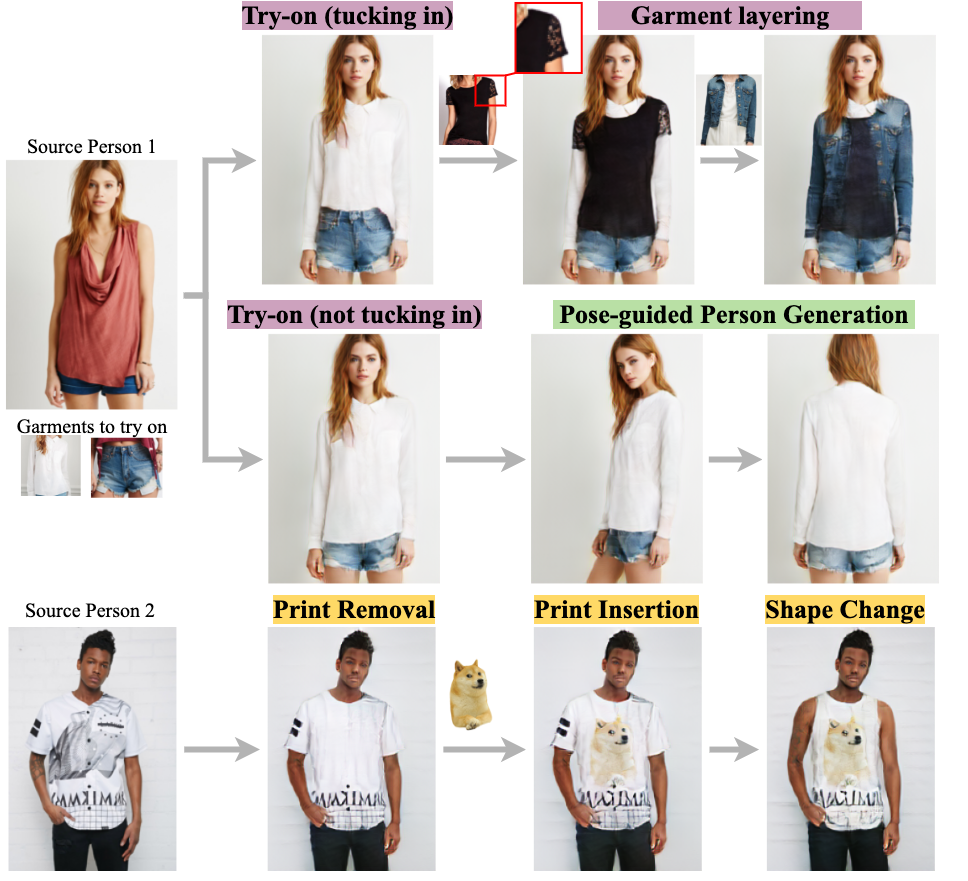
\includegraphics[width = 0.8\textwidth]{Cui_Dressing_in_Order_Recurrent_Person_Image_Generation_for_Pose_Transfer_ICCV_2021_paper_1}
\caption{不限定品类和数量的多件单品试穿,来自DiOr (Cui et al.\inlinecite{cui2021dressing})}
\label{piture:1}
\end{figure}

\item 智能安防

\qquad \quad 随着5G网络的普及,摄像头遍布公共场所,可以采集丰富的人类行为数据。现有的人体姿态估计算法已经可以分析并自动识别出监控视频中人群的活动。如存在着异常的行为,则可以即使给出异常提示或警报。\cite{戴汉彬2021基于深度学习的人体姿态估计技术研究}

\item 体育健身

\qquad \quad 疫情场景下的居家健身成为当下时代热门,如何规范、无错误动作的健身则显得尤为重要。因此,基于人体姿态估计的健身程序应运而生。该类程序运用单人姿态估计算法获取人体姿态,检测姿势是否标准,一定程度上减少了因动作不规范而引发的安全隐患。图~\ref{piture:2}~就是来自谷歌的AI健身。

\begin{figure}[h]
\centering
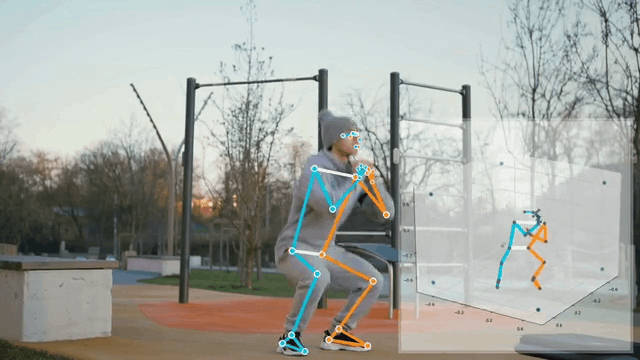
\includegraphics[width = 0.8\textwidth]{example3-13}
\caption{基于姿态估计的AI健身,来自谷歌官网}
\label{piture:2}
\end{figure}

\item VR技术

\qquad \quad 在元宇宙概念爆火的同时,也带来了一个问题,那就是VR设备动辄几万美元的费用并不是大部分人所能承担得了。作为VR体感技术的代替品,姿态估计有着得天独厚的优势,如低廉的价格、更少的硬件设备等。就目前而言,微软已有相关应用:Kinect\cite{zhang2012microsoft}。

\end{enumerate}

\section{国内外研究现状}

\subsection{基于图的人体姿态估计}

图模型、优化算法和组件外观模型是基于图的人体姿态估计方法的三个部分。该方法定义的图结构如图~\ref{piture:3}~所示。图结构模型的工作原理主要是设计一些人体部件检测器,并将各部件之间联通起来,再根据人体运动学的一些要求实现人体姿态估计。这种设计方法的主要缺点有:

\begin{enumerate}
\item 一方面,图模型结构的时间复杂度虽然较低,但是它主要提取的是HOG和SHIEFT特征,导致其无法重复使用图像的底层信息和语义信息,从而使得图像中的底层信息对于算法的制约很大。另一个,由于部件的模型较为简单,当人体运动幅度过大时,算法不能很好地识别出姿态,同一种姿态存在着多个可行解,使得图结构模型方法的应用场景比较狭隘。

\item 另一个方面,图结构模型方法基本上都是基于传统的数字图像提取特征算法,所以需要较为昂贵的专业传感设备,导致应用场景进一步受到限制。另外,这种算法通常需要多视角摄像来减少遮蔽问题,导致姿态数据的获取很是繁琐。因此,基于传统的数字图像提取特征算法来进行姿态估计无法推广,而且效率极为低效。
\end{enumerate}

\begin{figure}[h]
\centering
\includegraphics[width = 0.8\textwidth]{piture_model}
\caption{人体图结构,Felzenszwalb et al.\inlinecite{felzenszwalb2005pictorial}}
\label{piture:3}
\end{figure}

\subsection{基于深度学习的人体姿态估计}

由于技术的掣肘,在2015年之前,大部分基于深度学习的人体姿态估计都是回归精确的关键点坐标$(x,y)$,由于人体的刚性程度很低,导致这种单一方式的模型拓展性较差。因此我们主要分析15年之后的单人姿态估计算法。

MPII单人数据集是目前单人姿态估计的主流数据集之一,这可以通过计算这个数据集的PCK(Percentage of Correct Keypoints,如式(\ref{eq:1})所示)值来评估模型的优劣。目前MPII单人数据集的排名如表~\ref{performance}~所示。

\begin{equation}
\label{eq:1}
\begin{aligned}
PCK_{i}^{k}&=\frac{\sum_{p}\delta(\frac{d_{pi}}{d_{p}{def}}\leqslant T_{k})}{\sum_{p}1}\\
PCK_{mean}^{k}&=\frac{\sum_{p}\sum_{i}\delta(\frac{d_{pi}}{d_{p}{def}}\leqslant T_{k})}{\sum_{p}\sum_{i}1}
\end{aligned}
\end{equation}

\begin{table}[htbp]
\caption{Overall performance}
\label{performance}
\vspace{0.5em}\centering\wuhao
\begin{tabular}{ccccccccc}
\toprule[1.5pt]
&Head & Shoulder & Elbow & Wrist & Hip & Knee  & Ankle & Total\\
\midrule[1pt]
Pishchulin et al., ICCV'13\cite{pishchulin2013strong}& 74.3  & 49.0  & 40.8  & 34.1  & 36.5  & 34.4 & 35.2 & 44.1\\
Tompson et al., NIPS'14\cite{tompson2014joint}& 95.8  & 90.3  & 80.5  & 74.3  & 77.6  & 69.7 & 62.8 & 79.6\\
Carreira et al., CVPR'16\cite{carreira2016human}& 95.7  & 91.7  & 81.7  & 72.4  & 82.8  & 73.2 & 66.4 & 81.3\\
Tompson et al., CVPR'15\cite{tompson2015efficient}& 96.1  & 91.9  & 83.9  & 77.8  & 80.9  & 72.3 & 64.8 & 82.0\\
Hu\&Ramanan, CVPR'16\cite{hu2016bottom}& 95.0  & 91.6  & 83.0  & 76.6  & 81.9  & 74.5 & 69.5 & 82.4\\
Pishchulin et al., CVPR'16\cite{pishchulin16cvpr}& 94.1  & 90.2  & 83.4  & 77.3  & 82.6  & 75.7 & 68.6 & 82.4\\
Lifshitz et al., ECCV'16\cite{lifshitz2016human}& 97.8  & 93.3  & 85.7  & 80.4  & 85.3  & 76.6 & 70.2 & 85.0\\
Gkioxary et al., ECCV'16\cite{chain16}& 96.2  & 93.1  & 86.7  & 82.1  & 85.2  & 81.4 & 74.1 & 86.1\\
Rafi et al., BMVC'16\cite{rafi2016efficient}& 97.2  & 93.9  & 86.4  & 81.3  & 86.8  & 80.6 & 73.4 & 86.3\\
Belagiannis \& Zisserman, FG'17\cite{belagiannis2017recurrent}& 97.7  & 95.0  & 88.2  & 83.0  & 87.9  & 82.6 & 78.4 & 88.1\\
Insafutdinov et al., ECCV'16\cite{insafutdinov16ariv}& 96.8  & 95.2  & 89.3  & 84.4  & 88.4  & 83.4 & 78.0 & 88.5\\
Wei et al., CVPR'16\cite{wei2016convolutional}& 97.8  & 95.0  & 88.7  & 84.0  & 88.4  & 82.8 & 79.4 & 88.5\\
Bulat \& Tzimiropoulos, ECCV'16\cite{bulat2016human}& 97.9  & 95.1  & 89.9  & 85.3  & 89.4  & 85.7 & 81.7 & 89.7\\
Newell et al., ECCV'16\cite{newell2016stacked}& 98.2  & 96.3  & 91.2  & 87.1  & 90.1  & 87.4 & 83.6 & 90.9\\
Tang et al., ECCV'18\cite{tang2018quantized}& 97.4  & 96.4  & 92.1  & 87.7  & 90.2  & 87.7 & 84.3 & 91.2\\
Ning et al., TMM'17\cite{ning2017knowledge}& 98.1  & 96.3  & 92.2  & 87.8  & 90.6  & 87.6 & 82.7 & 91.2\\
Luvizon et al., arXiv'17\cite{DBLP:journals/corr/abs-1710-02322}& 98.1  & 96.6  & 92.0  & 87.5  & 90.6  & 88.0 & 82.7 & 91.2\\
Chu et al., CVPR'17\cite{chu2017multi}& 98.5  & 96.3  & 91.9  & 88.1  & 90.6  & 88.0 & 85.0 & 91.5\\
Chou et al., arXiv'17\cite{DBLP:journals/corr/ChouCC17}& 98.2  & 96.8  & 92.2  & 88.0  & 91.3  & 89.1 & 84.9 & 91.8\\
Chen et al., ICCV'17\cite{chen2017adversarial}& 98.1  & 96.5  & 92.5  & 88.5  & 90.2  & 89.6 & 86.0 & 91.9\\
Yang et al., ICCV'17\cite{yang2017learning}& 98.5  & 96.7  & 92.5  & 88.7  & 91.1  & 88.6 & 86.0 & 92.0\\
Ke et al., ECCV'18\cite{Ke_2018_ECCV}& 98.5  & 96.8  & 92.7  & 88.4  & 90.6  & 89.4 & 86.3 & 92.1\\
Tang et al., ECCV'18\cite{Tang_2018_ECCV}& 98.4  & 96.9  & 92.6  & 88.7  & 91.8  & 89.4 & 86.2 & 92.3\\
Zhang et al., arXiv'19\cite{zhang2019human}& 98.6  & 97.0  & 92.8  & 88.8  & 91.7  & 89.8  & 86.6  & 92.5\\
Su et al., arXiv'19\cite{su2019cascade}& 98.7  & 97.5  & 94.3  & 90.7  & 93.4  & 92.2  & 88.4  & 93.9\\
Bulat et al., FG'2020\cite{bulat2020toward}& 98.8  & 97.5  & 94.4  & 91.2  & 93.2  & 92.2  & 89.3  & 94.1\\
\bottomrule[1.5pt]
\end{tabular}
\end{table}



大体上表~\ref{performance}~中的算法可以分成两类:
\begin{itemize}
\item 基于热图的方法
\item 基于回归的方法
\end{itemize}

热力图方法能以较小的算力开销拓展到多人姿态识别,但会使得模型更复杂。

而基于回归的算法虽然计算简单,但也有一定的缺陷。最致命的是,基于回归的方法通过预测平均值并不能解决多义性问题。

Pfister et al.\inlinecite{pfister2015flowing}首次提出了回归heatmap,同时使用了网络层次较深的卷积神经网络进行姿态估计,将单人姿态估计的鲁棒性进一步提高,并且可以可视化观察训练过程,以便即使调整网络结构,避免不必要的能耗。Pfister最具创意的地方在于提出了空间融合模型,即将CNN的第三层和第七层分别提取出来再进行一次卷积操作;同时还使用了光流信息,预测出相邻帧的热力图,减少了模型的复杂度。最后经过一个池化层将对齐的热力图合成一个置信图。

Wei et al.\inlinecite{wei2016convolutional}提出了CPM(Convolutional Pose Machine)算法,使用卷积神经网络进行人体姿态估计,它的创新点在于卷积结构是高度顺序化的,表现在网络分成了多个阶段,每个阶段都会监督训练,可以更好地融合空间、纹理信息。另外还使用了多尺度处理输入,提升了模型的准确度。

Newell et al.\inlinecite{newell2016stacked}提出了SHN(Stacked Hourglass Networks)算法,使用了沙漏结构,在参数量减少的同时,又能兼顾到基于回归的姿态估计方法的准确度。SHN算法重复使用自底向上/自顶向下地网络结构,看起来像一个沙漏,故此得名。另外,同时引入了中间监督学习,从而显著提高了模型的准确率。

王晓刚组于2017年提出structured pose\cite{chu2016structured},网络结构同样是基于CNN,它在卷积层使用了几何变换核,并引入双向树概念,使得关键点的通道可以互相接受信息,从而达到信息传递的作用。与王晓刚组不同的是,Chen et al.\inlinecite{chen2017adversarial}网络结构基于GAN,性能提升效果并不显著,更多的是对于沙漏网络之后的参数微调。

Ke et al.\inlinecite{Ke_2018_ECCV}将多内容信息注意力机制迁移到卷积神经网络,得到了单人姿态估计的端到端框架,并且改进了hourglass网络架构,设计出新颖的HRUs(Hourglass Residual Units),以增加网络接受野。同时还是用了多尺度监督来训练模型,多尺度回归来优化人体结构。最后又使用了keypoint masking作为数据扩增的方式。

Tang et al.\inlinecite{Tang_2018_ECCV}设计了基于DNN的网络结构,新颖的地方在于,这个网络结构是分层组成的,并且在推理阶段使用了自下而上/自上而下。

百度研究院和香港科技大学联合于2019年出品了一篇单人pose检测文章\cite{zhang2019human}。这篇文章的贡献主要是提出了两个简单高效的模块,第一个是Cascade Prediction Fusion(CPF)网络,可以用来预测人体姿态关键点;另外一个是Pose Graph Neural Network(PGNN),用于修正预测的关键点。

2019年南京开发团队(平安科技所著)的一篇论文\cite{su2019cascade}里的算法在mpll数据集中的准确率达到93.9\%,与之前其他的单人姿态估计算法相比,准确度有着明显的提升。这主要归功于作者提出了三点创新。第一,最后将多个热图的平均值作为最后输出,提高了模型的鲁棒性;第二,联合了resnet101模型和resnet50模型,使得效果达到最佳;第三,在数据集方面,引入AI Challenger数据集起到正则化的作用。

Bulat et al.\inlinecite{bulat2020toward}设计小的block和feature map的融合方式,提人体姿态估计高计算效率和精度。该模型在MPII和LSP数据集上实现了SOTA。此外,在模型的复杂度降低三倍的情况下,运行速度提升了两倍,并且性能没有下降。在mpll数据集结果达到94.1\%。

\section{论文主要研究内容及创新点}
本文以谷歌闭源工业级模型BlazePose为切入点,优化其网络结构,完成代码复现工作,得到一个较好的模型,并利用该模型完成了对于图片、视频和摄像头实时的检测工作,并且成功将其移植到手机端、unity虚拟机器人和真实机器人上。

与之前的姿态估计算法相比,BlazePose的主要创新性工作如下:

\begin{itemize}
\item 提出了detector-tracker设计的推理通道

\qquad \quad 流程包括一个轻量级的人体姿态估计检测器和一个姿态跟踪网络。跟踪网络预测关键点坐标。当画面中第一次出现人体时,我们启动人体检测器,定位出ROI(region of interest),随后跟踪器在ROI上预测33个关键点;当画面中不是第一次出现人体(即当前帧的前一帧出现了人体),我们不会启用检测器,而是直接从上一帧的关键点推导出ROI。这样会大大提升模型的轻量化。


\item 提出了基于人脸的人检测器,

\qquad \quad 目前主流的人体姿态估计算法在检测人体的后处理步骤中,都是使用的NMS(non maximum suppression)算法,不过NMS对于非刚性物体并不是很友好,尤其是类似与人体这类关节复杂度高的姿势场景。这是因为有大量的,模糊的候选框都满足非最大值抑制的交并比阈值。

\qquad \quad 注意到人脸比较刚性,特征的对比度相对较高,所以我们假设人脸是始终可见的。对于如何检测人脸,我们使用了一个由Bazarevsky et al.提出的BlazeFace\cite{bazarevsky2019blazeface}模型。

\item 将基于热图方法和基于回归方法相结合

\qquad \quad 结合两者的优点,使用编码器-解码器网络架构来预测所有关节的热图。同时后面跟着另一个编码器,直接回归到所有关节的坐标。值得注意的是,热图分支可以在推理过程中被丢弃,使得模型足够轻量级,可以在移动端上运行。
\end{itemize}

\section{论文章节安排}

本文共五章。绪论主要介绍了论文工作的研究背景和应用场景,对国内外的人体姿态估计算法做出了一个较为详细的概况,最后概述了本项目的工作内容和创新点。

第二章介绍了有关深度学习的基础知识和基本概念以及本文用到的损失函数,激活函数,优化方法等。

第三章主要介绍了Blaze算法的推理通道,神经网络结构,人体检测器,人体拓扑结构,复现过程等。

第四章是成果展示,主要包括了五个方面:

\begin{itemize}
\item 与官方模型及其他模型的性能对比;
\item 适用于pc端的图片检测、视频检测和摄像头检测;
\item 适用于手机移动端的摄像头实时检测;
\item 在unity端虚拟机器人的检测;
\item 使用arduino开发板驱动sg90舵机完成最终的机器人姿态模仿。
\end{itemize}

% Local Variables:
% TeX-master: "../thesis"
% TeX-engine: xetex
% End:
% !Mode:: "TeX:UTF-8"

\chapter{姿态估计相关理论基础}

\section{引言}

人体姿态估计是人机交互的基础,学者们做了很多工作。从基于传感器的模型,到基于图模型的研究,再到如今基于深度学习方法的流行,其热度始终不减。但依旧无法满足应用场景。从绪论我们可以看出,当今人体姿态估计算法的方向是轻量化,快速化,准确化。

本章节主要介绍一些比较基础但十分重要的深度学习概念,为下面BlazePose算法的诞生做铺垫。首先我们会介绍卷积神经网络的各个组成部件,其次会深入了解反向传播算法,然后介绍常见的激活函数,最后为抑制过拟合现象介绍一些正则化方法。

\section{卷积神经网络的组成}

一个基本的卷积神经网络是由多个卷积层与池化层组成的卷积块以及全连接层相互连接而成。如图~\ref{piture:4}~所示。由$M(2\leqslant M\leqslant 5)$个连续的卷积层和$b(b\text{取}0\text{或}1)$个池化层组成一个卷积模块。再由$N$个连续的卷积模块和$K(0\leqslant K\leqslant 2)$个全连接层堆叠而成。

\begin{figure}[h]
\centering
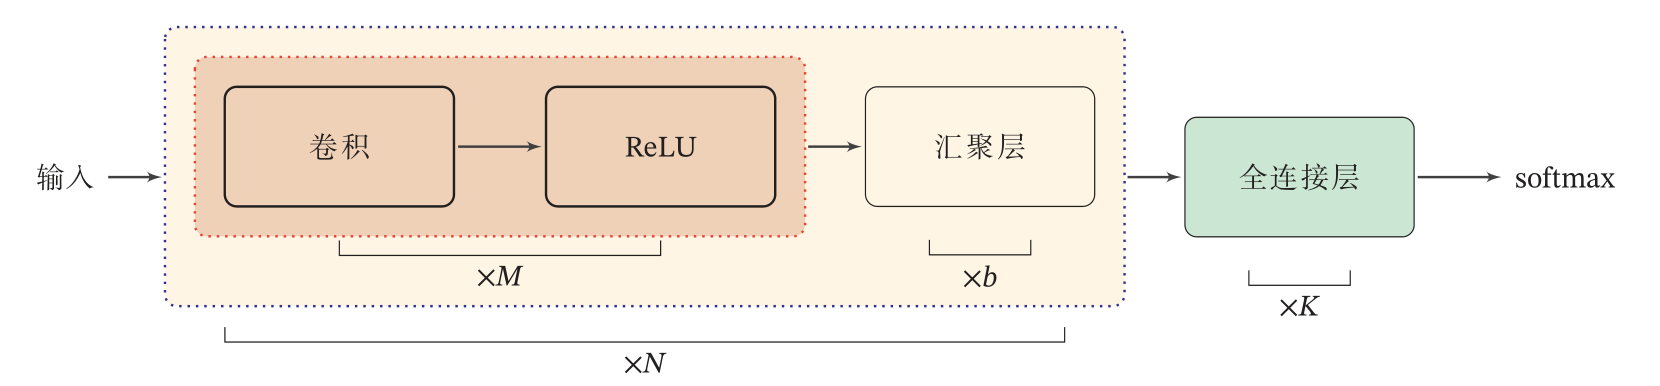
\includegraphics[width = 1\textwidth]{net}
\caption{常用卷积网络整体结构}
\label{piture:4}
\end{figure}

\subsection{卷积层}
卷积层的作用是提取特征,浅层网络可以提取到边缘,颜色等浅层信息;深层网络可以提取到形状,图案等深层的语义信息。其中,使用不同的滤波器即卷积核,提取到的信息也不尽相同。不失一般性,我们假设卷积神经网络处理的是二维图像,那么我们将通常使用三维的、大小是$M\times N\times D$神经层,其中$M,N,D$分别为高度,宽度,深度。

由此可以假设卷积层的结构如下:

\begin{enumerate}
\item 由三维张量$x\in \mathbb{R}^{M\times N\times D}$组成的输入特征映射组,其中$1\leqslant d\leqslant D$;

\item 由三维张量$y\in \mathbb{R}^{M'\times N'\times P}$组成的输出特征映射组,其中$1\leqslant p\leqslant P$;

\item 由四维张量$w\in \mathbb{R}^{U\times V\times P\times D}$组成的卷积核,其中$1\leqslant p\leqslant P,1\leqslant d\leqslant D$。
\end{enumerate}

卷积层的三维结构表示如图~\ref{piture:5}~所示。

\begin{figure}[h]
\centering
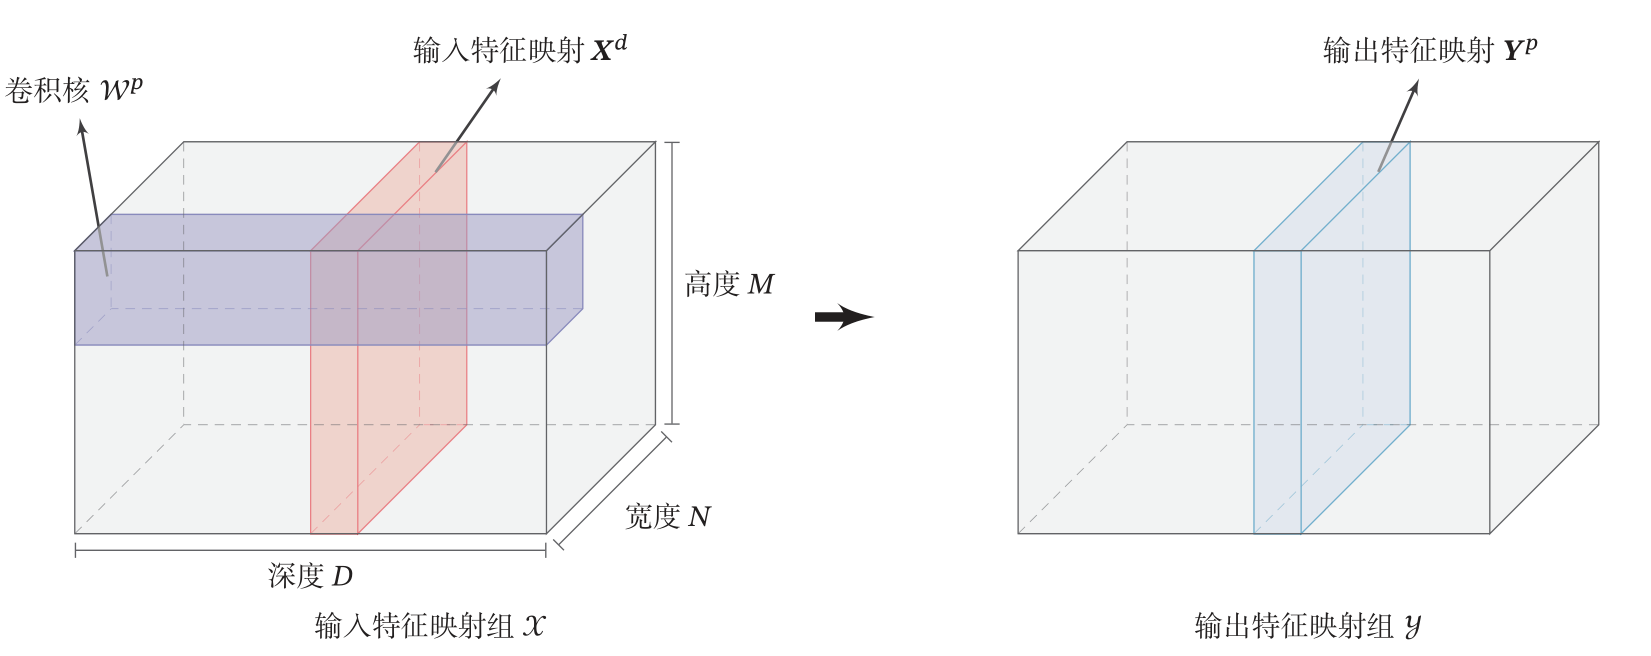
\includegraphics[width = 1\textwidth]{3-d}
\caption{卷积层的三维结构表示}
\label{piture:5}
\end{figure}

将卷积核$W^{p,1},W^{p,2},\cdots,W^{p,D}$和输入特征映射$X^1,X^2,\cdots,X^D$一一对应分别进行卷积操作,并与偏置量$b$求和。可以得到卷积层输出$Z^p$,最后再经过激活函数的激活,即可得到输出特征映射$Y^{p}$。

\begin{equation}
\label{eq:2}
\begin{aligned}
Z^p&=W^p\otimes X+b^p=\sum_{d=1}^{D}W^{p,d}\otimes X^d+b^p\\
Y^p&=f(Z^p)
\end{aligned}
\end{equation}

值得注意的是,对于激活函数$f(\cdot)$,我们一般使用ReLU函数。

计算过程的流程图如图~\ref{piture:6}~所示。

\begin{figure}[h]
\centering
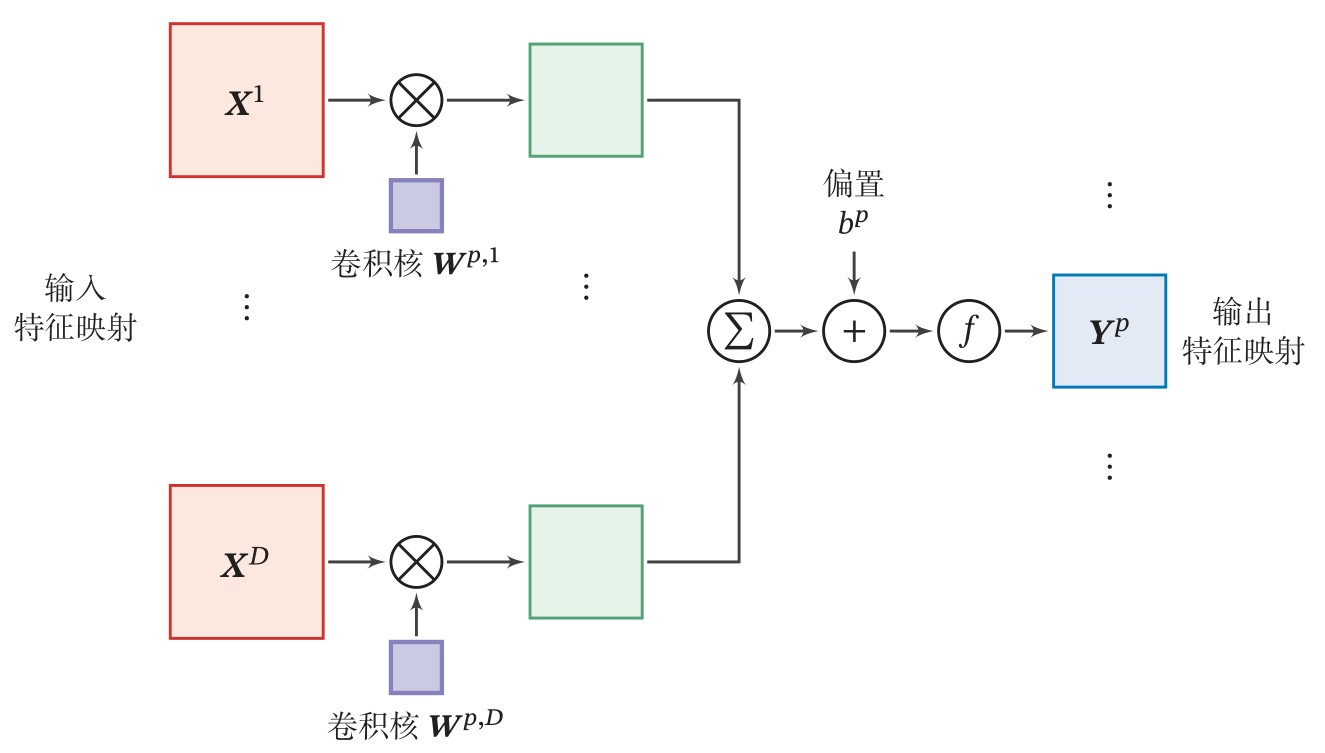
\includegraphics[width = 0.6\textwidth]{count}
\caption{卷积层中的计算流程图}
\label{piture:6}
\end{figure}

\subsection{池化层}

池化层通俗地说,池化就是将矩阵的各个子矩阵压缩。例如,如果我们想对一个$4\times 4$的矩阵进行$2\times 2$的池化,那么就会将$4\times 4$的矩阵拆分成$4$个$2\times 2$的子矩阵。并将每个子矩阵经过池化变成一个标量。一般而言,池化标准可以是最大池化,也可以是平均池化。对于前者,在每个子矩阵的元素中取出一个最大的作为结果;对于后者,则是将子矩阵的各个元素的平均值作为结果。从而达到降维的效果。

接下来,我们举一个采用$2\times 2$最大池化,步幅为$2$的例子。如图~\ref{piture:6}~所示。

首先,我们以一个$4\times 4$的输入矩阵为例,将其拆分成$4$个$2\times 2$的子矩阵。对左上角的红色子矩阵使用最大池化,得到池化结果是该区域的最大值$6$。以此类推,右上角的绿色矩阵结果为$8$,左下角的黄色区域池化结果为$3$,右下角的蓝色区域结果为$4$。最终我们得到了一个$2\times 2$的矩阵,即池化的最终结果。可以看出,池化可以在保留一定的原信息的同时有效地降低矩阵维数,简化后续计算。


\begin{figure}[h]
\centering
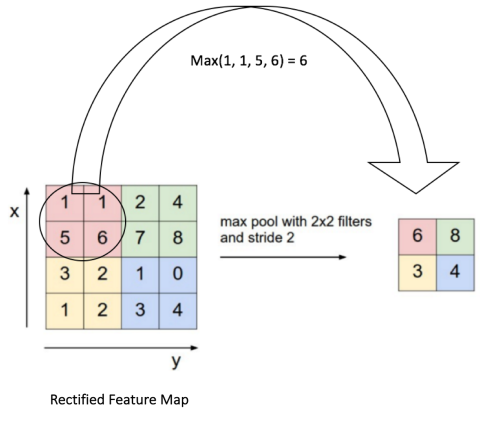
\includegraphics[width = 0.7\textwidth]{pool}
\caption{卷积层中从输入特征映射组$X$到输出特征映射$Y^p$的计算示例}
\label{piture:7}
\end{figure}

\section{卷积神经网络(CNN)反向传播算法}

\subsection{DNN的反向传播算法}

要计算DNN的反向传播,我们首先得出输出层的$\delta^L$

\begin{equation}
\label{eq:3}
\delta^L = \frac{\partial J(W,b)}{\partial z^L} = \frac{\partial J(W,b)}{\partial a^L}\odot \sigma^{'}(z^L)
\end{equation}

此外,使用第一数学归纳法,可以由$\delta^{l+1}$的值算出$\delta^l$如下:

\begin{equation}
\label{eq:4}
\delta^{l} = \delta^{l+1}\frac{\partial z^{l+1}}{\partial z^{l}} = (W^{l+1})^T\delta^{l+1}\odot \sigma^{'}(z^l)
\end{equation}

最后,我们可以得到出$W,b$的梯度:

\begin{equation}
\label{eq:5}
\begin{aligned}
\frac{\partial J(W,b)}{\partial W^l} &= \frac{\partial J(W,b,x,y)}{\partial z^l} \frac{\partial z^l}{\partial W^l} = \delta^{l}(a^{l-1})^T\\
\frac{\partial J(W,b,x,y)}{\partial b^l} &= \frac{\partial J(W,b)}{\partial z^l} \frac{\partial z^l}{\partial b^l} = \delta^{l}
\end{aligned}
\end{equation}

简单介绍完DNN的反向传播算法的推到思路后,我们将公式套用到CNN中,但需要注意的是,CNN与DNN还是有些许不同,这导致了我们需要解决几个问题,才能正确地套用。

\subsection{CNN的反向传播算法思想}

鉴于DNN与CNN的区别,我们再研究CNN反向传播的时候遇到了如下几个关键问题:

\begin{enumerate}
\item 池化层没有激活函数,这导致了我们无法从池化结果反向传播到输出。对此我们可以令激活函数是$\sigma(z) = z$;

\item 与DNN不同的是,图像经过池化层的前向传播时,受到了压缩,在数据被压缩的情况下,如何反向推导$\delta^{l-1}$;

\item 与DNN还有一点不同的是,DNN全连接层的输出是矩阵乘法得到的,而CNN的卷积层是通过卷积得到当前层的输出;

\item DNN中没有卷积层的概念,所以在求$W$时,要考虑到于$W$使用的是卷积运算。
\end{enumerate}

可以看出,第一点很容易就给出答案,所以问题2,3,4是解决CNN反向传播的难点。由于篇幅限制,下面直接给出结论:

对于问题2,我们有

\begin{equation}
\label{eq:6}
\delta_k^{l-1} = \frac{\partial J(W,b)}{\partial a_k^{l-1}} \frac{\partial  a_k^{l-1}}{\partial z_k^{l-1}} = upsample(\delta_k^l) \odot \sigma^{'}(z_k^{l-1})
\end{equation}

对于问题3,我们有

\begin{equation}
\label{eq:7}
\left( \begin{array}{cccc} 0&0&0&0 \\ 0&\delta_{11}& \delta_{12}&0 \\ 0&\delta_{21}&\delta_{22}&0 \\ 0&0&0&0 \end{array} \right) * \left( \begin{array}{ccc} w_{22}&w_{21}\\ w_{12}&w_{11} \end{array} \right)  = \left( \begin{array}{ccc} \nabla a_{11}&\nabla a_{12}&\nabla a_{13} \\ \nabla a_{21}&\nabla a_{22}&\nabla a_{23}\\ \nabla a_{31}&\nabla a_{32}&\nabla a_{33} \end{array} \right)
\end{equation}

对于问题4,我们有

\begin{equation}
\label{eq:8}
\frac{\partial J(W,b)}{\partial W^{l}} = \frac{\partial J(W,b)}{\partial z^{l}}\frac{\partial z^{l}}{\partial W^{l}} = \delta^l * rot180( a^{l-1})= \sum\limits_{u,v}(\delta^l)_{u,v}
\end{equation}

如此我们便可以得到算法~\ref{algo1}~。

\begin{algorithm}
\caption{反向传播算法(批量梯度下降法)}
\label{algo1}
\KwIn{$m,L,K,F,P,S,k,\alpha,MAX,\epsilon$,它们分别是图片样本数,模型层数,卷积核大小,卷积核子矩阵维度,填充大小,步幅,池化区域大小,梯度迭代步长,最大迭代次数,停止迭代的阈值。}
\KwOut{CNN各输出层的$W,b$}%

将所有层的$W,b$初始化成随机值。

\For{iter=1 to MAX}
{
	\For{$i=1$ to $m$}
	{
		将CNN输入$a^1$设置为$x_i$对应的张量
		
		\For{$l=2$ to $L-1$}
			{
				分3种情况计算前向传播:
				
				如果当前是全连接层:则有$a^{i,l} = \sigma(z^{i,l}) = \sigma(W^la^{i,l-1} + b^{i,l})$
				
				如果当前是卷积层:则有$a^{i,l} = \sigma(z^{i,l}) = \sigma(W^l*a^{i,l-1} + b^{i,l})$
				
				如果当前是池化层:则有$a^{i,l}= pool(a^{i,l-1})$
			}
		对于第$L$层输出层:$a^{i,L}= softmax(z^{i,L}) = softmax(W^{i,L}a^{i,L-1} +b^{i,L})$,通过损失函数计算输出层的$\delta^{i,L}$
		
		\For{$l=L$ to $2$}
			{
				分3种情况计算反向传播:
						
				如果当前是全连接层:$\delta^{i,l} =  (W^{l+1})^T\delta^{i,l+1}\odot \sigma^{'}(z^{i,l})$
						
				如果当前是卷积层:$\delta^{i,l} = \delta^{i,l+1}*rot180(W^{l+1}) \odot  \sigma^{'}(z^{i,l})$
						
				如果当前是池化层:$\delta^{i,l} =  upsample(\delta^{i,l+1}) \odot \sigma^{'}(z^{i,l})$
			}
	}
	\For{$l=2$ to $L$}
	{
	    根据下面$2$种情况更新第$l$层的$W^l,b^l$:
	    
	    如果当前是全连接层:$W^l = W^l -\alpha \sum\limits_{i=1}^m \delta^{i,l}(a^{i, l-1})^T$$ $$b^l = b^l -\alpha \sum\limits_{i=1}^m \delta^{i,l}$
	    
	    如果当前是卷积层,对于每一个卷积核有:$W^l = W^l -\alpha \sum\limits_{i=1}^m \delta^{i,l}* rot180(a^{i, l-1}), b^l = b^l -\alpha \sum\limits_{i=1}^m \sum\limits_{u,v}(\delta^{i,l})_{u,v}$
	}
	若$W,b$的变化值不大于阈值$\epsilon$,跳出循环。
	
	输出各层的$W$和$b$,其中$W$是线性关系系数矩阵,$b$是偏倚向量。
}
\end{algorithm}

\section{激活函数}

本质上,卷积神经网络就是由多个感知机组成的,所以,如果没有其他操作,最后的结果肯定相当于一个线性变换,这使得神经网络处理信息的能力很弱。故而我们引入激活函数,来模拟人脑神经元突触的激活效果,从而使得卷积网络脱离线性关系,以获得更强的学习能力。这里我们主要介绍三种激活函数:Sigmoid,tanh,ReLU。

\subsection{Sigmoid激活函数}

sigmoid函数及其导数如图~\ref{piture:8}~所示。

从sigmoid函数的导数我们可以看出,它可以用sigmoid函数自身来表示,所以梯度计算较为方便。此外它的梯度也比较平滑,它将一个$(-\infty ,+\infty)$之内的实数值变换到区间$[0,1]$之间,还满足处处连续。但是它也有着很严重的缺点:一方面,求导计算量大,反向传播过程中计算loss值的梯度时还会涉及除法;另一方面,由于当输入值在[-4,4]之间时导数值比较大,其余部分导数值趋于0,很容易出现梯度消失的情况,从而无法实现深层网络的训练。

\begin{figure}[h]
\centering
\includegraphics[width = 1\textwidth]{sigmoid}
\caption{sigmoid函数及其导数}
\label{piture:8}
\end{figure}

\subsection{tanh激活函数}

tanh函数及其导数如图~\ref{piture:9}~所示。

与sigmoid函数不同的是,tanh函数将输出域从$(0,1)$改到$(-1,1)$,让输出以$0$为中心,有便于神经网络归一化特征的学习。此外,tanh函数的梯度消失问题比sigmoid要轻,收敛更快。但是,当输入太大或者太小的时候,tanh函数的值无限接近$-1$或者$1$,此时的梯度为$0$,梯度消失问题依旧很严重。

\begin{figure}[h]
\centering
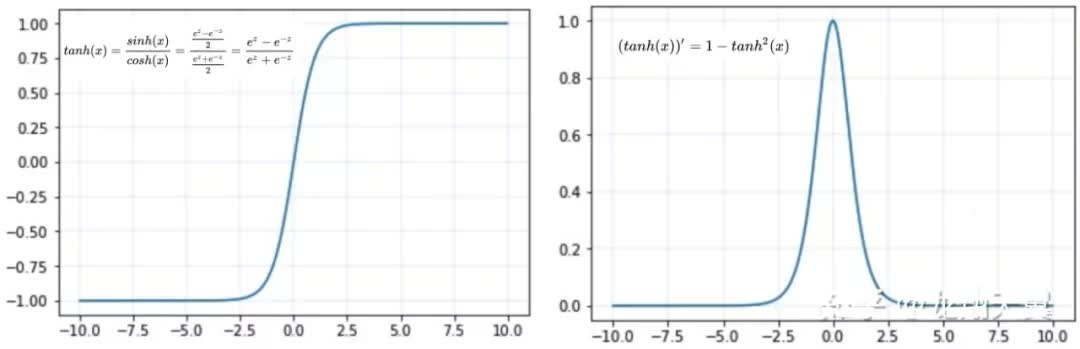
\includegraphics[width = 1\textwidth]{tanh}
\caption{tanh函数及其导数}
\label{piture:9}
\end{figure}

\subsection{整流线性单元(ReLU)}

ReLU函数及其导数如图~\ref{piture:10}~所示。

为了缓解梯度消失问题,ReLU函数被提出来。它简单高效,不涉及指数等运算;而且ReLU激活函数的导数在变动很大的情况下,会远大于于$0$;此外,ReLu激活函数会使神经网络学习效率变高;最后,当$x>0$时,ReLU函数的导数是常数,这有效地解决了梯度弥散现象。这些使得它成为当今最主流的激活函数之一。

\begin{figure}[h]
\centering
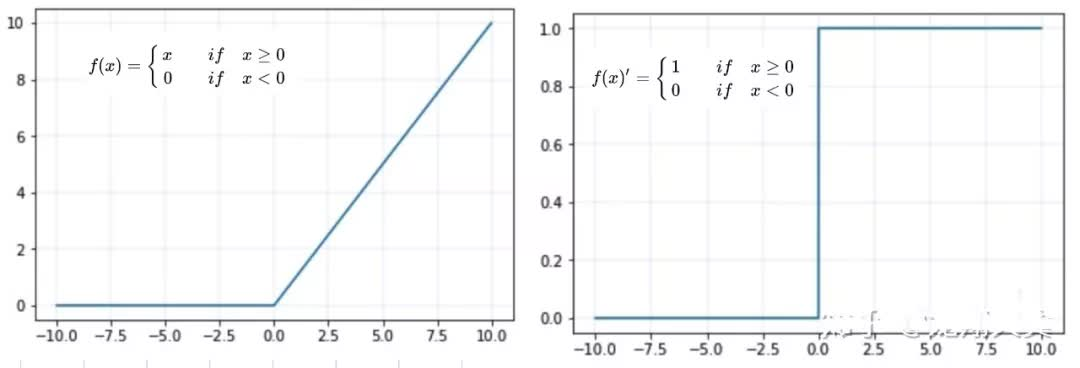
\includegraphics[width = 1\textwidth]{ReLU}
\caption{ReLU函数及其导数}
\label{piture:10}
\end{figure}

\section{正则化}

在机器学习中一切抑制过拟合现象的方法都可以被称作是正则化方法,例如集合学习,数据增强,dropout,修改损失函数等。这里我们主要介绍接下来工作中所用到的通过修改损失函数的正则化方法。

修改损失函数的正则化方法主要有L1正则化(见公式~\ref{eq:9}~),L2正则化(见公式~\ref{eq:10}~)和Smooth L1正则化(见公式~\ref{eq:11}~)。


\begin{align}
L_1(x) ={} & |x| \label{eq:9}\\
L_2(x) ={} & x^2 \label{eq:10}\\
smooth_{L_1}(x) ={} & \left\{
\begin{array}{rl}
\label{eq:11}
0.5x^2 & \text{if } |x| < 1\\
|x|-0.5 & \text{otherwise}
\end{array}\right.
\end{align}

其中$x$为预测值与真值之间的差异。

三个损失函数对$x$的导数分别为:

\begin{align}
\frac{\dif L_1(x)}{\dif x} ={} & \left\{
\begin{array}{rl}
\label{eq:12}
1 & \text{if } x \geqslant 0\\
-1 & \text{otherwise}
\end{array}\right.\\
\frac{\dif L_2(x)}{\dif x} ={} & 2x \label{eq:13}\\
\frac{\dif smooth_{L_1}(x)}{\dif x} ={} & \left\{
\begin{array}{rl}
\label{eq:14}
x & \text{if } |x| < 1\\
\pm 1 & \text{otherwise}
\end{array}\right.
\end{align}

根据公式~\ref{eq:12}~,$L_1$对$X$的导数是常数。这将带来一个问题,那就是训练后期时,真值和预测值之间的差值很小,但$L_1$对$X$的导数仍然不变,导致神经网络难以继续收敛。更致命的是,$L_1$在零点导数不唯一,会影响训练的收敛。

观察公式~\ref{eq:13}~,$L_1$对$X$的导数与$X$呈正相关。所以刚开始训练时真值和预测值之间的差值很大,导致损失函数的梯度也很大,会使得训练不稳定。同时离群点会占据loss的主要部分,造成训练的失败。

而Smooth L1 Loss(公式~\ref{eq:14}~)结合了L1 Loss以及L2 Loss的优点,它既可以较快地收敛,又能降低对离群点的敏感度,使得梯度变化较小,训练不易波动。

\section{本章小结}

本章主要介绍了卷积神经网络的一些信息,为后续研究BlazePose算法打好基础,重点阐述了CNN的组成部件,CNN的反向传播算法,以及激活函数的选择和一些常见的正则化方法。


% Local Variables:
% TeX-master: "../main"
% TeX-engine: xetex
% End:

% !Mode:: "TeX:UTF-8"

\chapter{基于BlazePose的人体姿态估计算法研究}

\section{推理通道}

在推断过程中,采用了detector-tracker设计。流程(见图~\ref{piture:11}~)包括一个轻量级的人体姿态估计检测器,和一个紧随其后的姿态跟踪网络。当目前帧上有人体出现时,使用跟踪网络预测关键点坐标;当跟踪器不能检测出关键点坐标,即没有人出现时,检测器会在下一帧重新启用。

具体来说,模型会使用检测器定位图像的姿态ROI,然后传给跟踪器,预测出33个关键点的坐标。对于视频流来说,检测器只会在第一次出现人脸之前运行。对于检测到人脸之后,会从前一帧的33个关键点中预测出ROI。

\begin{figure}
\centering
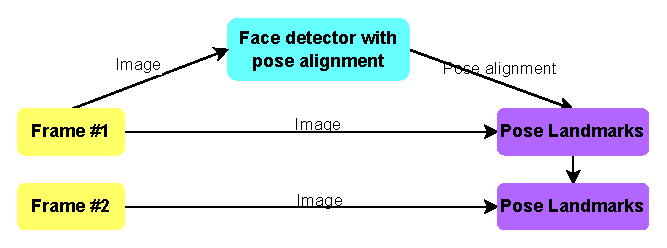
\includegraphics[width=1\linewidth]{Inference_pipeline}
\caption{推理通道}
\label{piture:11}
\end{figure}

\section{神经网络结构}

我们将两种主流的方法,即基于热图和基于回归相结合,如图~\ref{piture:12}~所示。热力图所在的网络层只在训练过程中出现,不包含回归。当训练完成时,热力图相对应的输出层将会被删除,从而降低模型的复杂度,提升模型的轻量化。同时,还使用了堆叠沙漏方法\cite{newell2016stacked},但与之不同的是,本项目同时堆叠了一个encoder-decoder热图网络和一个回归encoder网络。

\begin{figure}
\centering
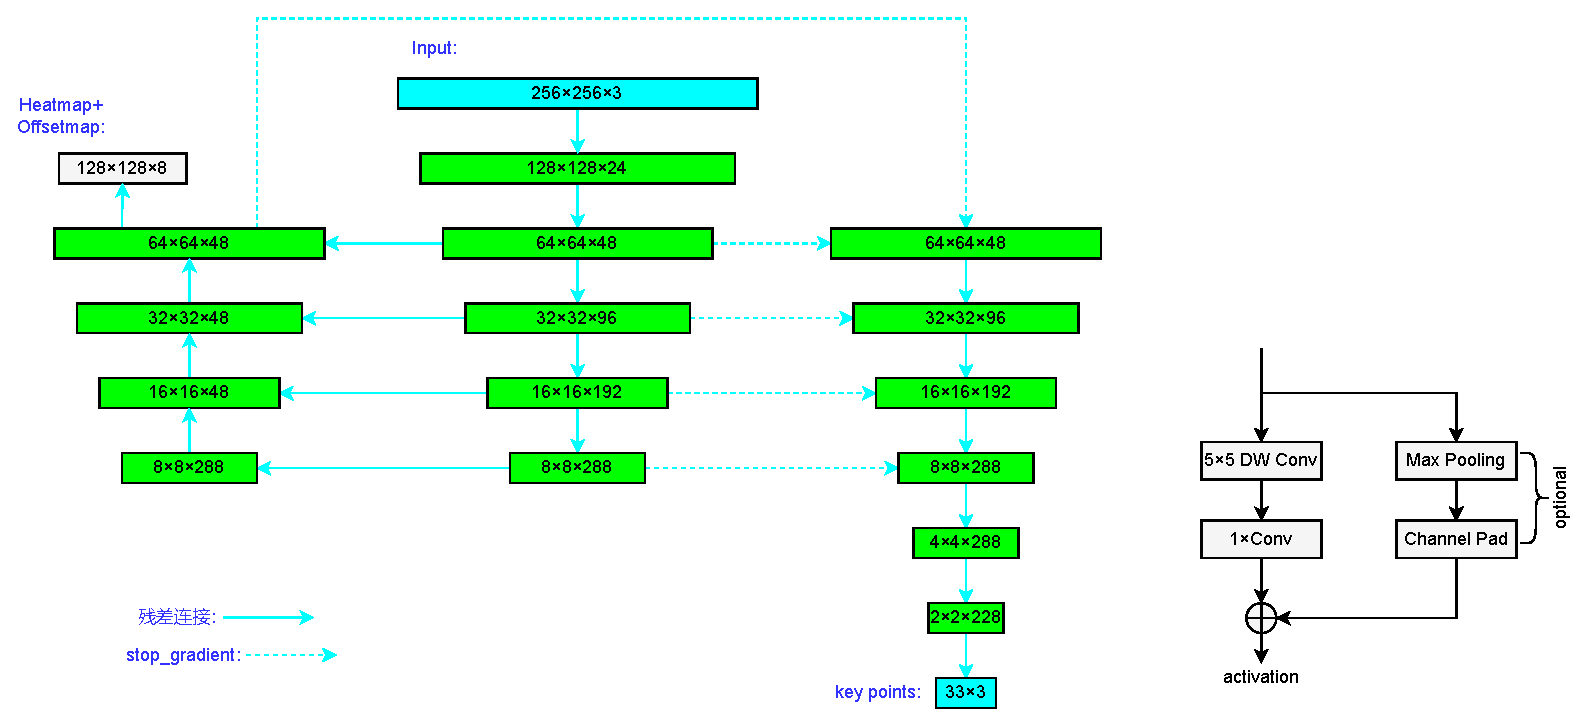
\includegraphics[width=1\linewidth]{model}
\caption{神经网络结构}
\label{piture:12}
\end{figure}

中间上面是输入图片,然后逐步向下,是个bottom-up的过程,每个scale都有向左和向右的横向链接。

左边从下到上,是个top-down的过程,和中间部分有横向链接skip connections,这都和``Hourglass''一样,最上面是``Hourglass''部分输出的heatmap,这个heatmap仅仅用来应用loss监督训练``Hourglass''部分生成中间的embedding特征,在预测以及regression部分都不参与。

右边从上到下整个是regression encoder网络,这部分不参与训练``Hourglass''部分,仅仅用来``后处理''。它每层有对应的输入,其中最上面的第一层输入来自两部分,分别是bottom-up以及top-down的同级分辨率特征(heatmap没有参与过来,也就是砍掉了),最后输出33个关键点信息。

从图~\ref{piture:12}~中可以看出,本项目的模型,充分连接了网络的各个阶段,使其不再孤立,从而平衡了深浅层的特征。不同层次之间存在跨层连接,这样既可以发挥深层网络的特化语义信息,抽象信息;也可以充分发挥浅层网络提取出的细粒度的边缘、颜色、转角、斑块,这些底层的图像信息。图中的实线是残差连接,即可以回传梯度,虚线表示停止回传梯度。这样使得热图的预测准确率和坐标的精度都大大提升。

图~\ref{piture:13}~和图~\ref{piture:14}~分别展示了本项目模型每层的连接关系和每一层的具体实现细节。可以看出网络一共由二十三层,其中Conv7a至Conv11为热力图分支,Conv11为热力图输出,Conv12a至Conv15为回归分支,Conv15为全连接层。中间层激活函数均为Relu,最后一层的激活函数为Sigmoid。

\begin{figure}
\centering
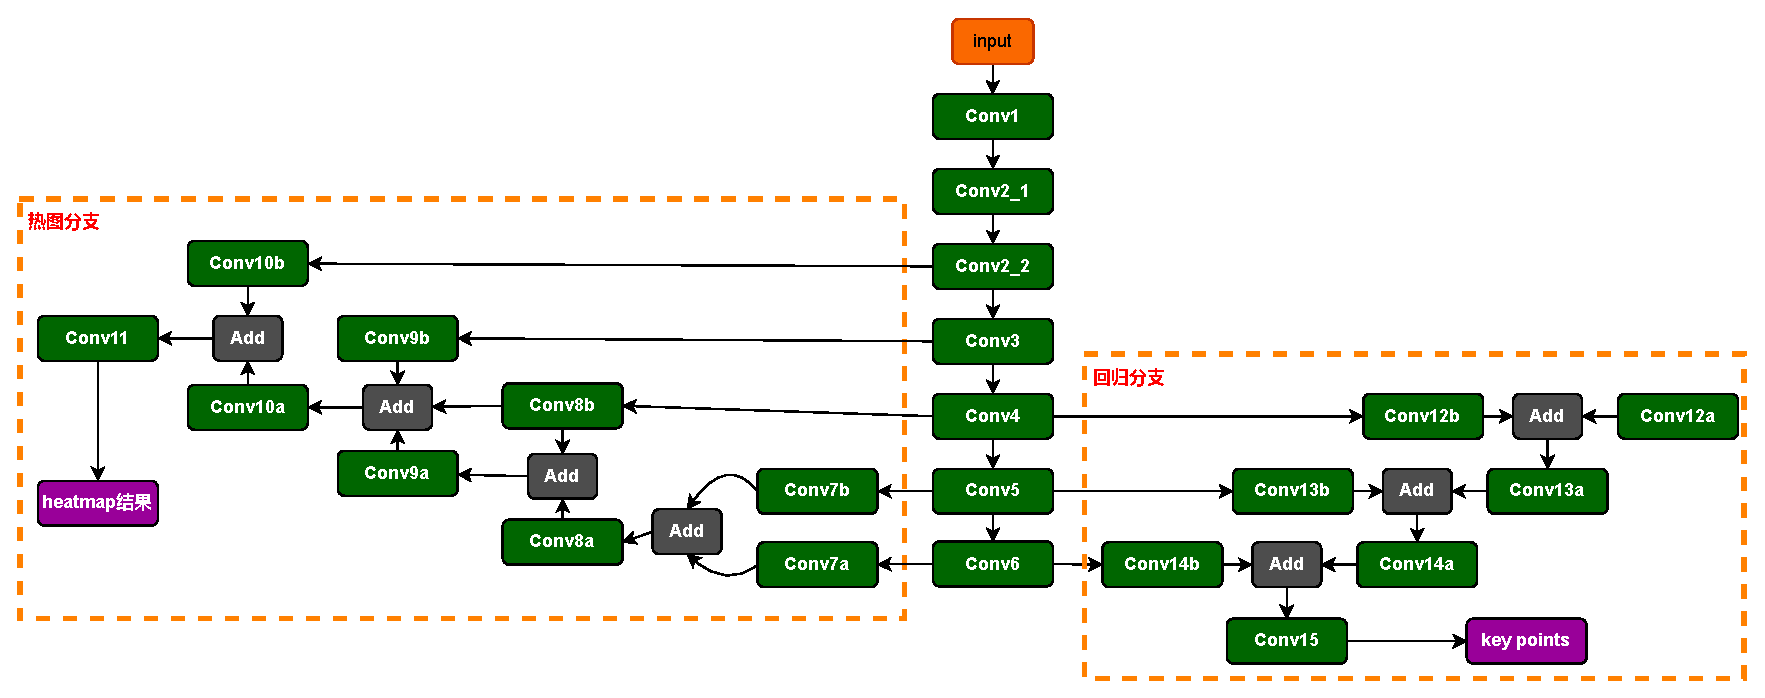
\includegraphics[width=1.1\linewidth]{network-architecture-simple}
\caption{层与层之间的连接关系}
\label{piture:13}
\end{figure}

\begin{figure}[!h]
	\centering
	\begin{sideways}
		\begin{minipage}{\textheight}
			\centering
			\fbox{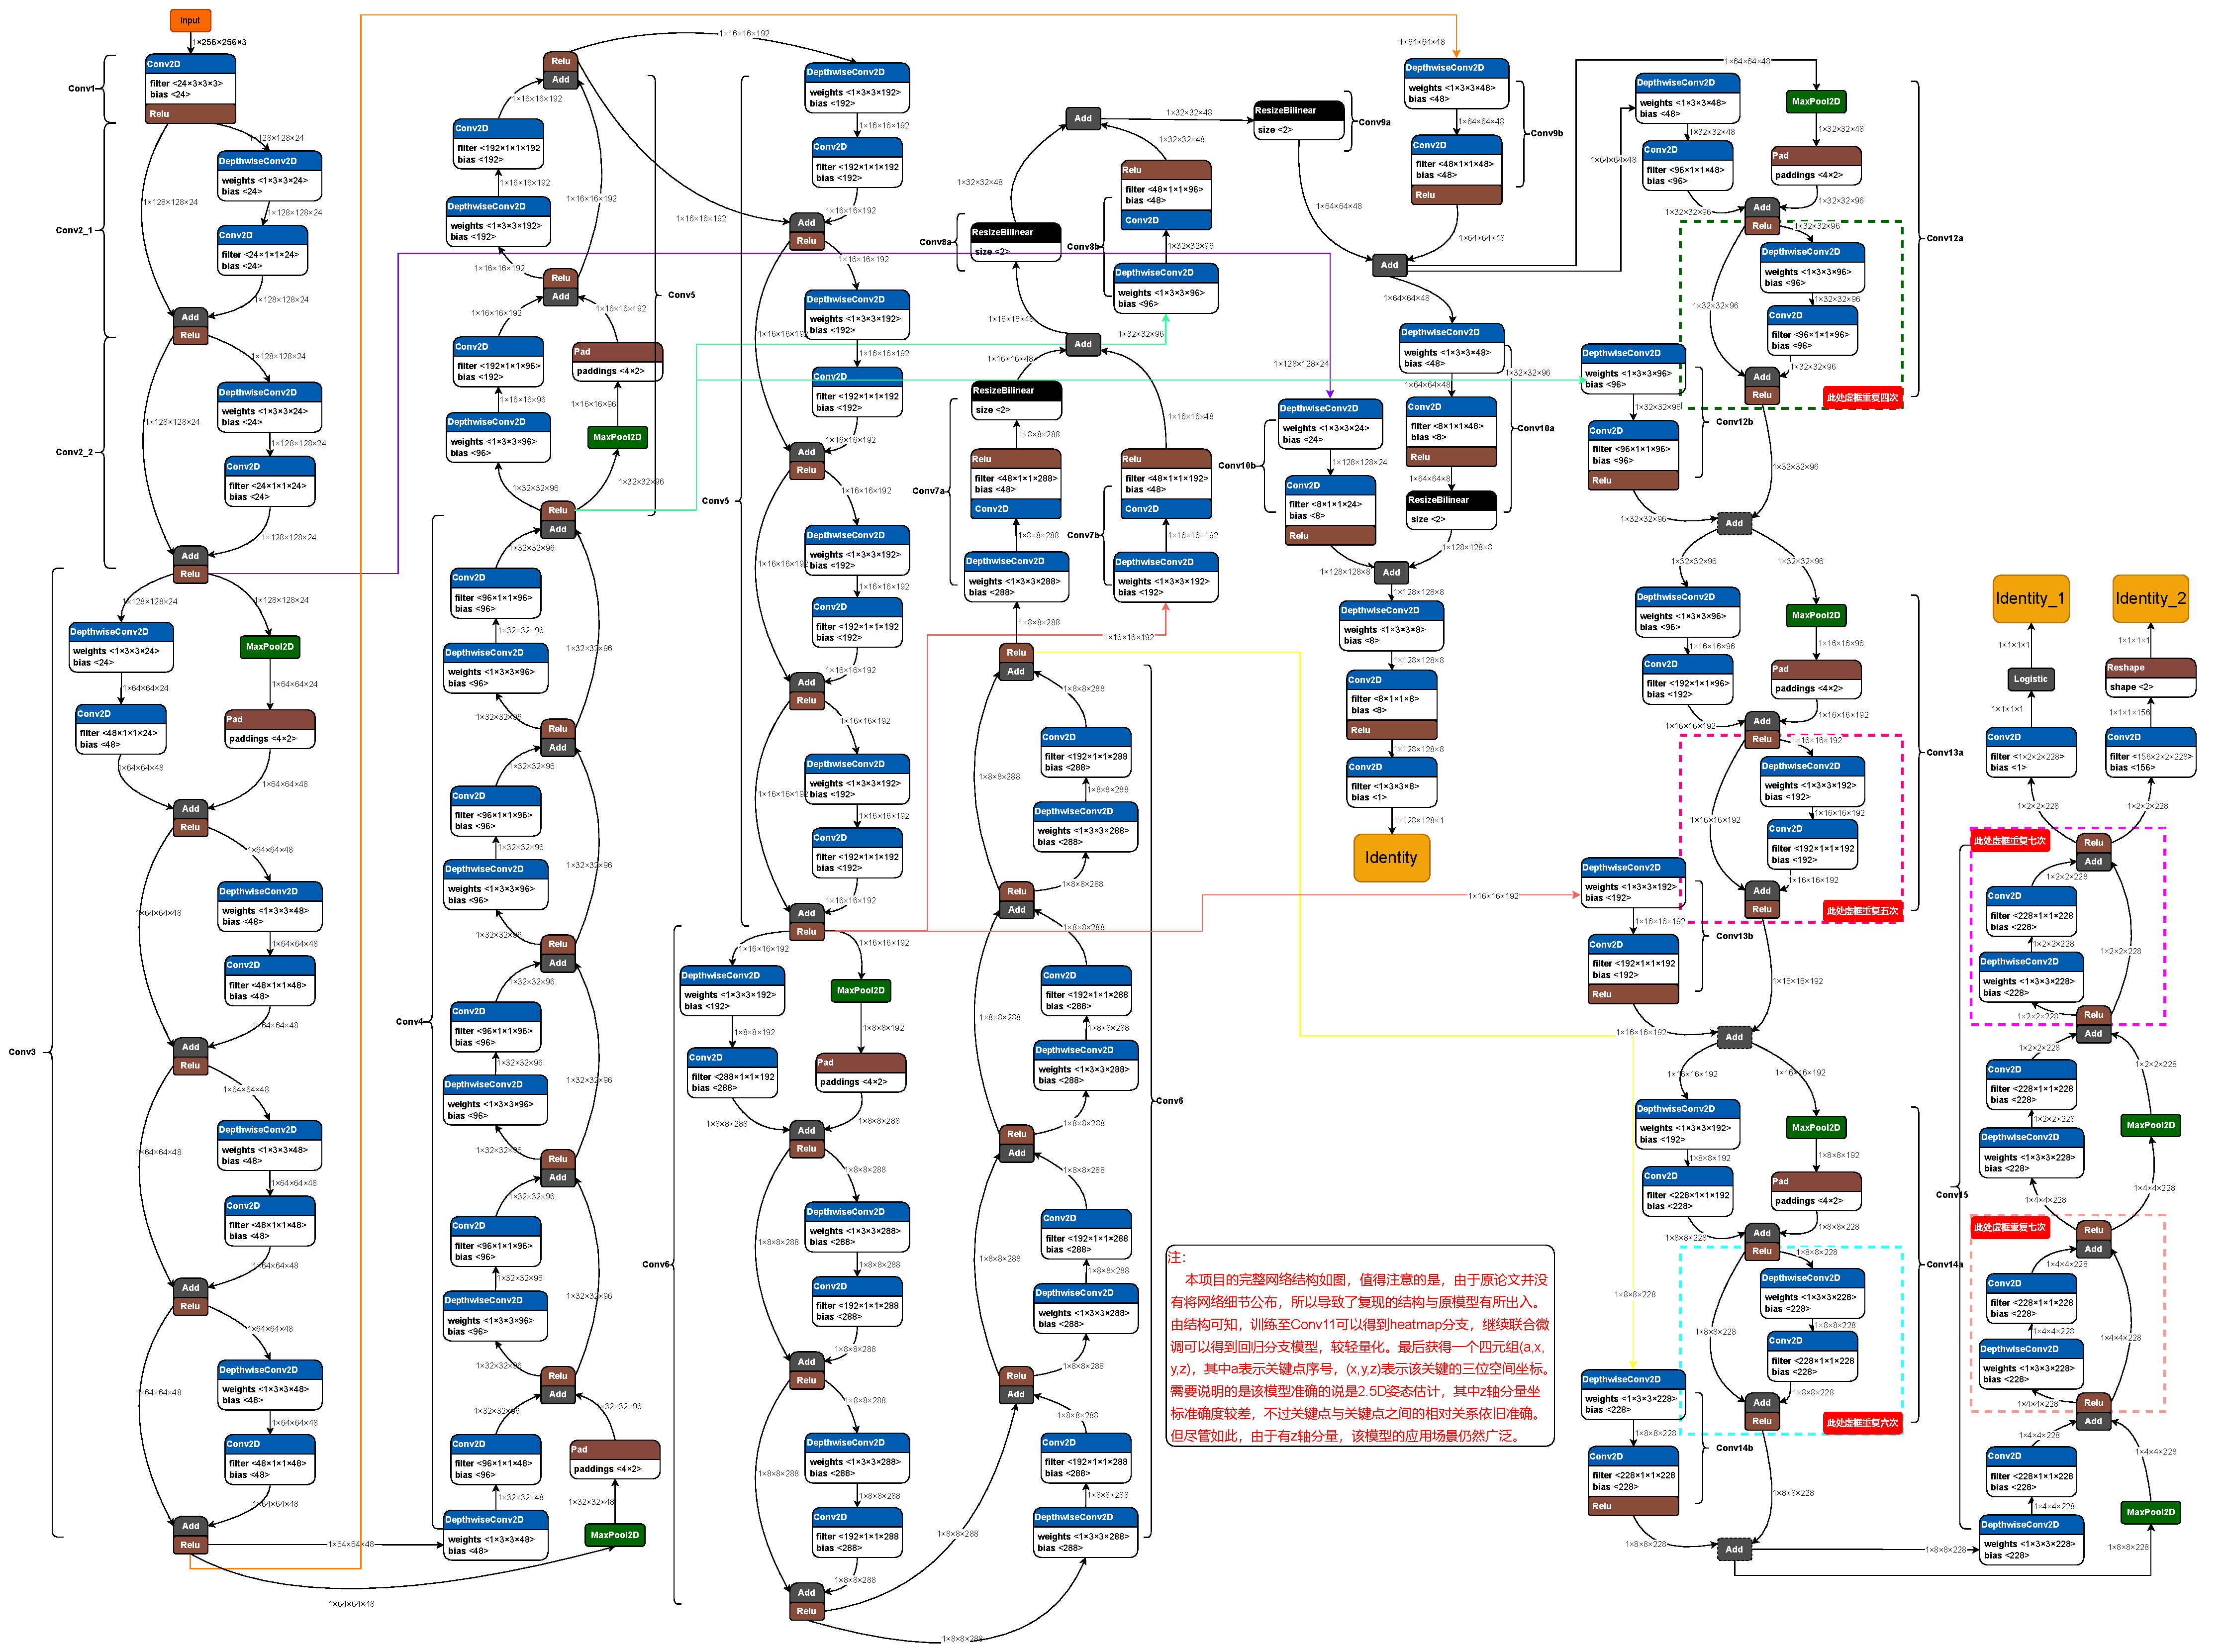
\includegraphics[width=0.9\textwidth]{network-architecture-full}}
			\caption{层与层之间的连接关系和每层的实现细节}
			\label{piture:14}
		\end{minipage}
	\end{sideways}
\end{figure}

\section{人体检测器}

目前主流的人体姿态估计算法在检测人体的后处理步骤中,都是使用的NMS算法,不过NMS对于非刚性物体并不是很友好,尤其是类似与人体这类关节复杂度高的姿势场景。这是因为有大量的,模糊的候选框都满足非最大值抑制的交并比阈值。

因此,本项目摒弃了NMS算法,而采用人脸检测框。这是因为在大多数情况下,人脸较为刚性,是关于躯干的最强信号。因此,我们做出了一个假设,即在单人姿态估计中,人脸是必须要出现的。

该检测器(见图~\ref{piture:15}~)来自谷歌的轻量级BlazeFace模型,它预测了人体两个髋关节的中点作为整个人体的中心,并以此为圆心,画一个能够包含整个人体的最小圆,这就是本项目中的ROI。对于人体倾斜的情况,还预测了人体中心与两个眼睛的中心之连线和铅垂线的夹角,将图像旋转这个夹角即可得到标准的人体图像。

\begin{figure}[htbp]
\centering
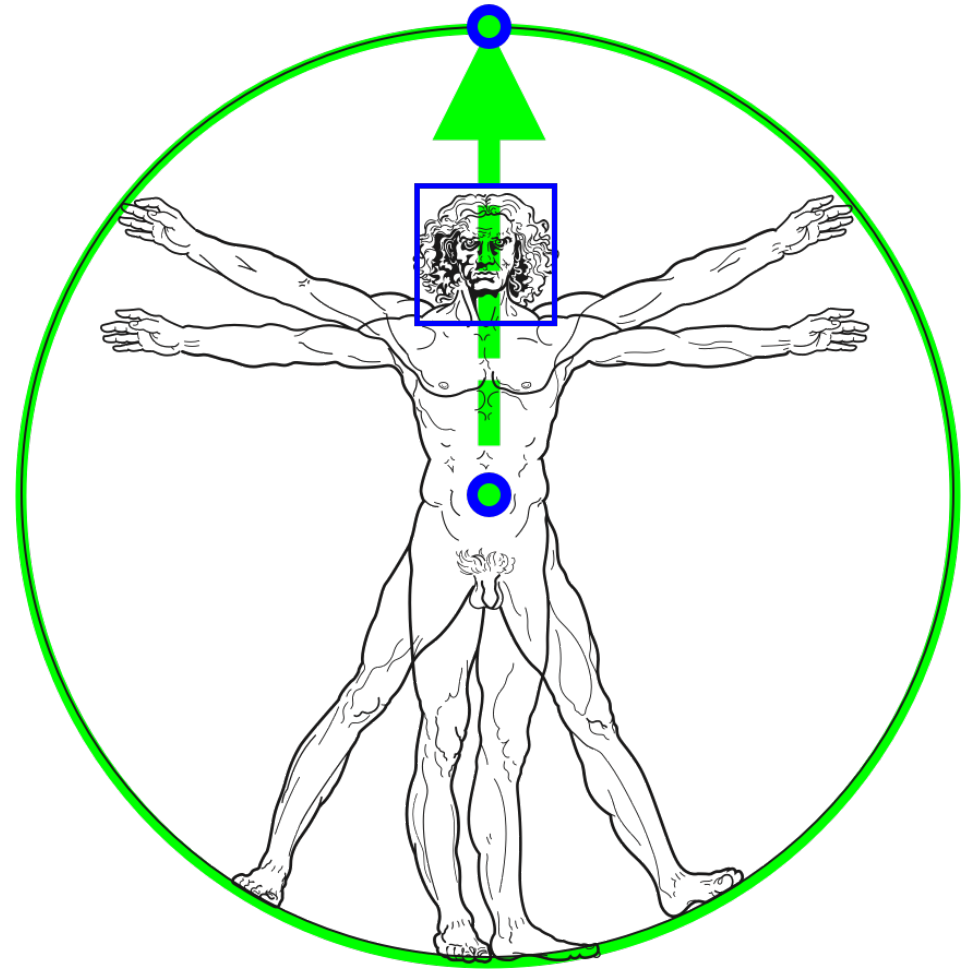
\includegraphics[width=0.6\linewidth]{human}
\caption{从维特鲁威人中受到启发的检测器}
\label{piture:15}
\end{figure}

\section{人体拓扑结构}
我们结合了BlazeFace、BlazePalma和Coco使用的数据集,并研究了他们的并集之超集,提出了人体33个关键点。

和OpenPose\cite{8765346}以及Kinect\cite{zhang2012microsoft}的关键点不同的是,本文在脸部,手部和脚部添加了更多的关键点,用来估计后续模型的ROI。拓扑结构如图 \ref{piture:16}所示。

\begin{figure}
\centering
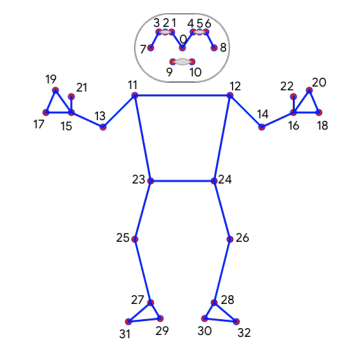
\includegraphics[width=0.6\linewidth]{keypoints}
\caption{33个关键点}
\label{piture:16}
\end{figure}

此外,各个关键点的名称详见附录1\fcolorbox{red}{white}{~\nameref{keypoints}~}。

\section{输入输出}
由复现的网络结构图~\ref{piture:14}~可知,模型的输入是:

视频帧中检测到人的区域。大小是$256\times256\times3$,在垂直身体姿势中以两个髋关节的中部为中心。 通道顺序是RGB。

模型的输出是33对3元组$(X,Y,Z)$,其中33对表示33个关键点,3对分别是关键点在$X,Y,Z$轴上的坐标:

\begin{enumerate}
\item $X,Y$坐标是感兴趣区域的局部坐标,范围为$[0.0,255.0]$;

\item $Z$坐标与$X$和$Y$坐标一样以``图像像素''测量,表示相对于臀部平面的距离。正值表示在臀部的后面,负值表示在臀部和相机之间。这样就可以知晓33个关键点,尤其是手部和腿部的$Z$轴位置,可以充分发挥图像的信息。但$Z$坐标与$X$和$Y$坐标不一样的是,$X$和$Y$坐标通过人工注释获得,而$Z$坐标是通过将合成数据(GHUM模型\cite{xu2020ghum,zanfir2020weakly})拟合到2D模型中,是按比例计算的。
\end{enumerate}

\section{本章小结}
在本章中,我们对BlazePose算法做出了细致的研究,包括其推理通道,神经网络结构,人检测器,关键点模型等等,其中着重介绍了本项目复现出的神经网络结构。

% Local Variables:
% TeX-master: "../main"
% TeX-engine: xetex
% End:

% !Mode:: "TeX:UTF-8"

\chapter{基于BlazePose的训练、姿态识别与模仿}

\section{训练}
如图~\ref{piture:12}~所示,我们将两种主流的方法,即基于热图和基于回归相结合。热力图所在的网络层只在训练过程中出现,不包含回归,即只用右塔来训练中塔和左塔。当训练完成时,热力图相对应的输出层将会被删除,即移除右塔,从而降低模型的复杂度,提升模型的轻量化。

训练步骤主要分如下几步:
\begin{itemize}
\item 训练

\begin{itemize}
\item 下载 LSP 数据集。

\qquad \qquad 手动下载并解压缩数据集至./dataset中。
\item 预训练热图分支。

\qquad \qquad 将config.py中的train\_mode设置train\_mode = 0,然后运行python train.py。

\item 微调联合回归分支。

\qquad \qquad 将config.py中的train\_mode设置为train\_mode = 1,并且设置一个合适的best\_pre\_train值,best\_pre\_train是训练损失下降但测试准确的最佳时期数。然后运行python train.py。
\end{itemize}

\item 测试

\qquad \quad 将config.py中的epoch\_to\_test设置为想要测试的epoch,然后运行python test.py。
\end{itemize}

如图~\ref{piture:17}~所示,最后训练的模型在LSP数据集上的正确率可以达到82.5\%。

\begin{figure}
\centering
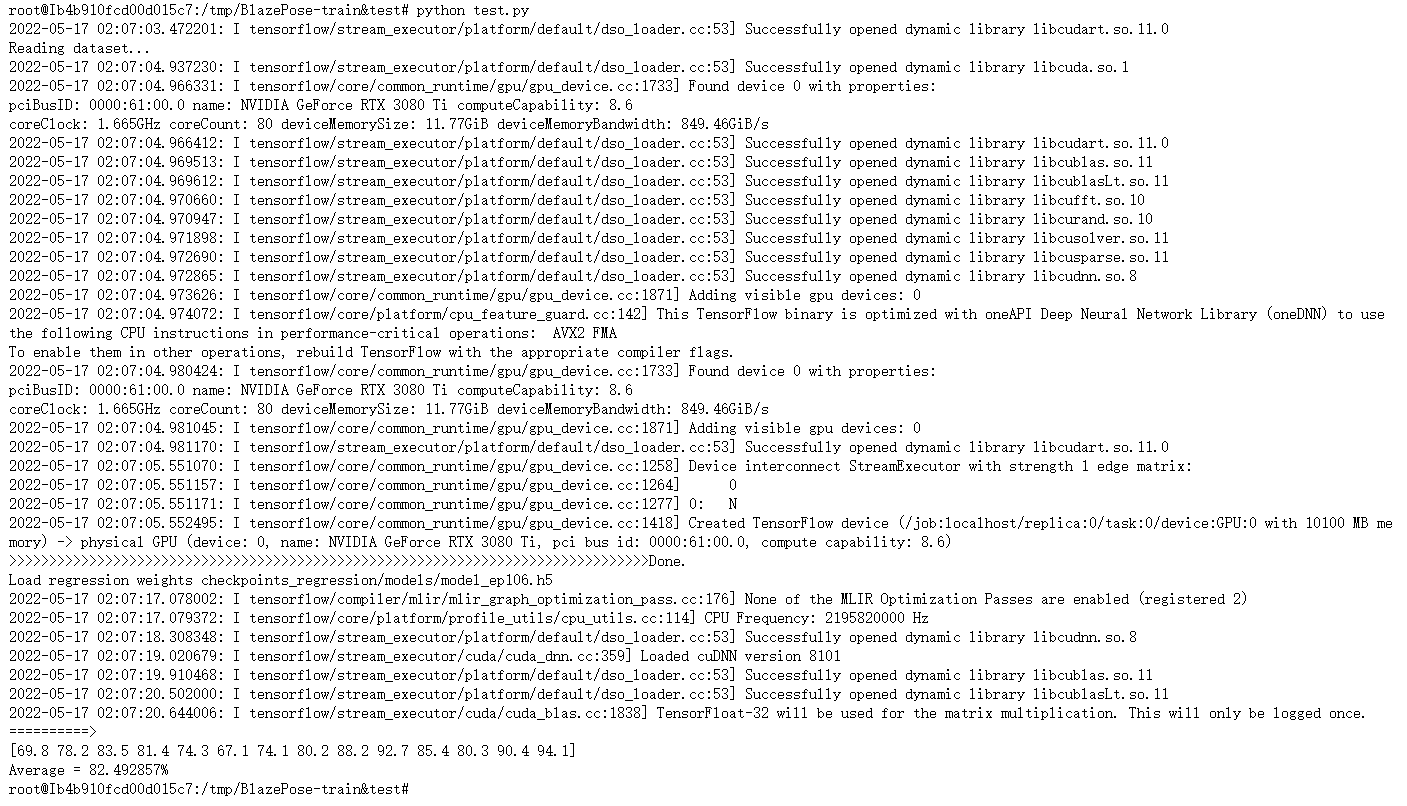
\includegraphics[width=1\linewidth]{acc_result}
\caption{模型在LSP数据集上的正确率}
\label{piture:17}
\end{figure}

\section{性能比较}
同时,本项目还与官方模型以及其它模型做了比较,其中,我们对模型在LSP数据集上做了PCK@0.2的结果对比,见表~\ref{acc}~和图~\ref{piture:27}~。此外,为了验证模型的轻量化,我们还在CPU型号是AMD Ryzen 7 5800H with RadeonGraphics 3.20 GHz上做了帧数对比,见表~\ref{fps}~和图~\ref{piture:28}~。


\begin{table}[htbp]
\caption{LSP数据集上一些模型的PCK}
\label{acc}
\vspace{0.5em}\centering\wuhao
\begin{tabular}{cc}
\toprule[1.5pt]
Model & LSP Dataset(PCK@0.2)  \\
\midrule[1pt]
官方模型(Heavy) & 97.5  \\
官方模型(Full) & 95.7  \\
官方模型(Lite)  & 93.5  \\
AlphaPose ResNet50 & 96.0  \\
Apple Vision  & 88.6  \\
Ours  & 82.5 \\
\bottomrule[1.5pt]
\end{tabular}
\end{table}

\begin{figure}
\centering
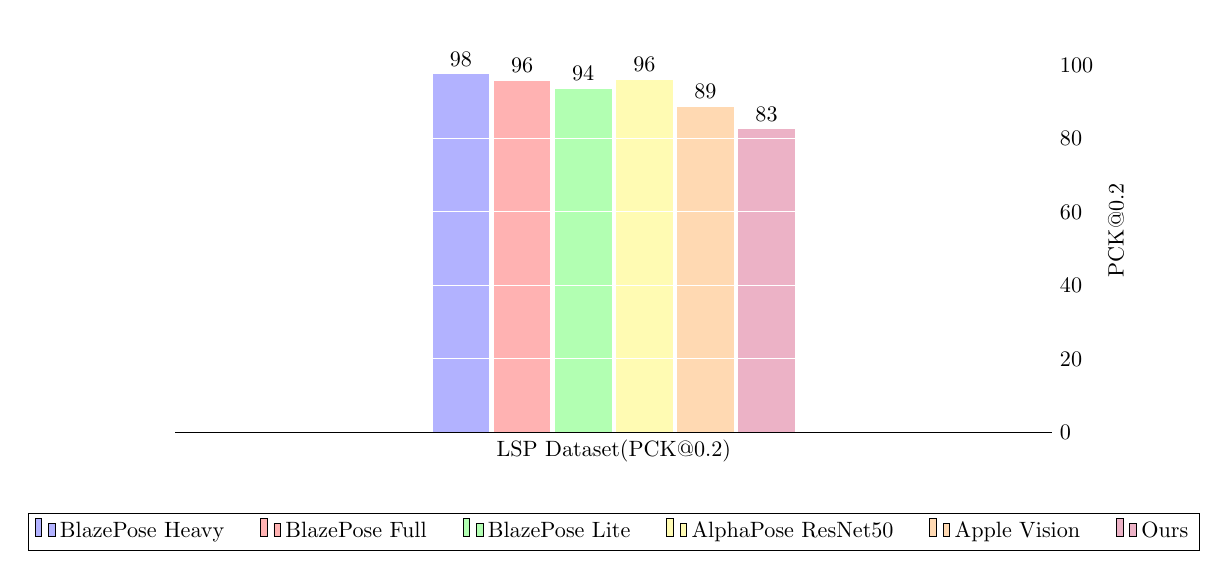
\begin{tikzpicture}[scale = 0.8]
	\begin{axis}[
	ybar, axis on top,
%	title={Cumulative Progress of Works},
	height=8cm, width=15.5cm,
	bar width=0.9cm,
	ymajorgrids, tick align=inside,
	major grid style={draw=white},
	enlarge y limits={value=.1,upper},
	ymin=0, ymax=100,
	axis x line*=bottom,
	axis y line*=right,
	y axis line style={opacity=0},
	tickwidth=0pt,
	enlarge x limits=true,
	legend style={
		at={(0.5,-0.2)},
		anchor=north,
		legend columns=-1,
		/tikz/every even column/.append style={column sep=0.5cm}
	},
	ylabel={PCK@0.2},
	symbolic x coords={
		LSP Dataset(PCK@0.2)},
	xtick=data,
	nodes near coords={
	\pgfmathprintnumber[precision=0]{\pgfplotspointmeta}
	}
    ]
	\addplot [draw=none, fill=blue!30] coordinates { (LSP Dataset(PCK@0.2),97.5) };
	\addplot [draw=none,fill=red!30] coordinates { (LSP Dataset(PCK@0.2),95.7) };
	\addplot [draw=none, fill=green!30] coordinates { (LSP Dataset(PCK@0.2),93.5) };
	\addplot [draw=none, fill=yellow!30] coordinates { (LSP Dataset(PCK@0.2),96.0) };
	\addplot [draw=none, fill=orange!30] coordinates { (LSP Dataset(PCK@0.2),88.6) };
	\addplot [draw=none, fill=purple!30] coordinates { (LSP Dataset(PCK@0.2),82.5) };

	\legend{BlazePose Heavy,BlazePose Full,BlazePose Lite,AlphaPose ResNet50,Apple Vision,Ours}
	\end{axis}
\end{tikzpicture}
\caption{模型在LSP数据集上PCK值的柱状图}
\label{piture:27}
\end{figure}


\begin{table}[htbp]
\caption{一些模型对于视频检测的帧数}
\label{fps}
\vspace{0.5em}\centering\wuhao
\begin{tabularx}{0.7\textwidth}{cX}
\toprule[1.5pt]
Model & FPS(AMD Ryzen 7 5800H with Radeon Graphics 3.20 GHz)  \\
\midrule[1pt]
官方模型(Heavy) & 38  \\
官方模型(Full) & 32  \\
官方模型(Lite) & 25  \\
OpenPose  & 6  \\
Ours  & 29 \\
\bottomrule[1.5pt]
\end{tabularx}
\end{table}

\begin{figure}
\centering
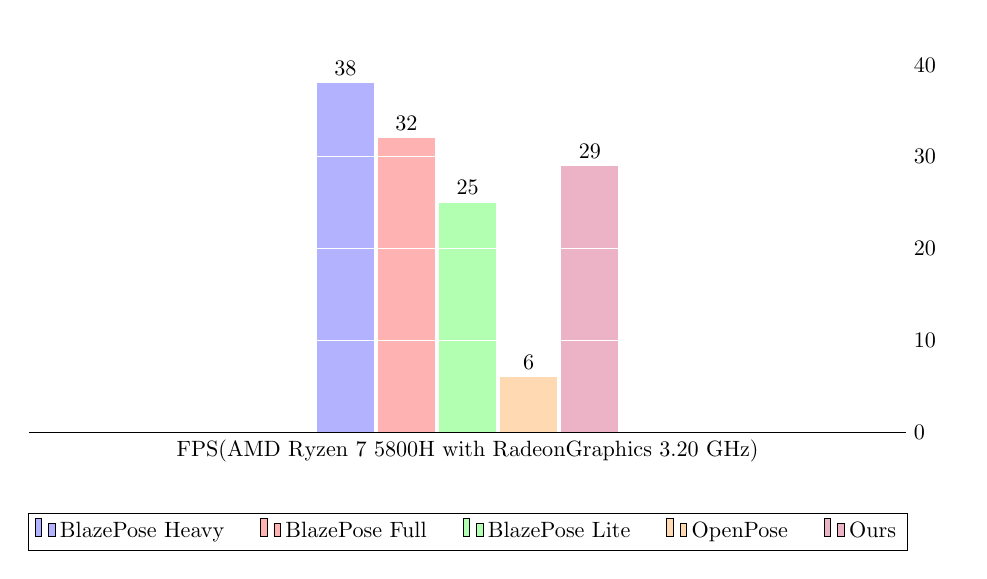
\begin{tikzpicture}[scale = 0.8]
\centering
	\begin{axis}[
	ybar, axis on top,
%	title={Cumulative Progress of Works},
	height=8cm, width=15.5cm,
	bar width=0.9cm,
	ymajorgrids, tick align=inside,
	major grid style={draw=white},
	enlarge y limits={value=.1,upper},
	ymin=0, ymax=40,
	axis x line*=bottom,
	axis y line*=right,
	y axis line style={opacity=0},
	tickwidth=0pt,
	enlarge x limits=true,
	legend style={
		at={(0.5,-0.2)},
		anchor=north,
		legend columns=-1,
		/tikz/every even column/.append style={column sep=0.5cm}
	},
	ylabel={帧数值},
	symbolic x coords={FPS(AMD Ryzen 7 5800H with RadeonGraphics 3.20 GHz)},
	xtick=data,
	nodes near coords={
	\pgfmathprintnumber[precision=0]{\pgfplotspointmeta}
	}
    ]
	\addplot [draw=none, fill=blue!30] coordinates {(FPS(AMD Ryzen 7 5800H with RadeonGraphics 3.20 GHz),38) };
	\addplot [draw=none,fill=red!30] coordinates {(FPS(AMD Ryzen 7 5800H with RadeonGraphics 3.20 GHz),32) };
	\addplot [draw=none, fill=green!30] coordinates {(FPS(AMD Ryzen 7 5800H with RadeonGraphics 3.20 GHz),25) };
	\addplot [draw=none, fill=orange!30] coordinates {(FPS(AMD Ryzen 7 5800H with RadeonGraphics 3.20 GHz),6) };
	\addplot [draw=none, fill=purple!30] coordinates {(FPS(AMD Ryzen 7 5800H with RadeonGraphics 3.20 GHz),29) };

	\legend{BlazePose Heavy,BlazePose Full,BlazePose Lite,OpenPose,Ours}
	\end{axis}
\end{tikzpicture}
\caption{模型在CPU上帧数的柱状图}
\label{piture:28}
\end{figure}


从表中数据我们可以看出,虽然我们根据官方Full版本复现的模型在准确度方面与原版有着差距,但是也已经达到了可以应用的程度,并且在轻量化方面也做到了媲美原版。

\section{API}
对于模型的部署,本项目没有设计函数,而是将我们的模型替换官方模型,再用MediaPipe库调用我们的模型,所以在部署模型之前,我们有必要介绍一下API。

\begin{enumerate}
\item STATIC\_IMAGE\_MODE

\qquad \quad 默认值是false,可以选择true。如果选择false,合适于检测视频,如图~\ref{piture:11}~所示,检测器只会在第一次出现人脸之前运行,当检测到人脸之后,检测器定位图像的姿态ROI,然后传给跟踪器,预测出33个关键点的坐标。对于检测到人脸之后,会从前一帧的33个关键点中预测出ROI,而不会再次启用检测器;对于true,就是每一帧都会启用检测器,这会大大加大CPU的负担。

\item MODEL\_COMPLEXITY

\qquad \quad 可选值是$0,1,2$分别对于着官方模型的Lite、Full和Heavy版本。由于我们复现的是官方的Full模型,所以在此我们只能选择$1$,值得说明的是,该参数的默认值就是$1$。

\item UPPER\_BODY\_ONLY

\qquad \quad 设置为true表示识别出全身33个关键点;设置为false表示识别出上半身的25个关键点。

\item SMOOTH\_LANDMARKS

\qquad \quad 设置为true,将会平滑关键点,从而减少抖动。但如果检测单张图像,即STATIC\_IMAGE\_MODE也设置为true,则忽略该参数。

\item MIN\_DETECTION\_CONFIDENCE

\qquad \quad 置信度阈值,范围是$[0.0,1.0]$,默认设置为0.5。在人体检测器中,如果该像素点的置信度超过了设定的阈值,则认为该像素点为人体。

\item MIN\_TRACKING\_CONFIDENCE

\qquad \quad 追踪阈值,范围是$[0.0,1.0]$,默认设置为0.5。在追踪器中,如果超过该阈值,则表示成功检测到33个关键点,否则将会在下一帧中调用人体检测器。但如果STATIC\_IMAGE\_MODE也设置为true,即检测单张图像,则忽略该参数。
\end{enumerate}

\section{基于BlazePose的姿态识别}

\subsection{电脑端的姿态识别}
这里对于在电脑端部署模型,本项目并没有另外设计函数,本项目采取的方法是将训练好的.h5模型用tensorflow工具转换成.tflite模型,再将其替换谷歌官方的MediaPipe库中的模型,从而可以直接调用谷歌MediaPipe库的方法来测试我们的模型。

\subsubsection{检测人物并蒙版抠图}
该部分主要将图像中的人物检测出来并蒙版抠图,主要是为后续的关键点检测提供ROI。

值得注意的一点是,我们需要使用opencv库提供的cvtColor颜色空间转换函数,将读入的BGR格式转换成matplotlib可输出的RGB格式。

实现方法主要是使用了Selfie Segmentation工具包,该工具包会给出每个像素点是人体一部分的概率,我们设定一个阈值(0.5),如果概率小于阈值,我们不输出该像素点;如果概率大于该阈值,我们则认为该像素点是人体的一部分,输出该像素点。

效果如图~\ref{picture:17}~所示。

\begin{figure}
\centering
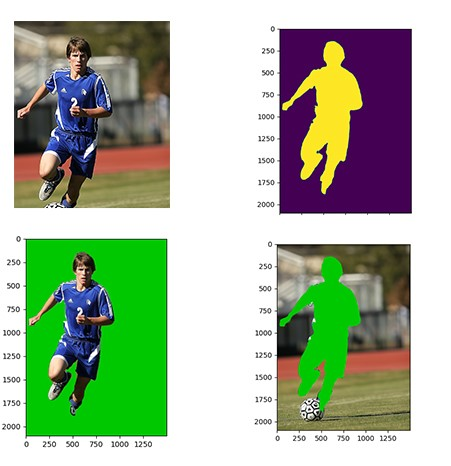
\includegraphics[width=0.7\linewidth]{mask}
\caption{左上为原图,后上是蒙版\\左下是前景人像,右下为抠掉前景人像的背景}
\label{picture:17}
\end{figure}

\subsubsection{单张图片检测}
本部分完成的是对于单张图片的BlazePose关键点检测。函数主要调用了MediaPipe库。

同时由于单张图片的检测会使得模型第一次检测到人体,因此一定会调用人检测器定位ROI。

我们会获得33个关键点的各自像素坐标,然后将该关键点染色并连接

对于各个关键点用不同的颜色加以区分。

主要代码如下:
\begin{python}
for i in range(33):
  h, w = img.shape[0], img.shape[1]
  
  cx = int(results.pose_landmarks.landmark[i].x * w)
  cy = int(results.pose_landmarks.landmark[i].y * h)
  cz = results.pose_landmarks.landmark[i].z

  radius = 10

  if i == 0: # 鼻
    img = cv2.circle(img,(cx,cy), radius, (0,0,255), -1)
  elif i in [11,12]: # 肩
    img = cv2.circle(img,(cx,cy), radius, (223,155,6), -1)
  elif i in [23,24]: # 髋
    img = cv2.circle(img,(cx,cy), radius, (1,240,255), -1)
  elif i in [13,14]: # 肘
    img = cv2.circle(img,(cx,cy), radius, (140,47,240), -1)
  elif i in [25,26]: # 膝
    img = cv2.circle(img,(cx,cy), radius, (0,0,255), -1)
  elif i in [15,16,27,28]: # 手腕、脚腕
    img = cv2.circle(img,(cx,cy), radius, (223,155,60), -1)
  elif i in [17,19,21]: # 左手
    img = cv2.circle(img,(cx,cy), radius, (94,218,121), -1)
  elif i in [18,20,22]: # 右手
    img = cv2.circle(img,(cx,cy), radius, (16,144,247), -1)
  elif i in [27,29,31]: # 左脚
    img = cv2.circle(img,(cx,cy), radius, (29,123,243), -1)
  elif i in [28,30,32]: # 右脚
    img = cv2.circle(img,(cx,cy), radius, (193,182,255), -1)
  elif i in [9,10]: # 嘴
    img = cv2.circle(img,(cx,cy), radius, (205,235,255), -1)
  elif i in [1,2,3,4,5,6,7,8]: # 眼、脸颊
    img = cv2.circle(img,(cx,cy), radius, (94,218,121), -1)
  else: # 其它关键点
    img = cv2.circle(img,(cx,cy), radius, (0,255,0), -1)

look_img(img)
\end{python}

结果如图~\ref{picture:18}~所示。

\begin{figure}
\centering
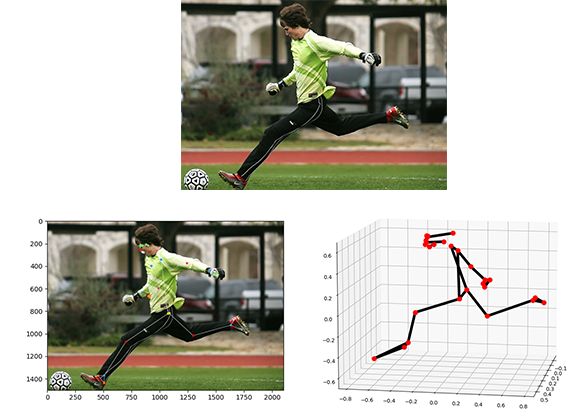
\includegraphics[width=0.7\linewidth]{Single}
\caption{上方为原图,左下为关键点骨架图,右下为三维图}
\label{picture:18}
\end{figure}

\subsubsection{在线摄像头检测}

本部分主要是使用BlazePose模型对摄像头实时检测。

主要代码和单张图片类似,不过输入换成了摄像头。

另外值得说明的是,对于连续视频流,我们只会在第一个人体出来的帧之前帧调用人检测器,此后的帧只会在上一帧的33个关键点中预测出当前帧的ROI。从而使得模型更加轻量化,更加实时化。

结果如图~\ref{picture:19}~所示。

\begin{figure}
\centering
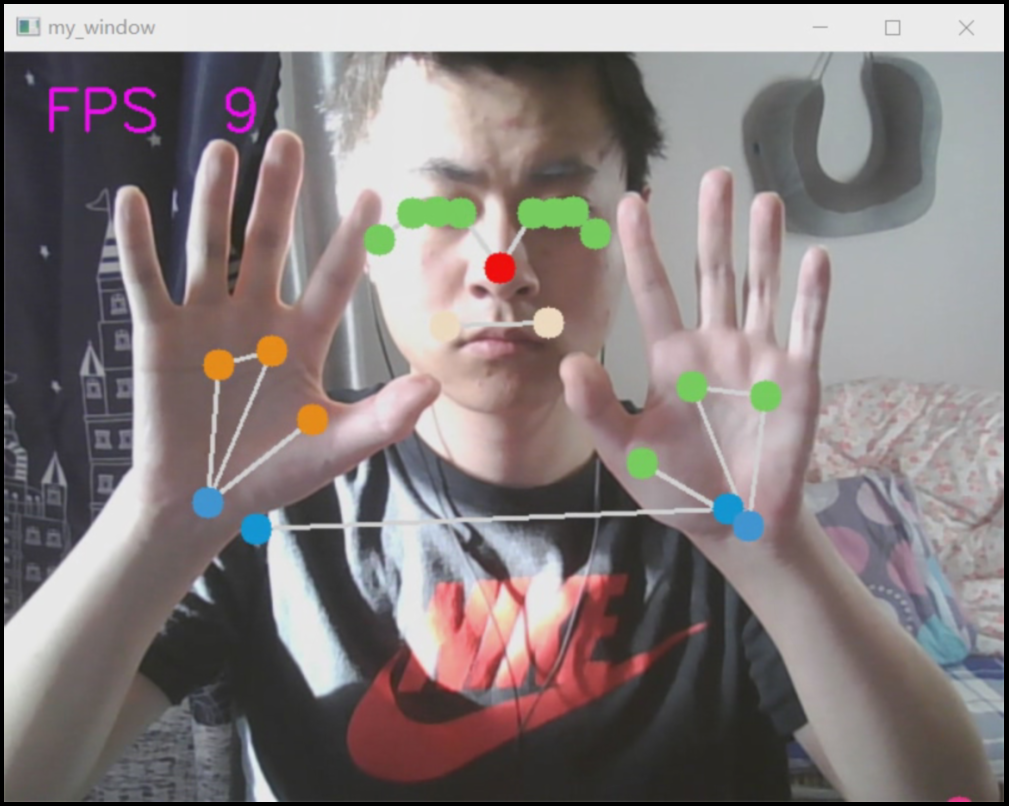
\includegraphics[width=0.7\linewidth]{camera}
\caption{摄像头实时检测截图}
\label{picture:19}
\end{figure}

\subsubsection{离线视频检测}

本部分主要是使用BlazePose模型对离线视频检测。

本部分核心代码和实时检测摄像头相同,主要加了一个生成视频的函数。这样使得输入输出均为视频。

结果如图~\ref{picture:20}~所示。

\begin{figure}[!h]
\setlength{\subfigcapskip}{-1bp}
\centering
\begin{minipage}{\textwidth}
\centering
\subfigure[原视频截图]{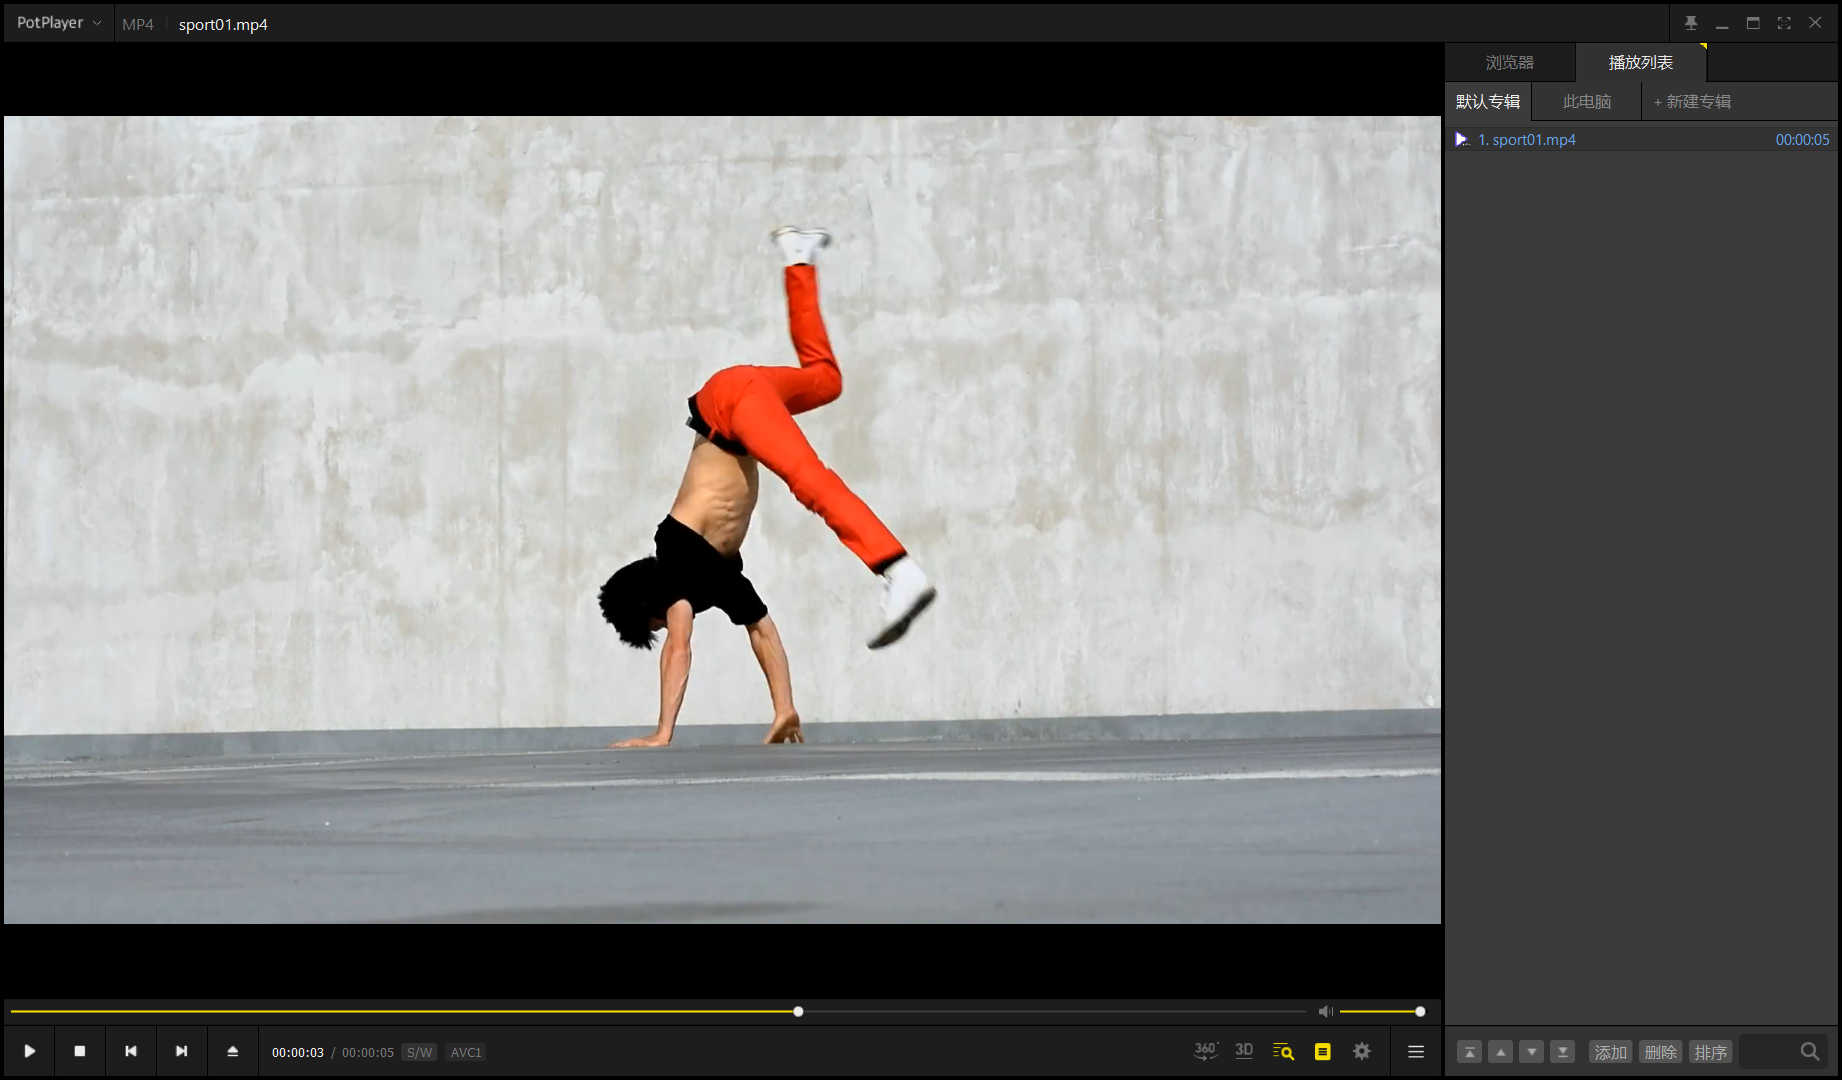
\includegraphics[width=0.45\textwidth]{video1}}
\hspace{2em}
\subfigure[输出视频截图]{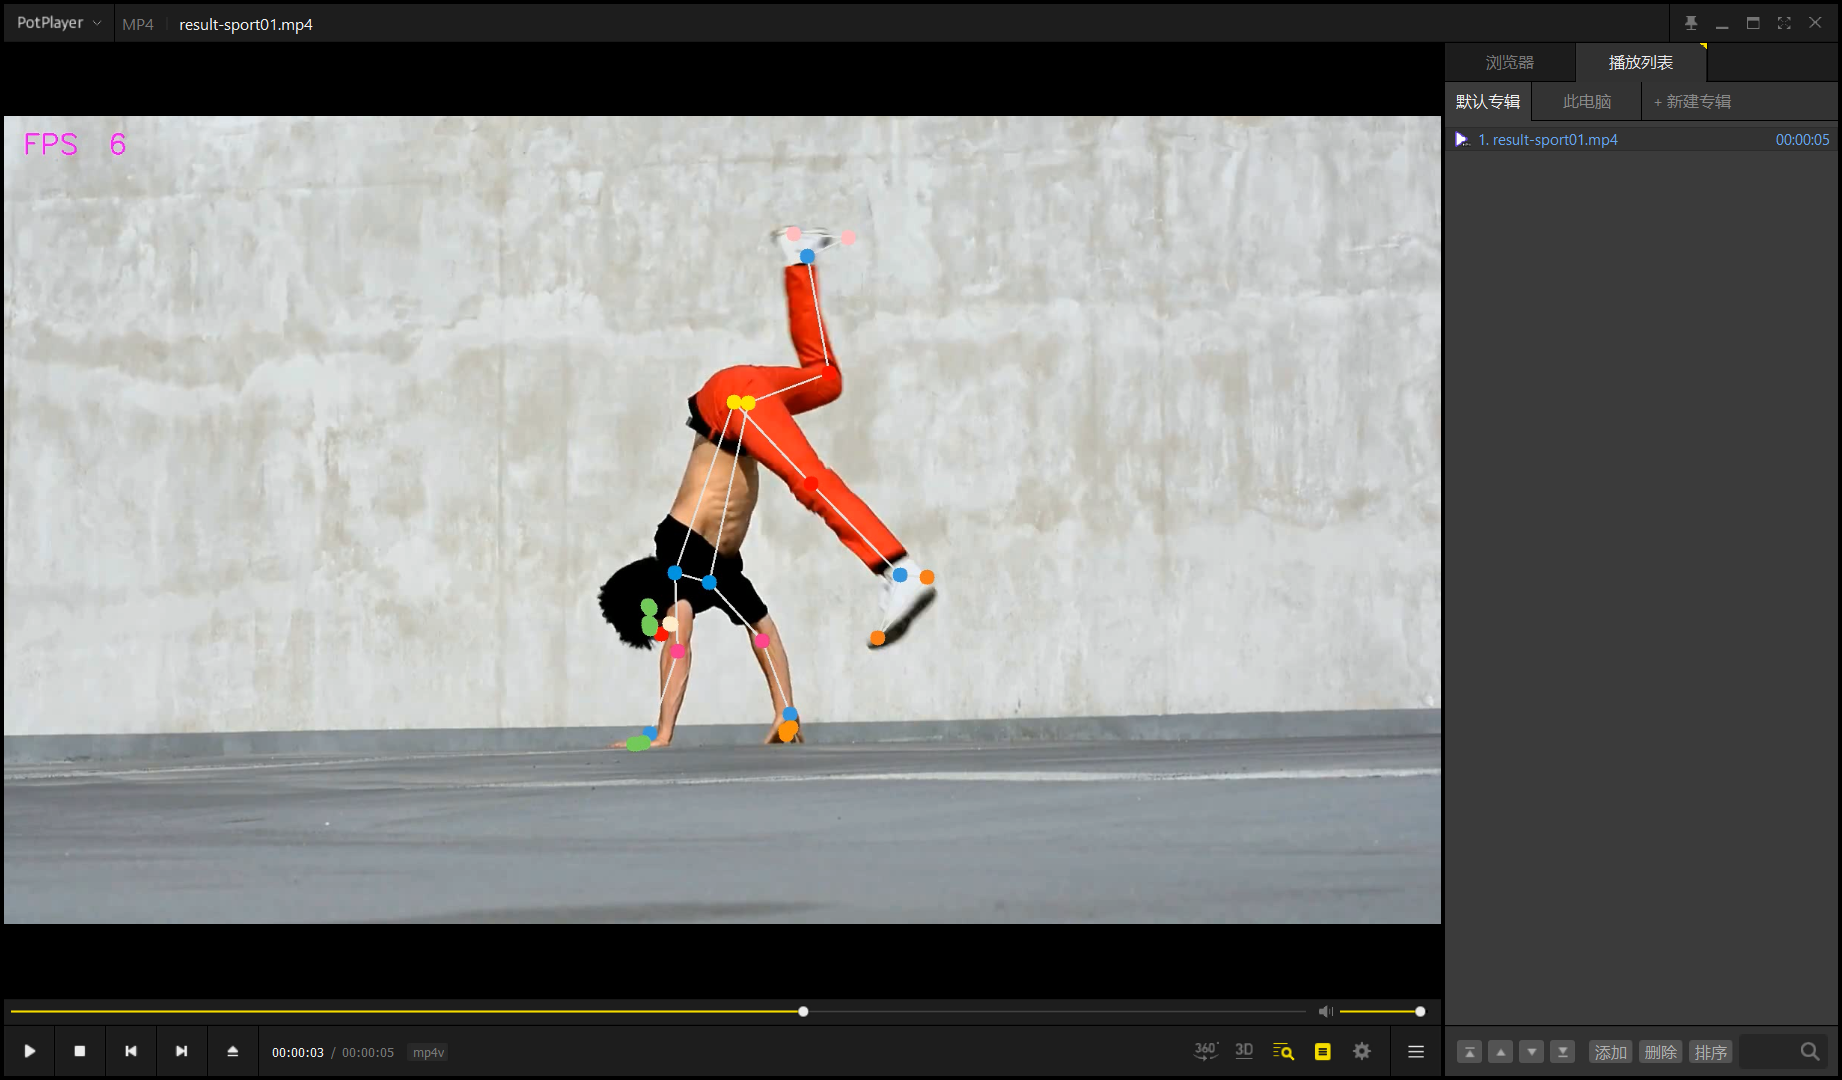
\includegraphics[width=0.45\textwidth]{video2}}
\end{minipage}
\vspace{0.2em}
\caption{离线视频检测}
\label{picture:20}
\end{figure}


\subsection{移动端的姿态识别}

对于移动端的部署,本项目采用腾讯的TNN\footnote{\href{https://github.com/Tencent/TNN}{https://github.com/Tencent/TNN}}轻量化框架,其提供了各种框架模型 (如 TensorFlow、PyTorch、Caffe等) 转化为TNN模型文件的脚本,还有丰富的demo可供学习。其架构图如图~\ref{picture:22}~所示。

\begin{figure}
\centering
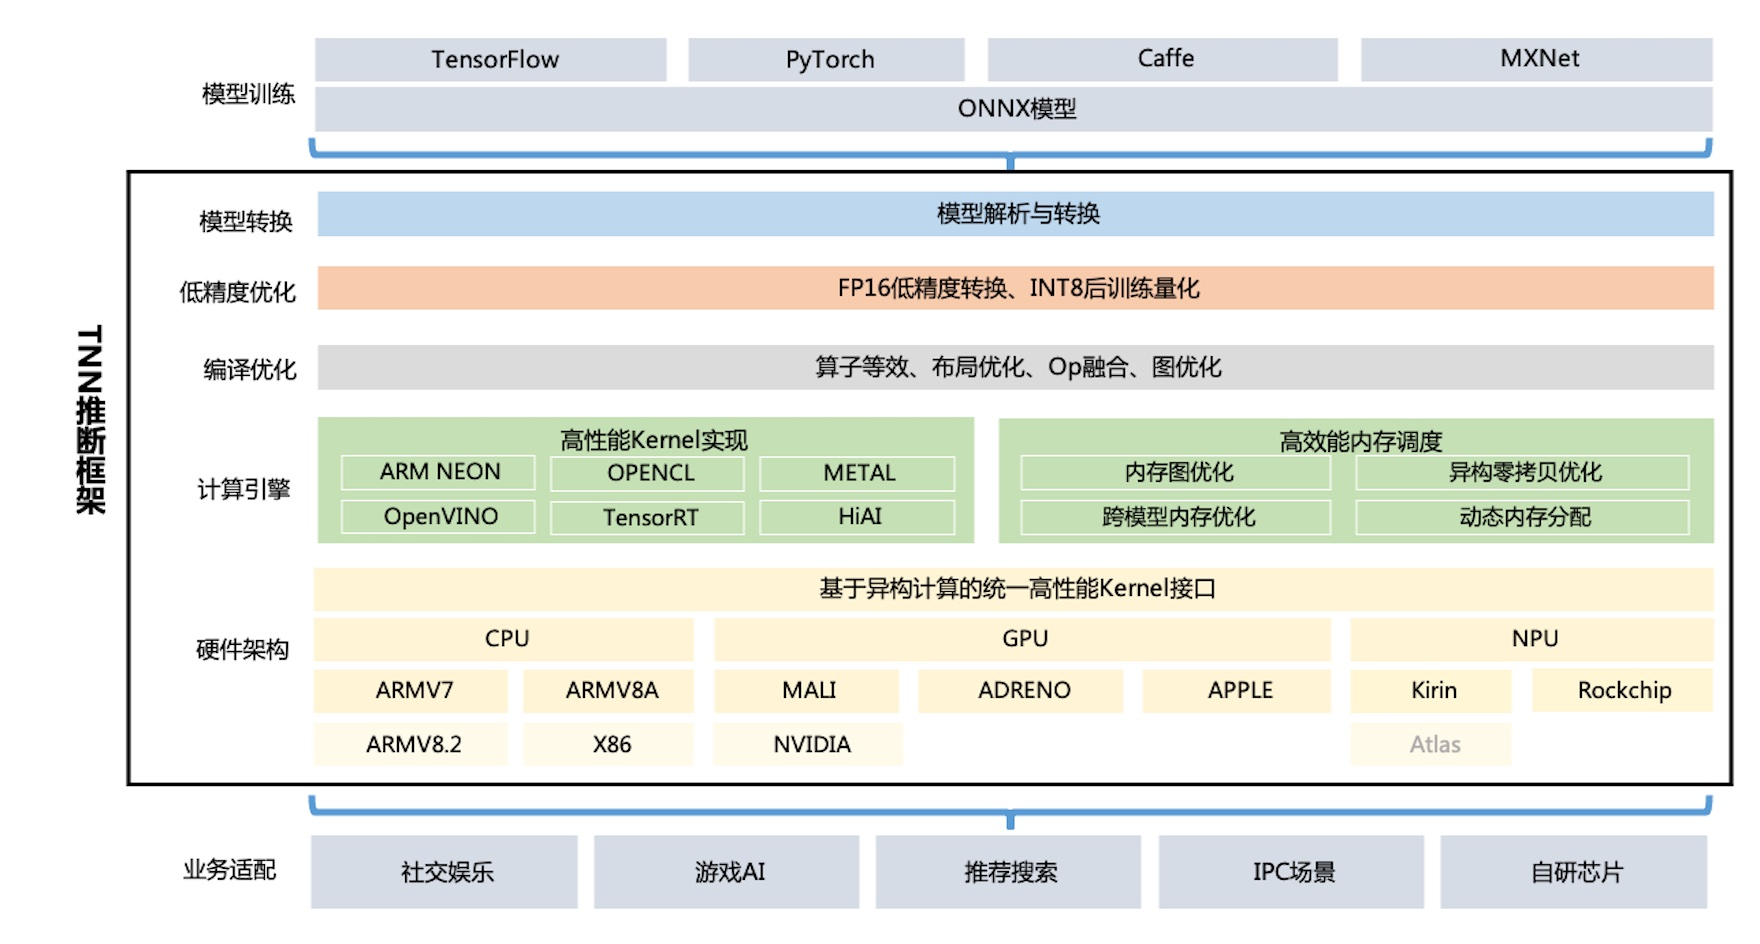
\includegraphics[width=0.7\linewidth]{architecture}
\caption{TNN架构图}
\label{picture:22}
\end{figure}

首先我们使用TNN官方的转换脚本\footnote{\href{https://github.com/Tencent/TNN/blob/master/doc/cn/user/convert.md}{https://github.com/Tencent/TNN/blob/master/doc/cn/user/convert.md}}将我们的.tflite模型转换成.tnn模型

然后编译TNN引擎,我们选择了arm和OpenCL这两个平台。对于这两个平台,TNN都有极其方便的脚本\footnote{\href{https://github.com/Tencent/TNN/blob/master/doc/cn/user/compile.md}{https://github.com/Tencent/TNN/blob/master/doc/cn/user/compile.md}}。

最后,我们构建了一个调用编译好的TNN引擎进行推理的应用程序,从而在手机端部署了我们的模型。

移动端app对于摄像头实时检测的结果截图如图~\ref{picture:23}~所示。

\begin{figure}[!h]
\setlength{\subfigcapskip}{-1bp}
\centering
\begin{minipage}{\textwidth}
\centering
\subfigure[主界面截图]{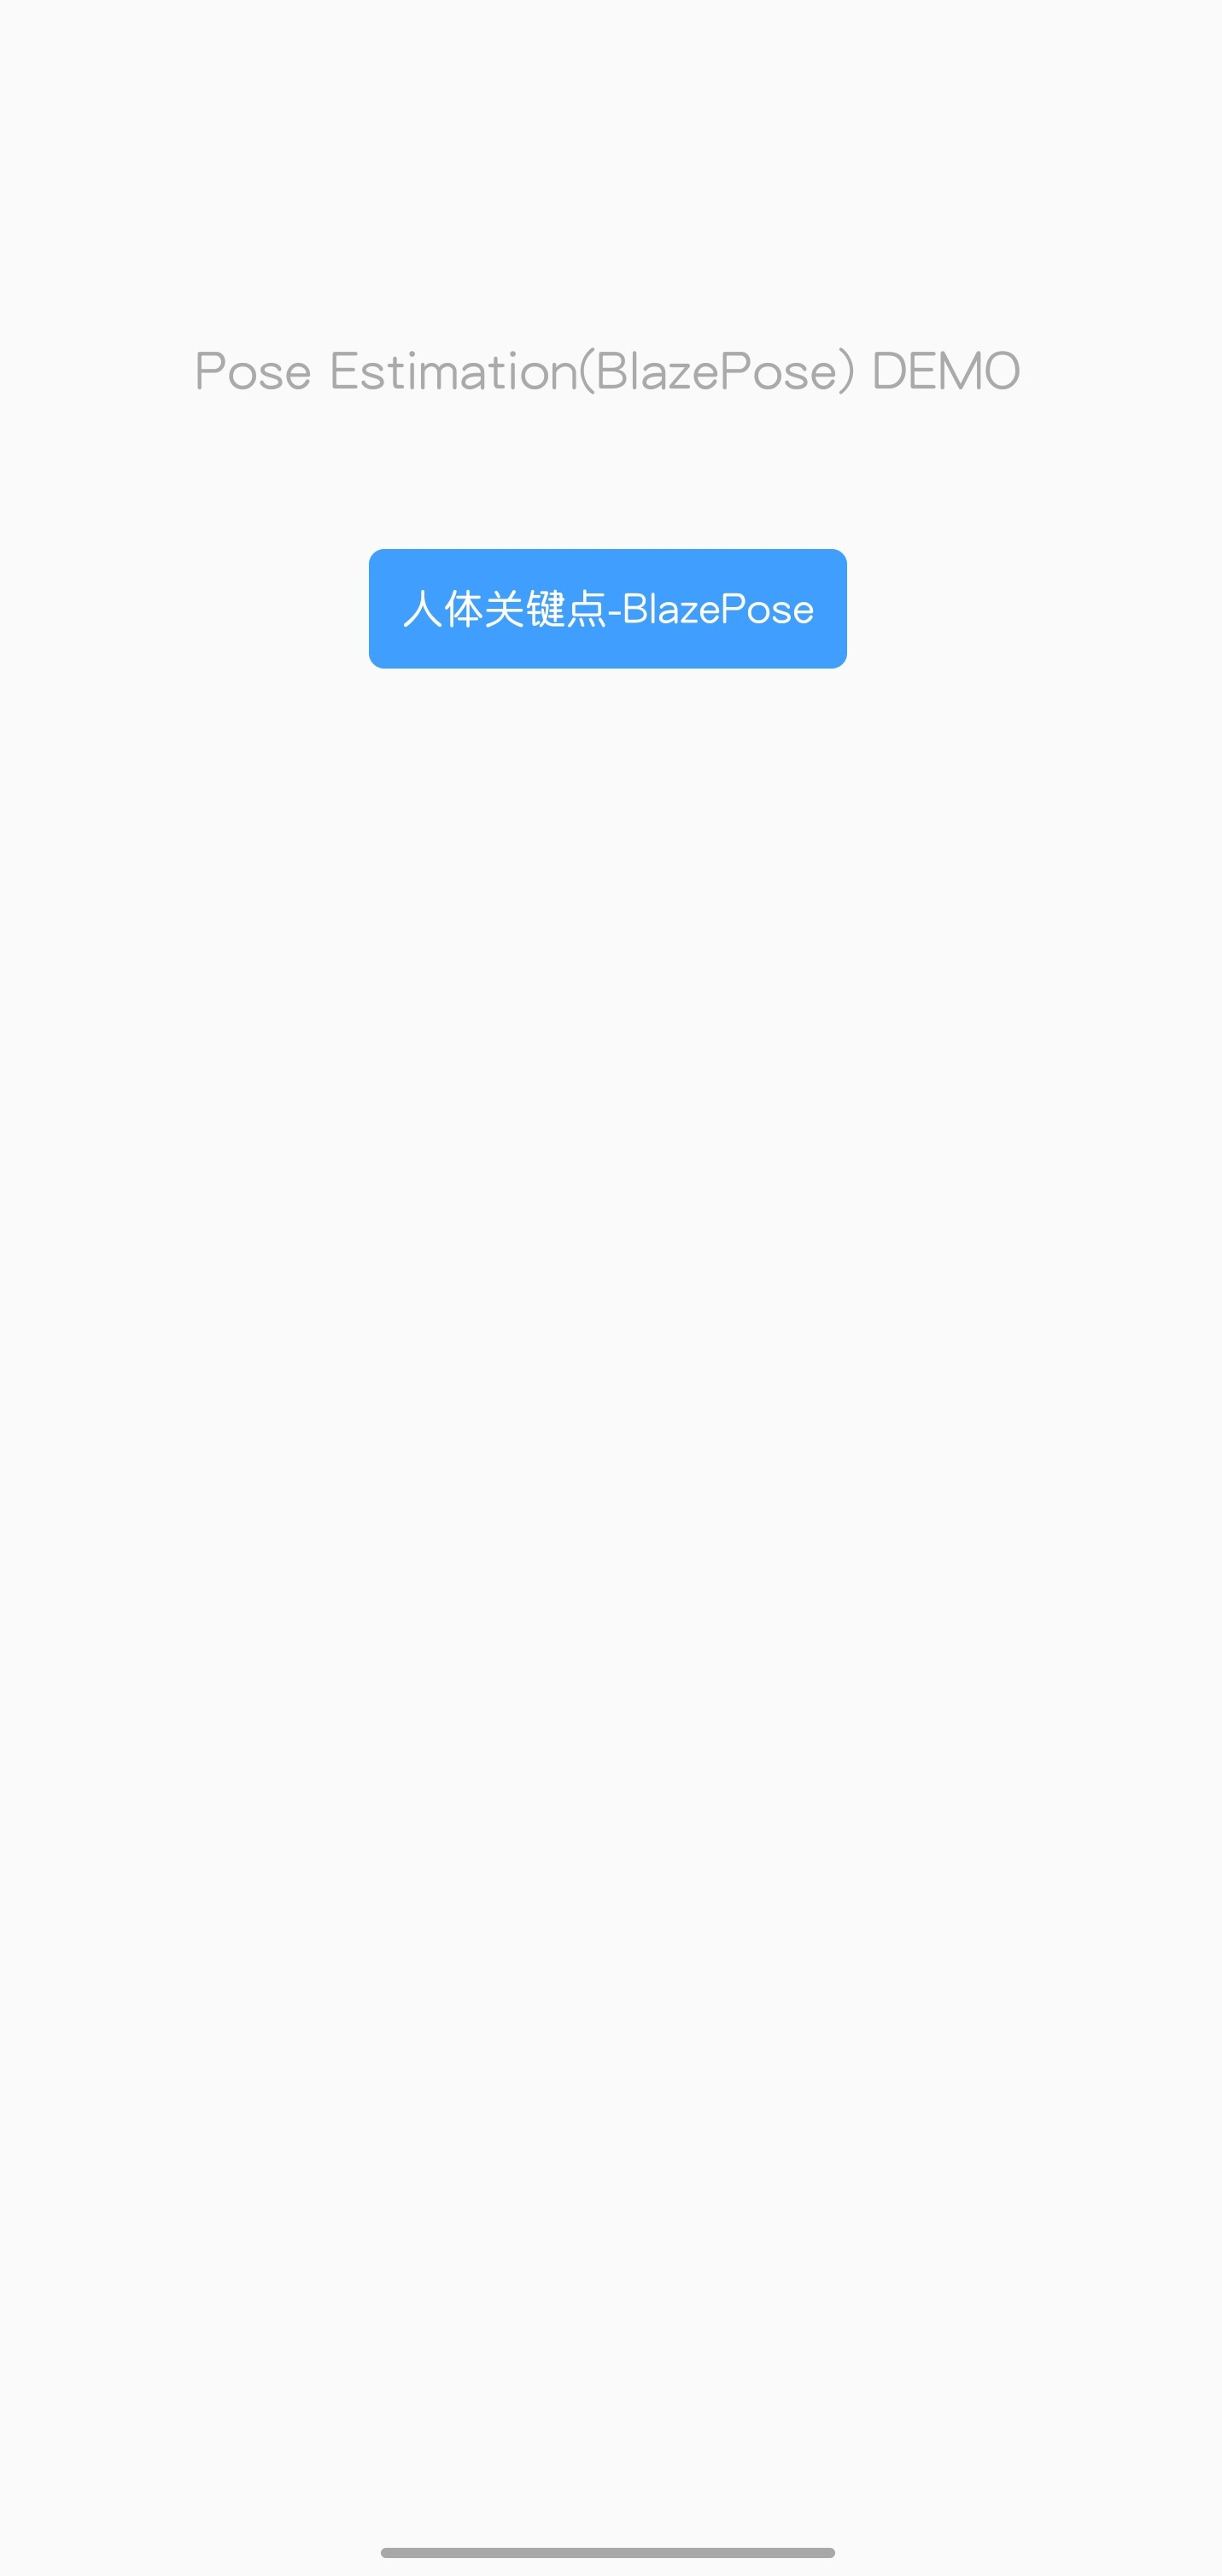
\includegraphics[width=0.18\textwidth]{mobile1}}
\hspace{2em}
\subfigure[arm上半身截图]{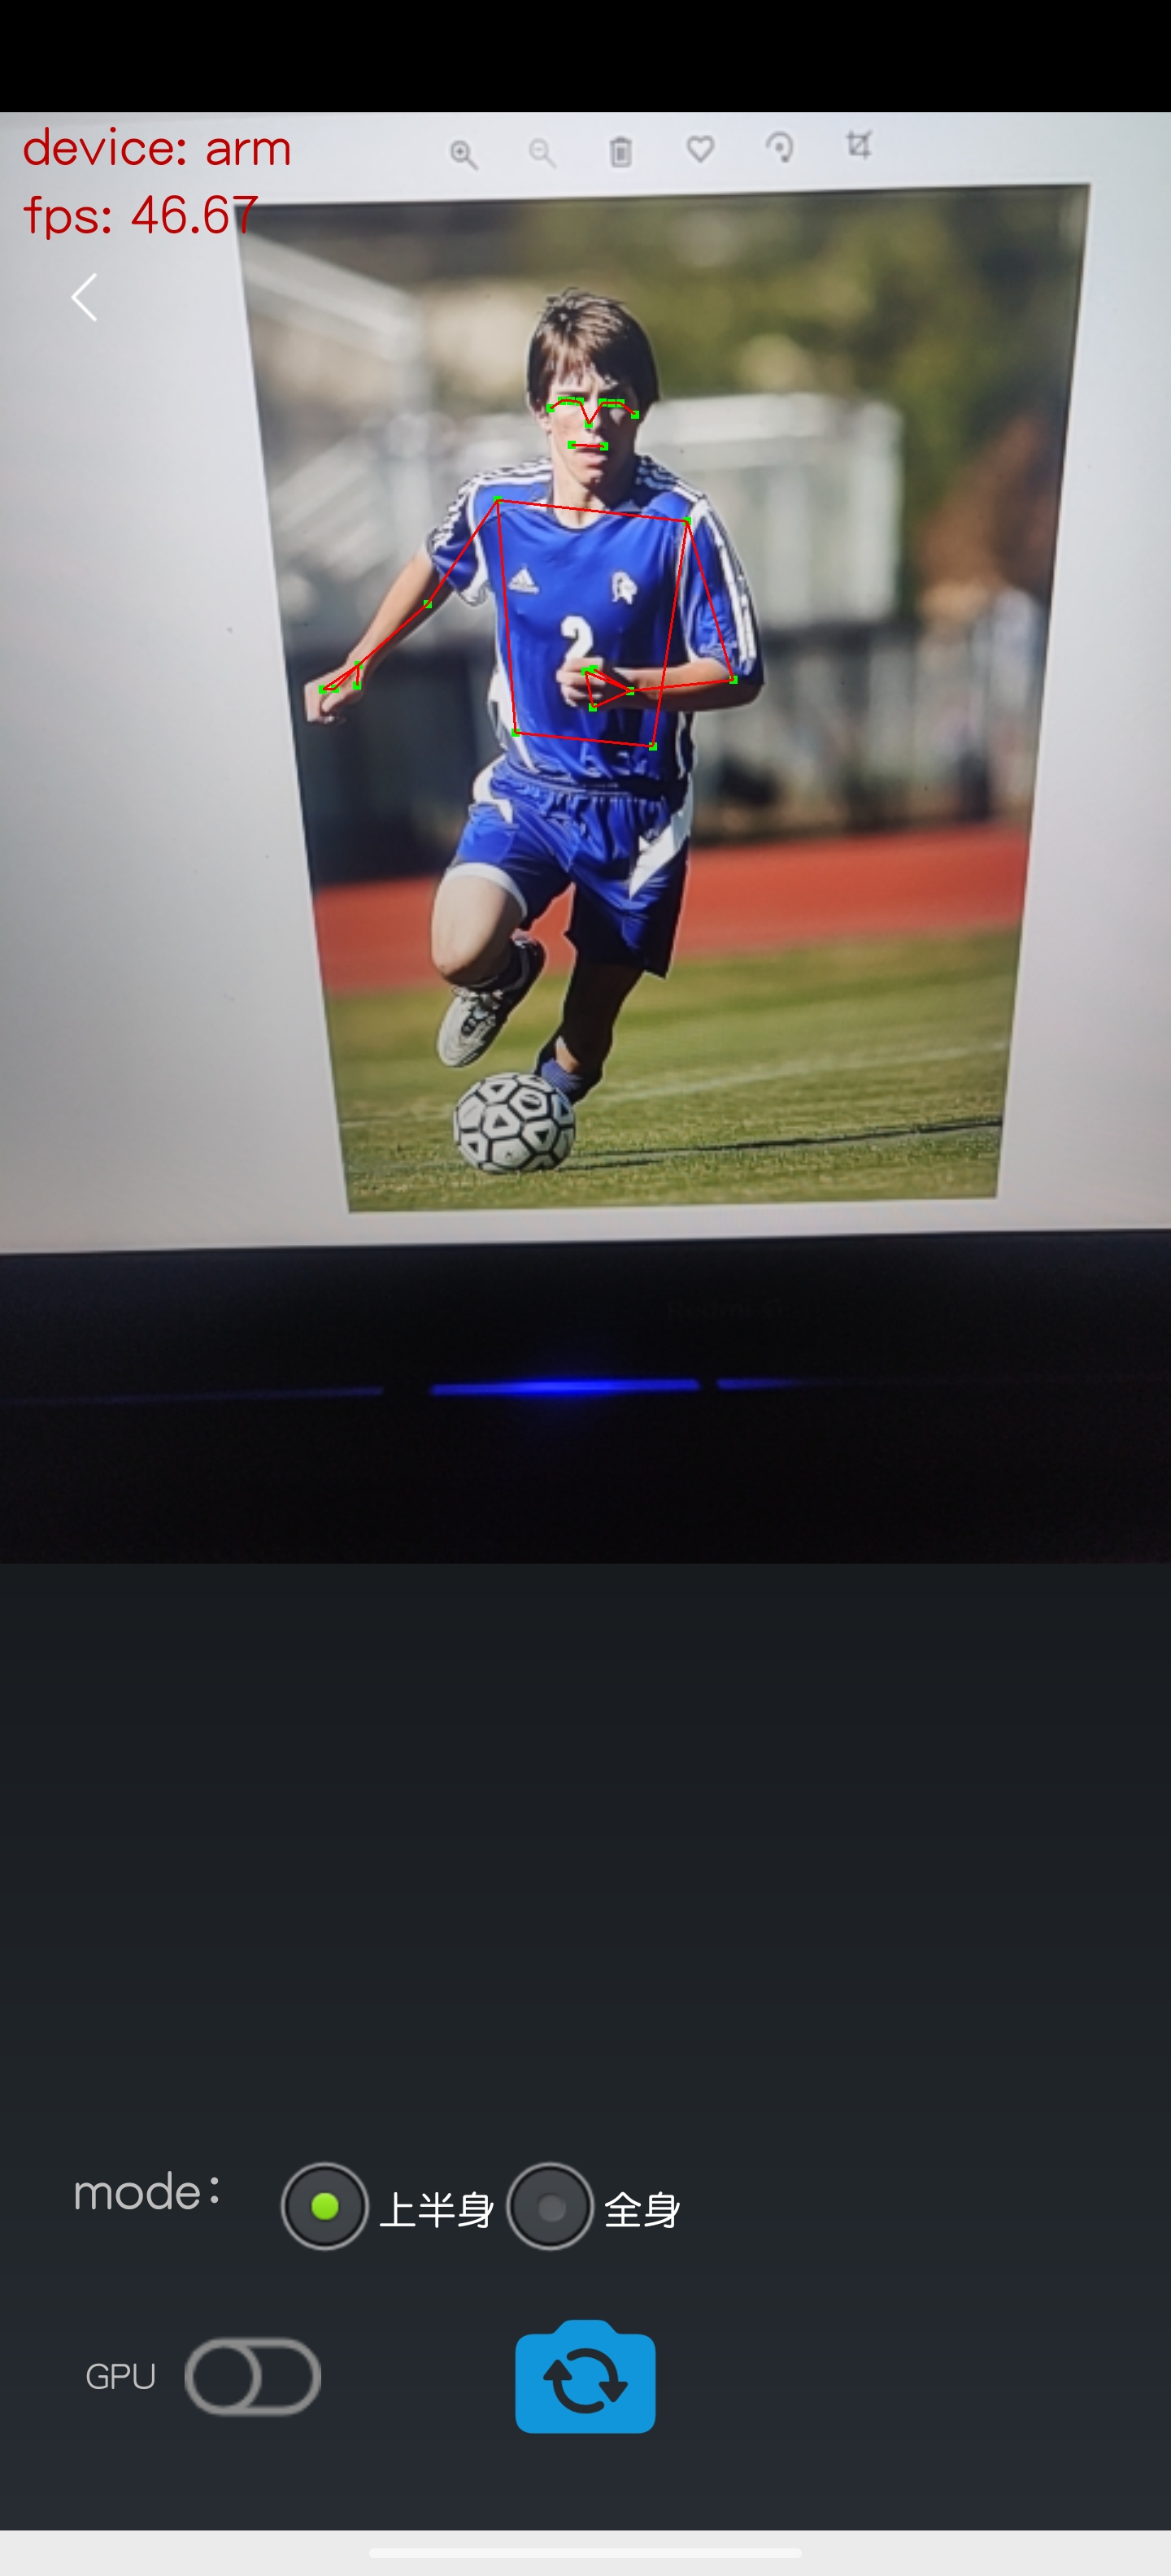
\includegraphics[width=0.18\textwidth]{mobile2}}
\hspace{2em}
\subfigure[arm全身截图]{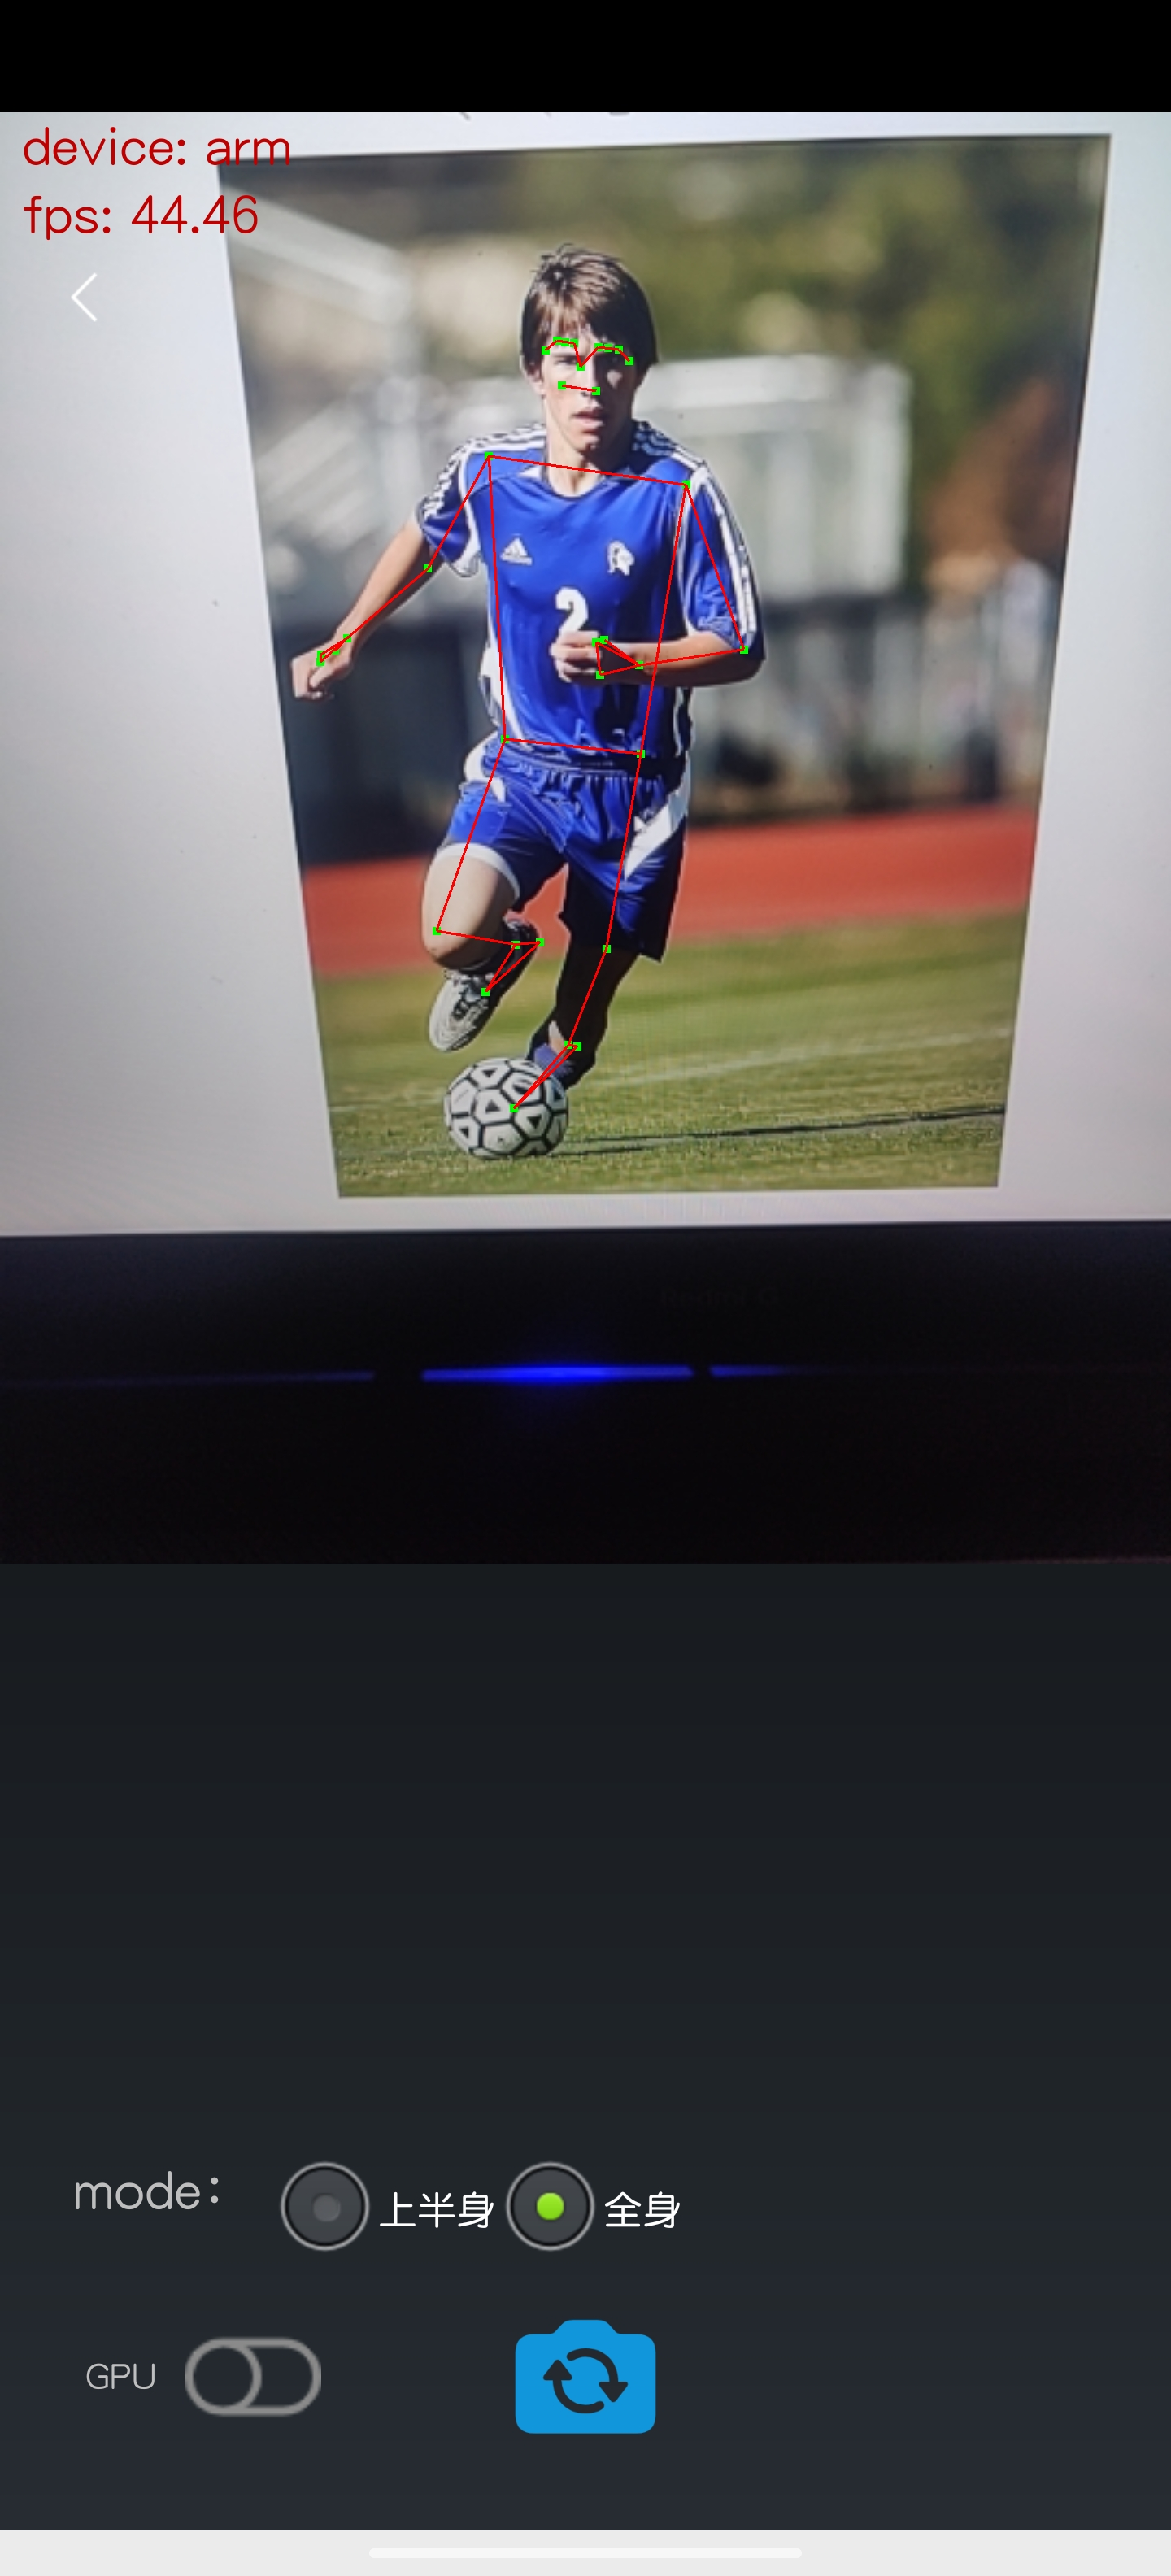
\includegraphics[width=0.18\textwidth]{mobile3}}
\end{minipage}
\centering
\begin{minipage}{\textwidth}
\centering
\subfigure[OpenCL上半身截图]{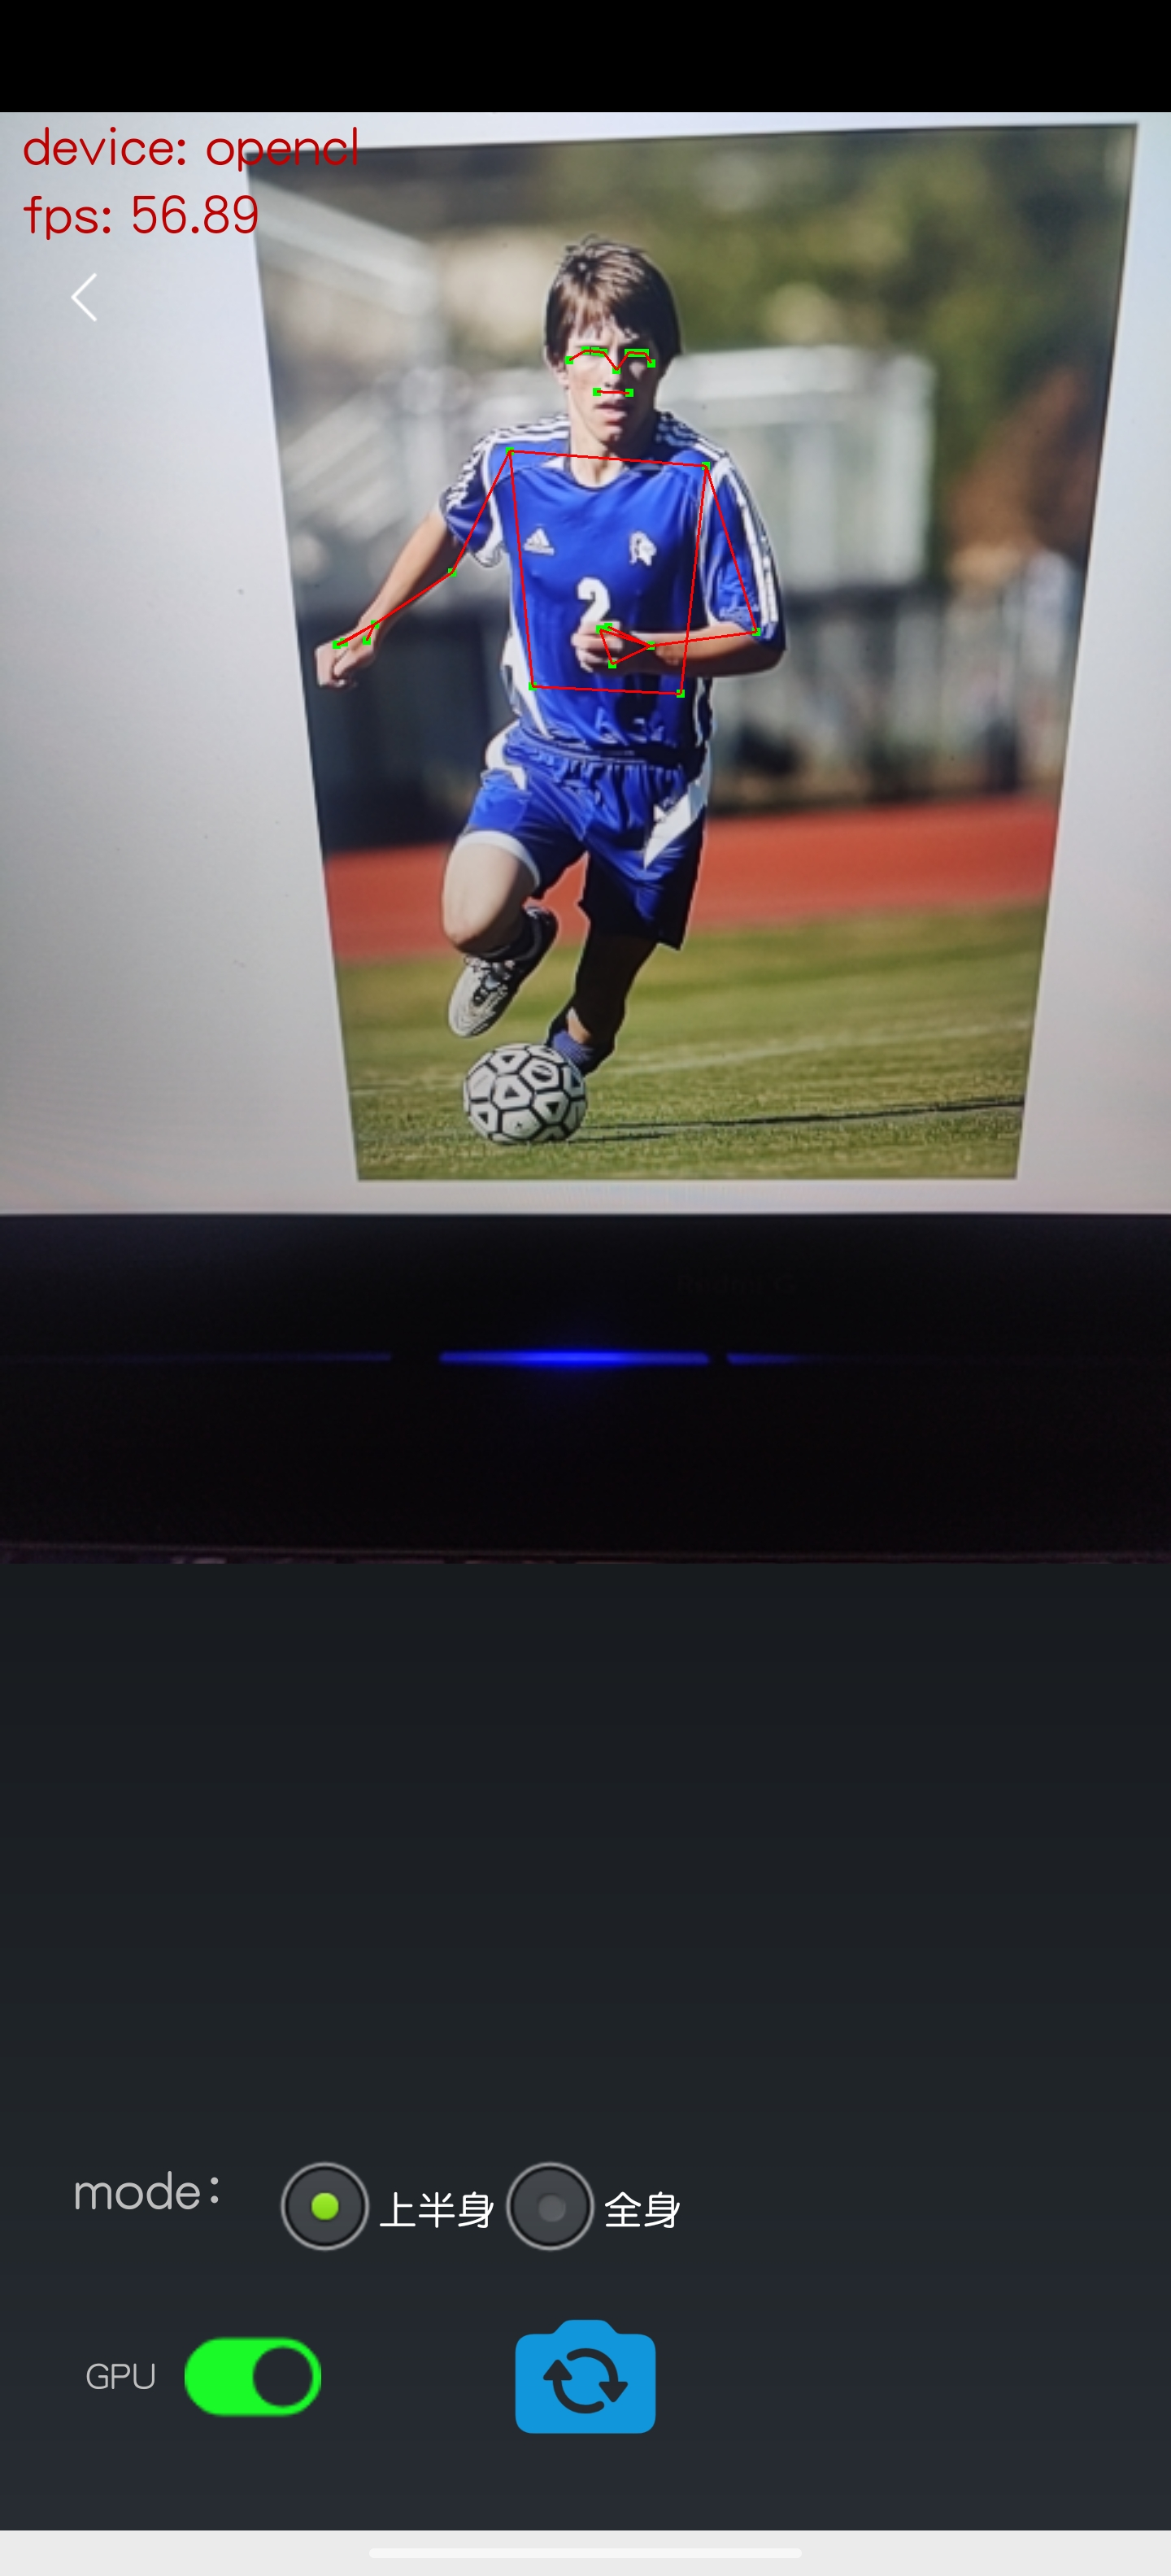
\includegraphics[width=0.18\textwidth]{mobile4}}
\hspace{2em}
\subfigure[OpenCL全身截图]{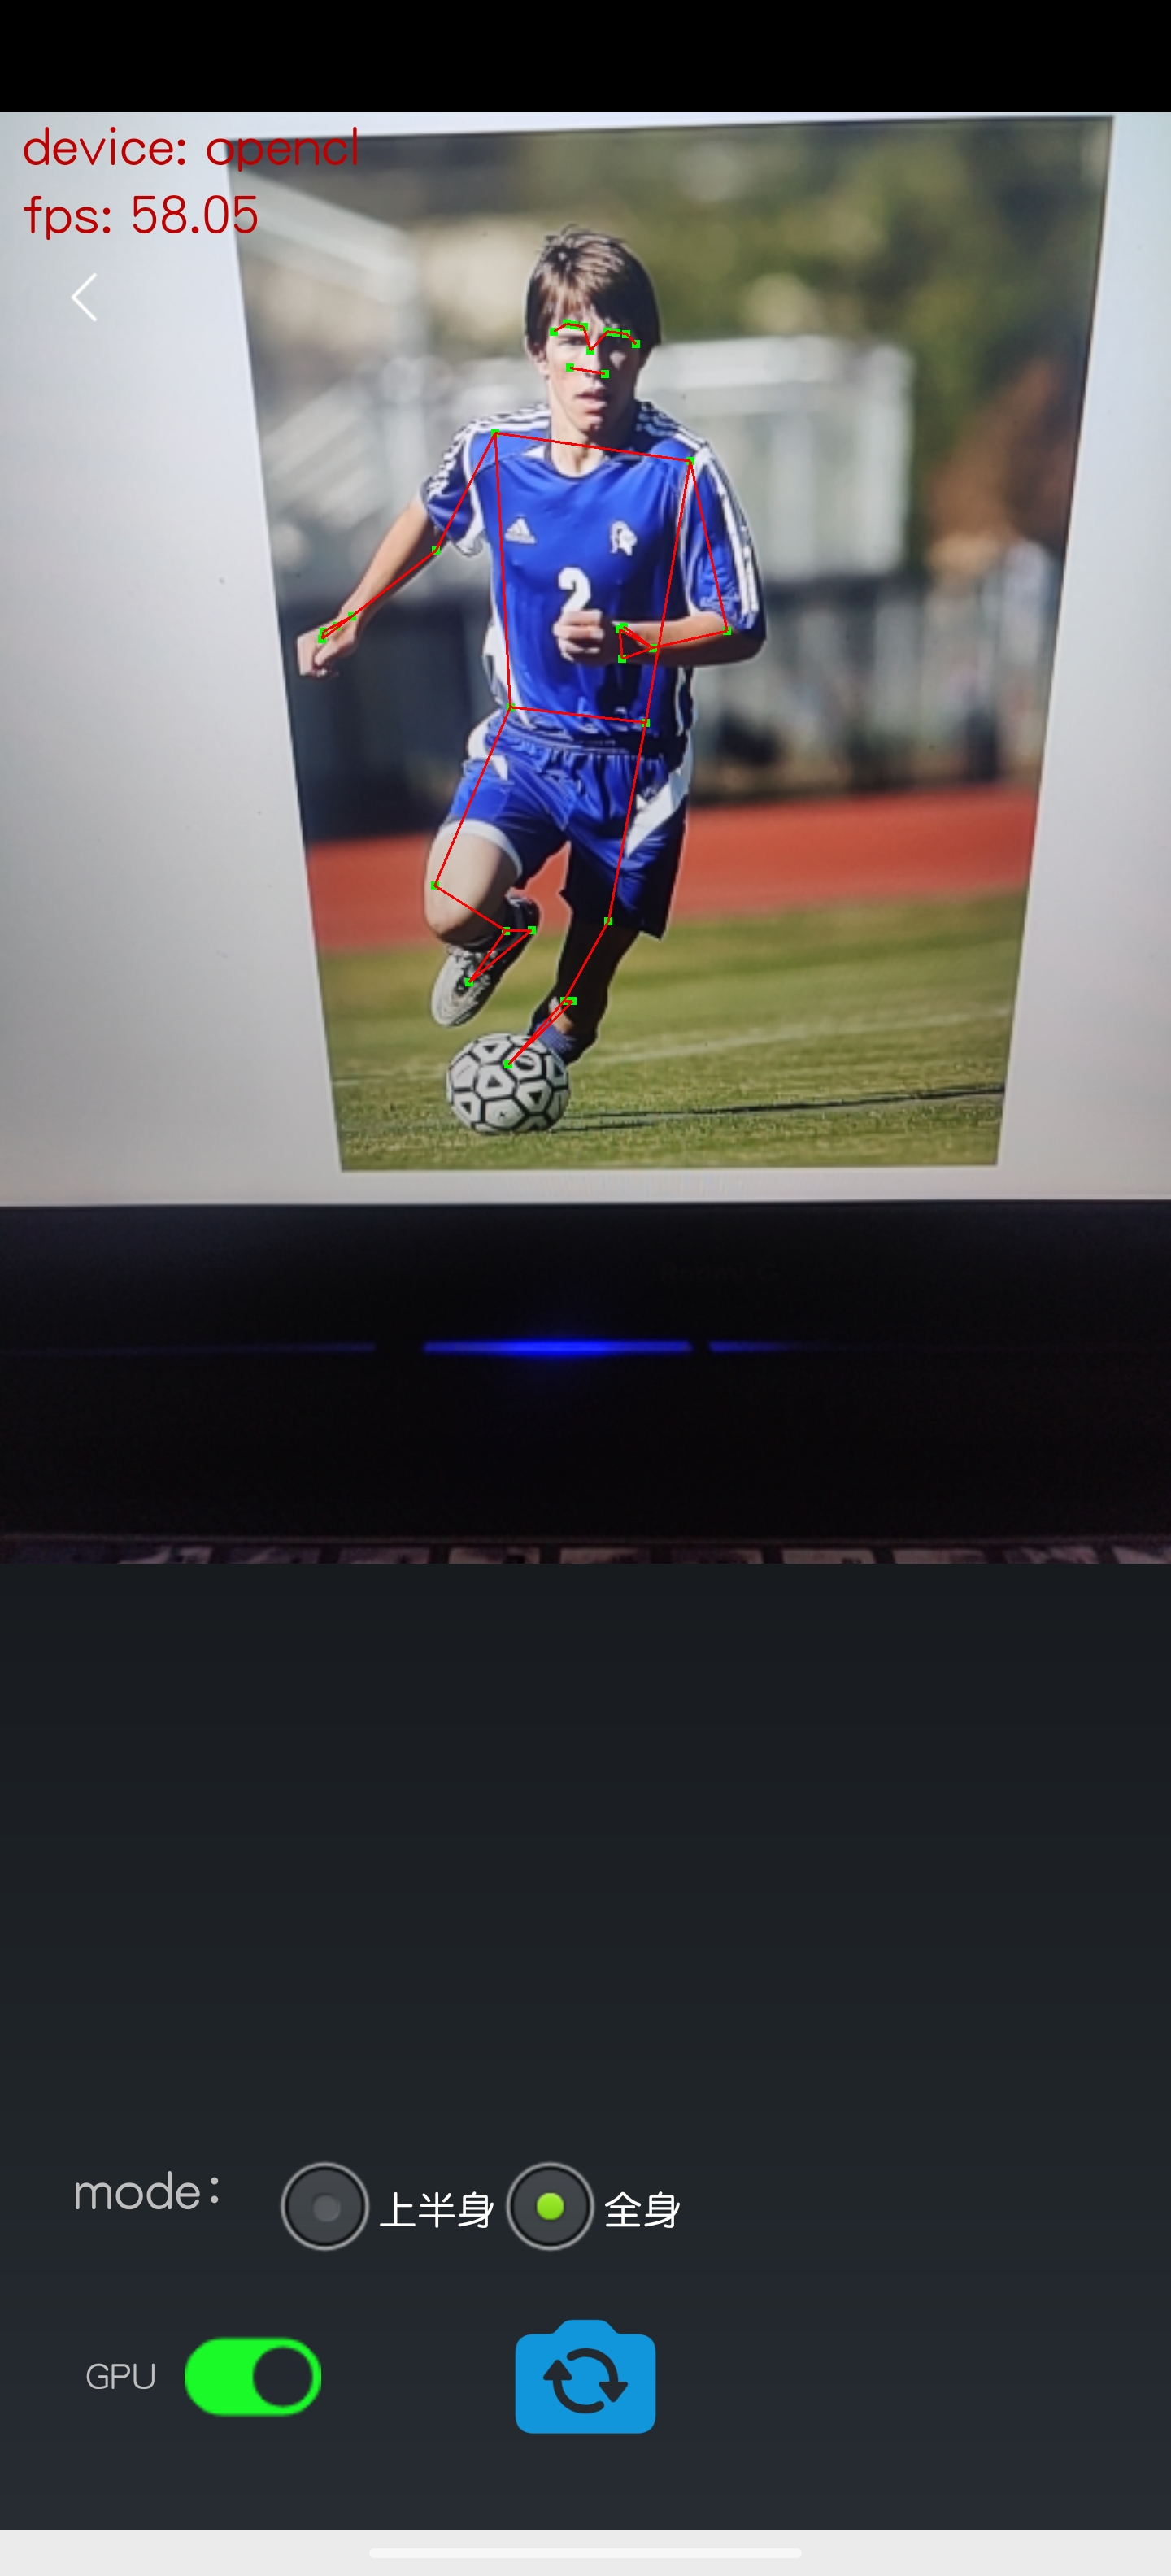
\includegraphics[width=0.18\textwidth]{mobile5}}
\end{minipage}
\vspace{0.2em}
\caption{移动端app截图}
\label{picture:23}
\end{figure}

\section{基于BlazePose的姿态模仿}

\subsection{虚拟机器人的姿态模仿}

本部分使用了unity3d创建了一个拥有33个关键点的虚拟火柴人。

再用python实时检测摄像头或者视频输入。获得每个点的相对位置和角度角度。使用UDP,创建了在本机``127.0.0.1''上的5052端口,在此端口上进行数据传输,将每个点的位置传输到unity中,从而使得机器人能够姿态模仿。

对于unity3d的虚拟火柴人进行姿态模仿结果如图~\ref{picture:24}~所示。

\begin{figure}[!h]
\setlength{\subfigcapskip}{-1bp}
\centering
\begin{minipage}{\textwidth}
\centering
\subfigure{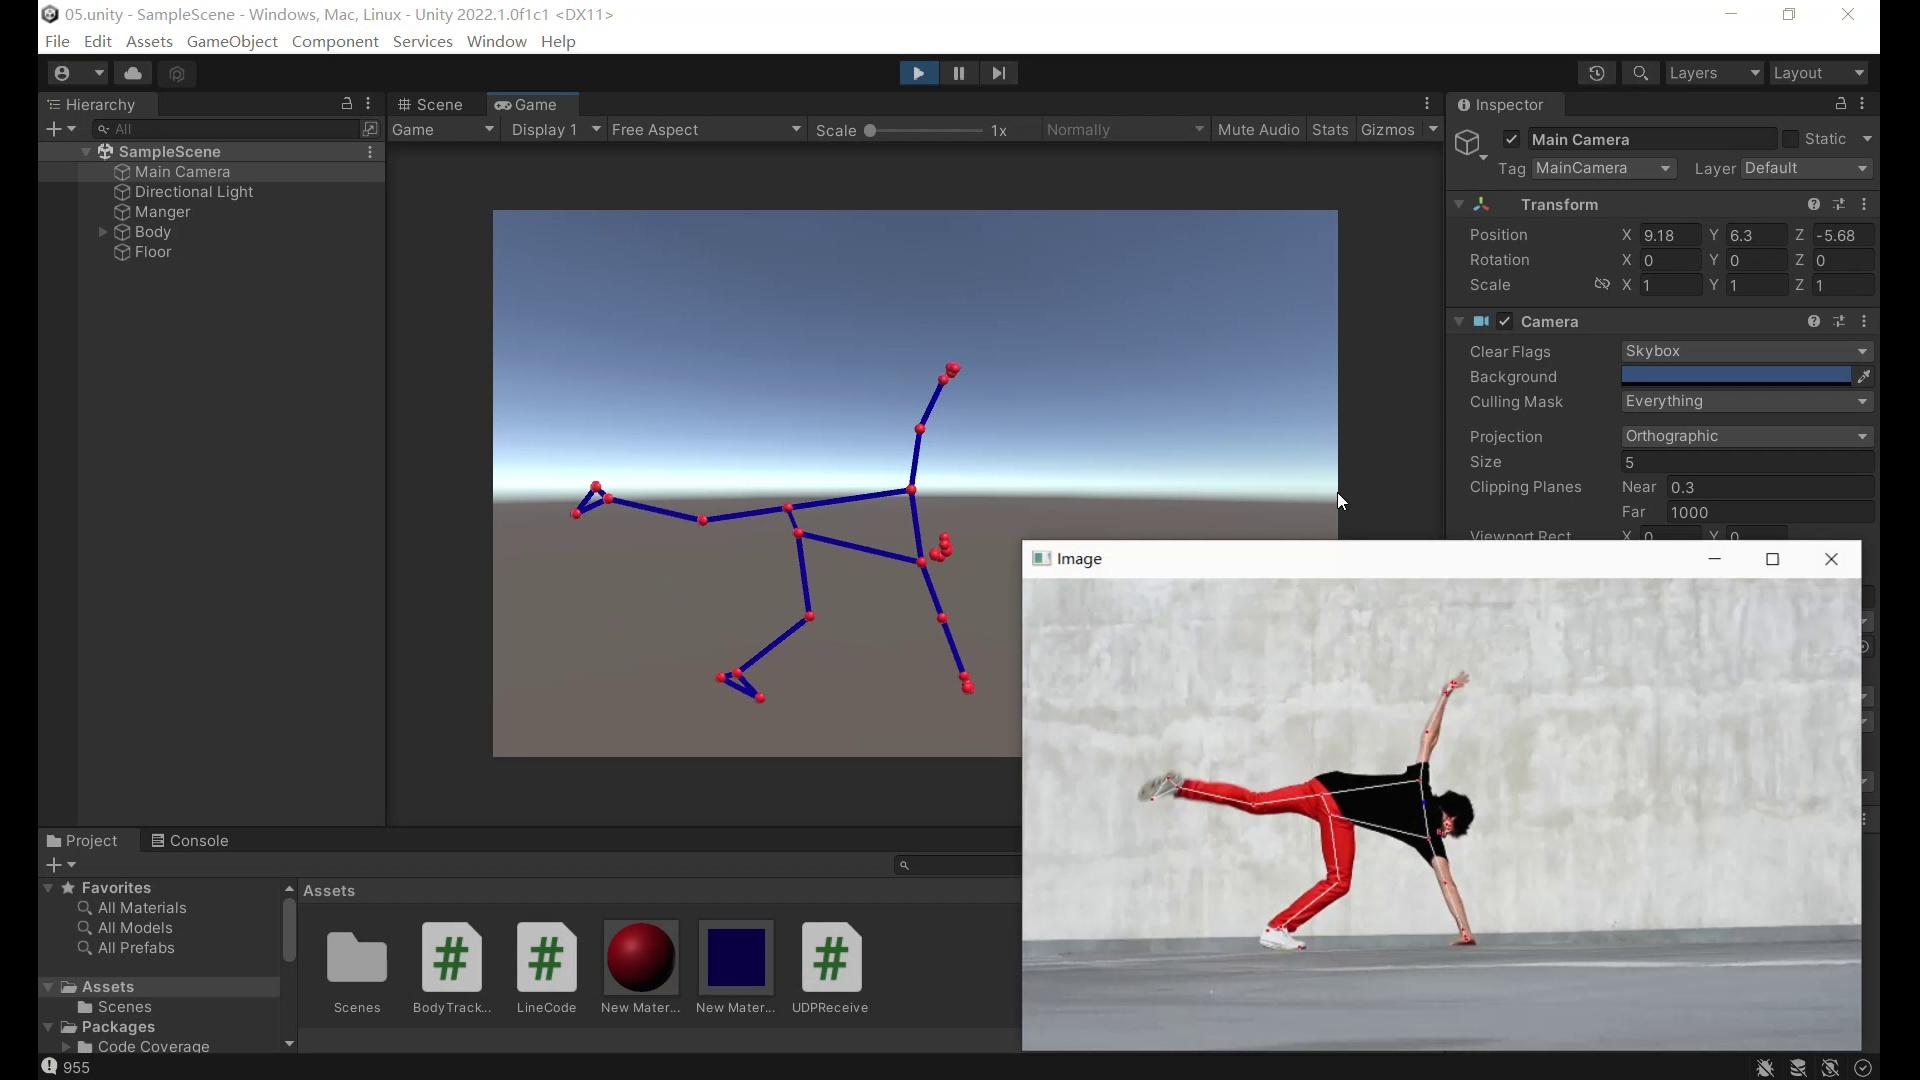
\includegraphics[width=0.24\textwidth]{unity1}}
\subfigure{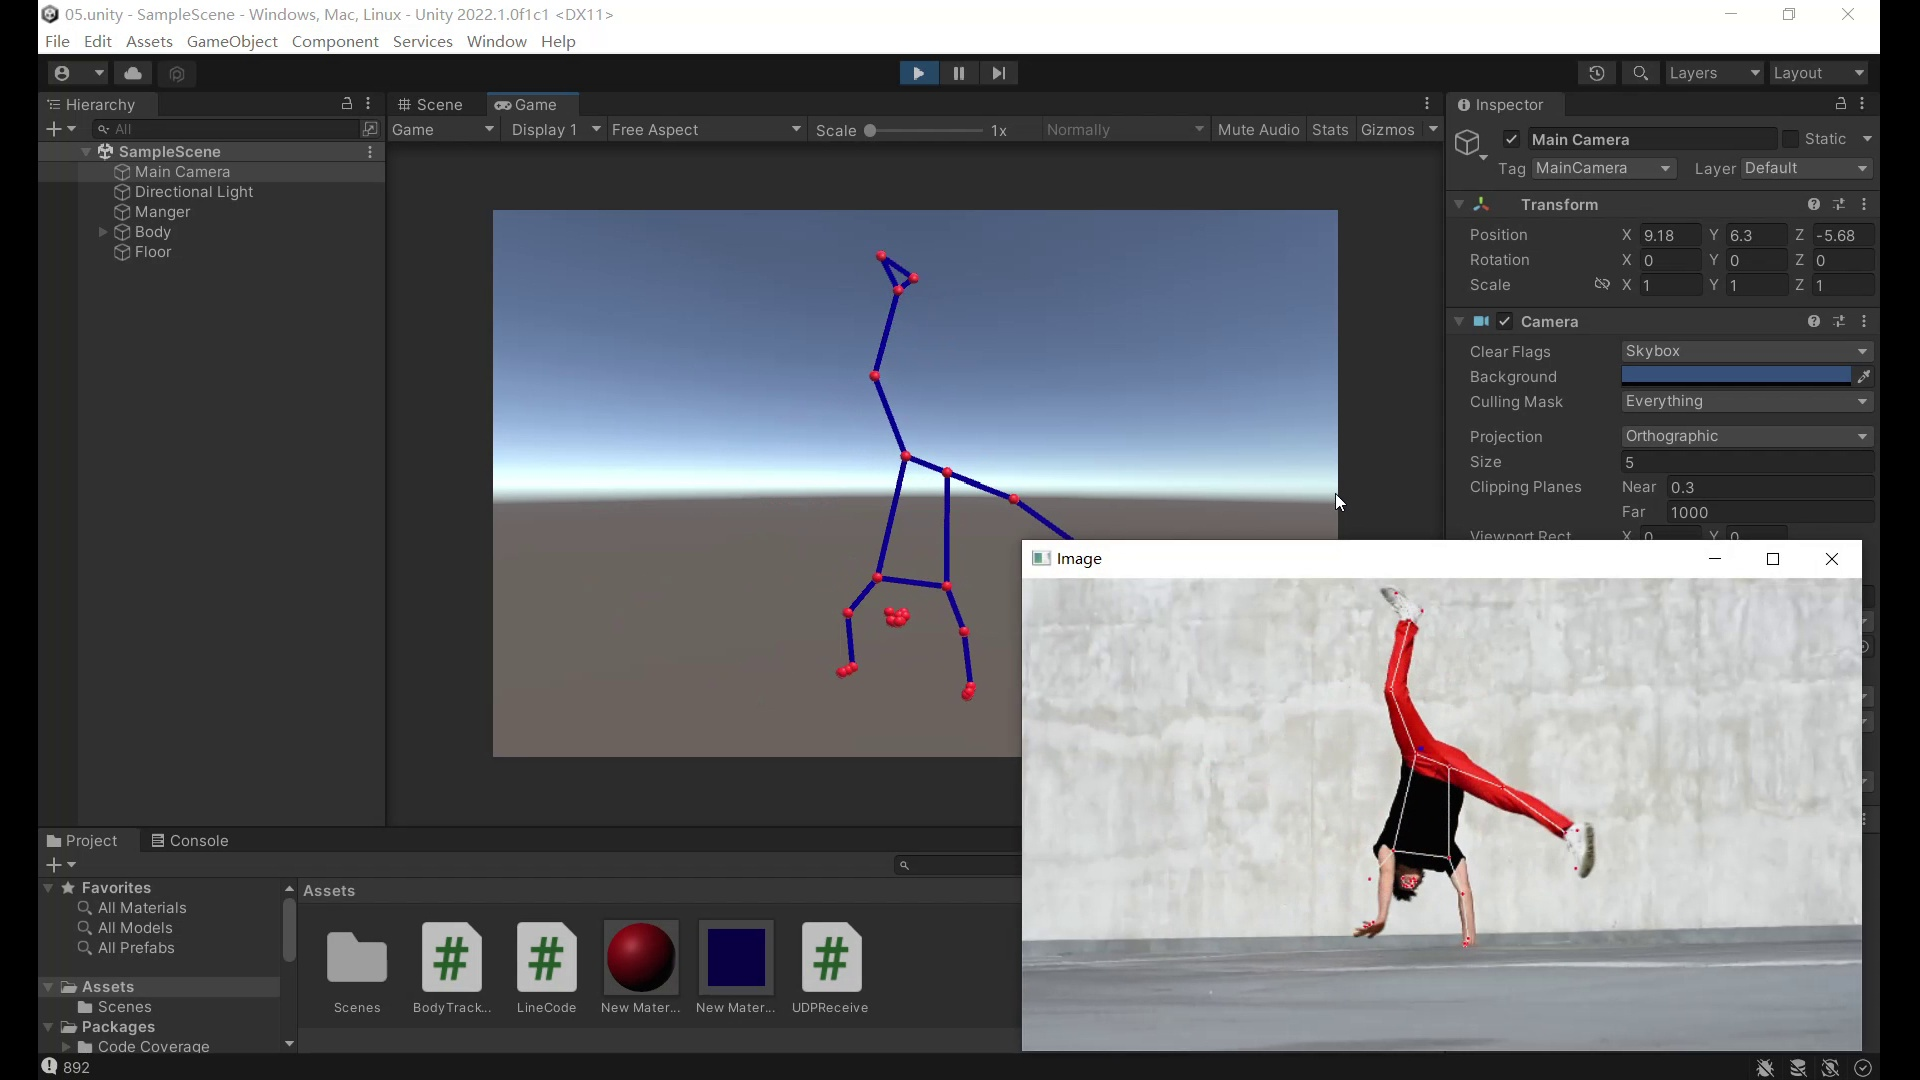
\includegraphics[width=0.24\textwidth]{unity2}}
\subfigure{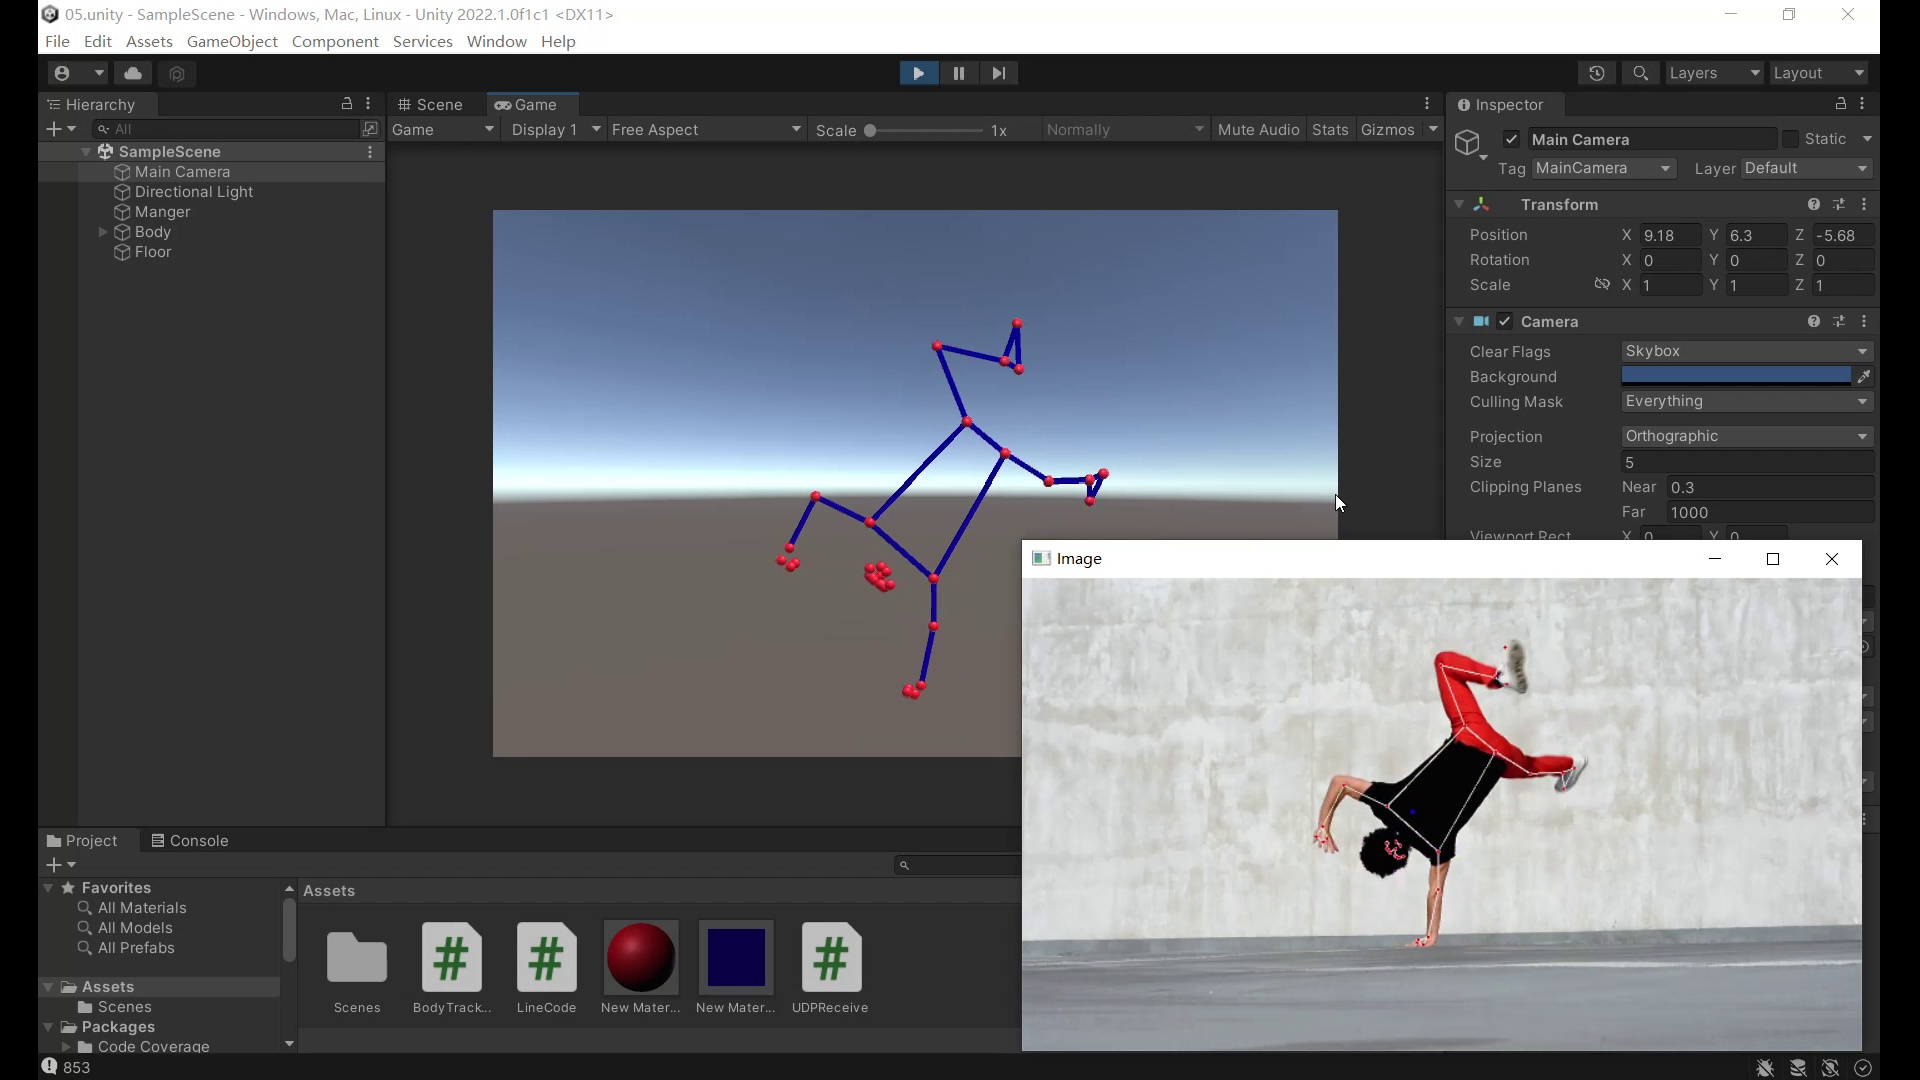
\includegraphics[width=0.24\textwidth]{unity3}}
\subfigure{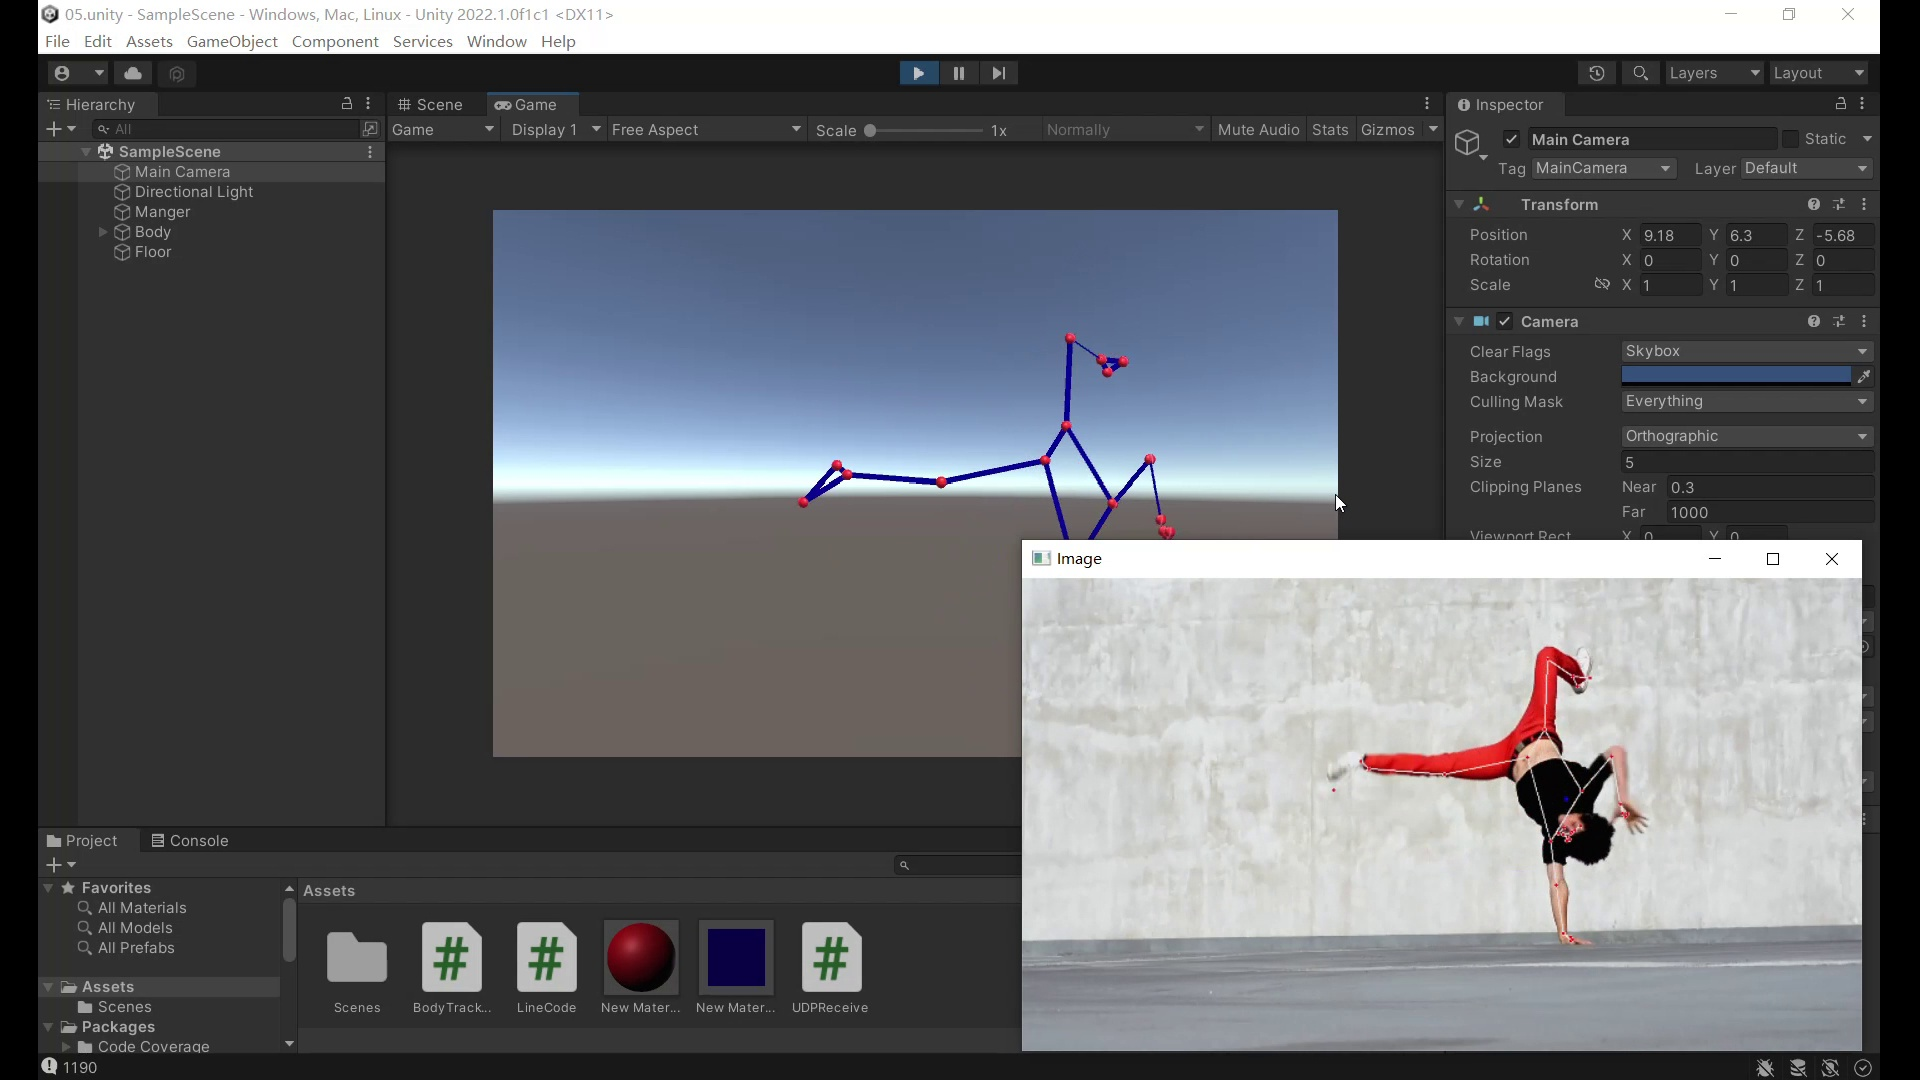
\includegraphics[width=0.24\textwidth]{unity4}}
\end{minipage}
\begin{minipage}{\textwidth}
\centering
\subfigure{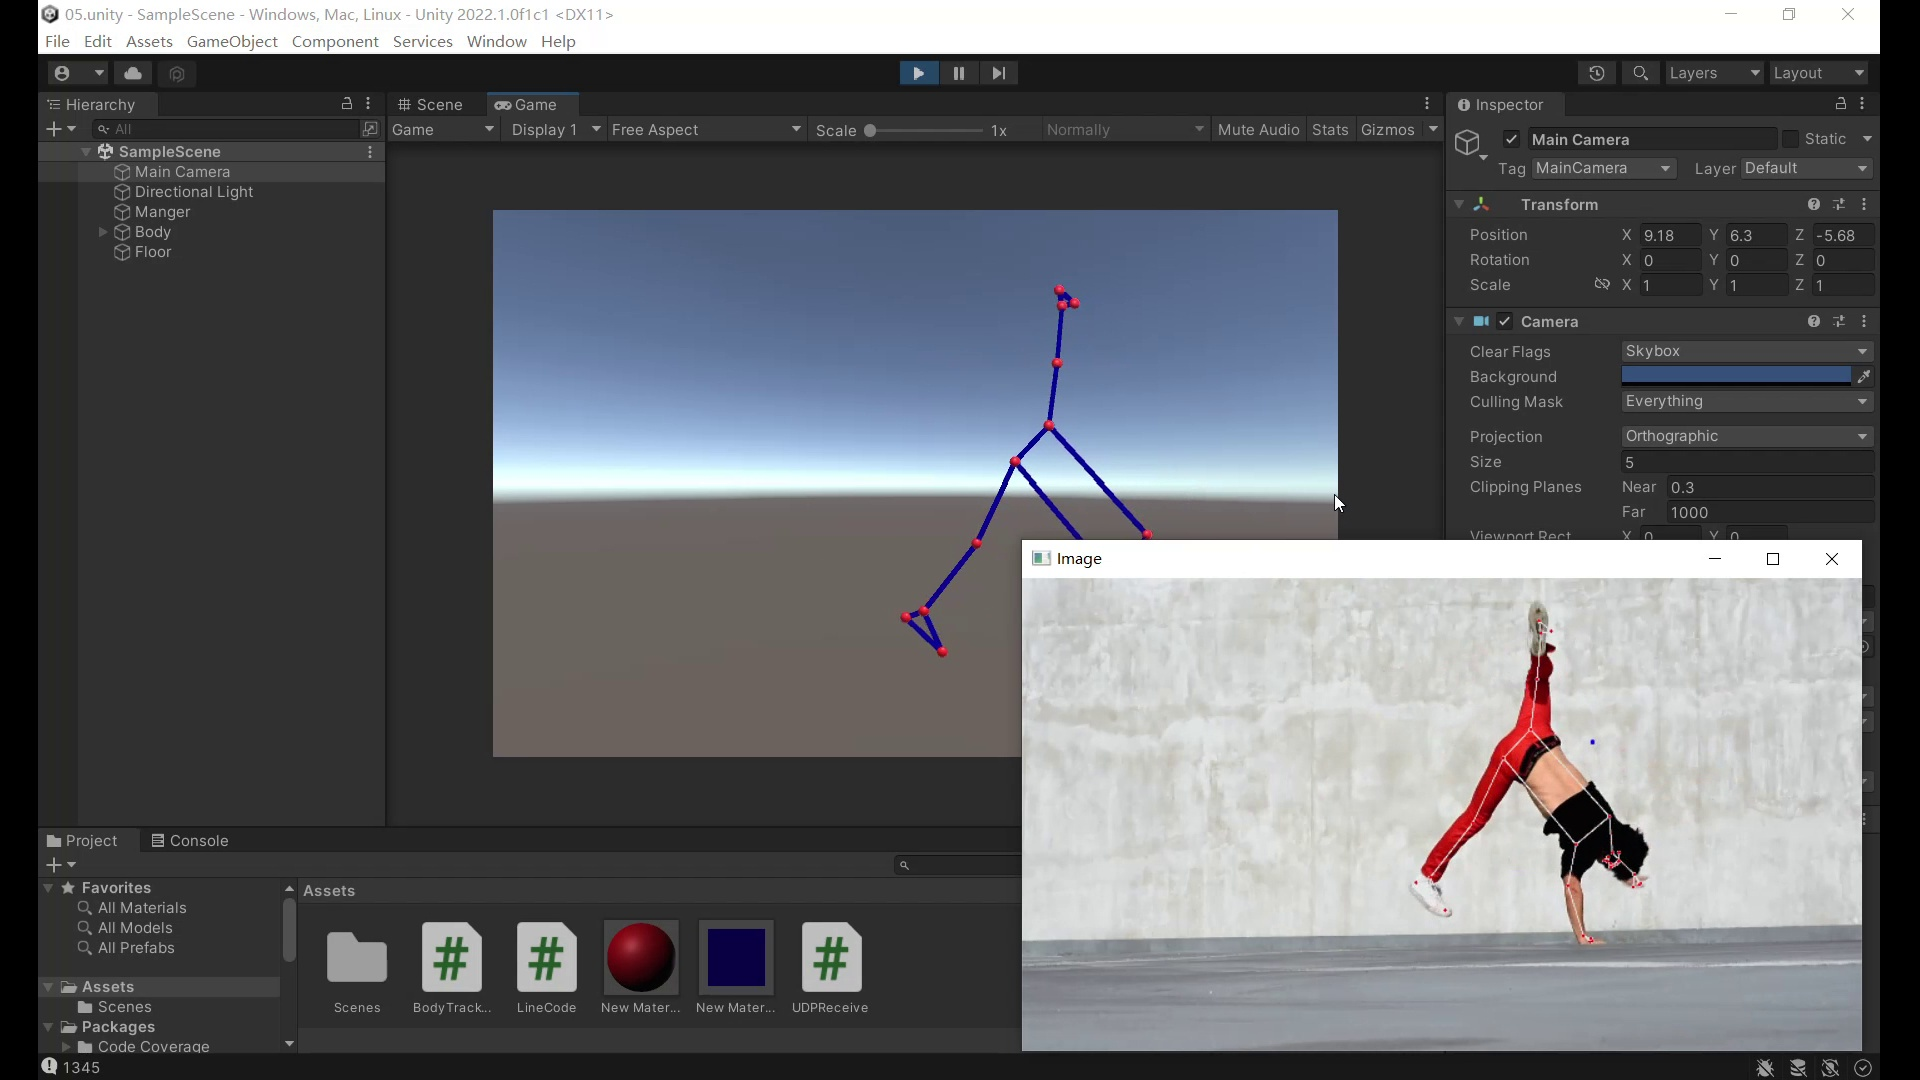
\includegraphics[width=0.24\textwidth]{unity5}}
\subfigure{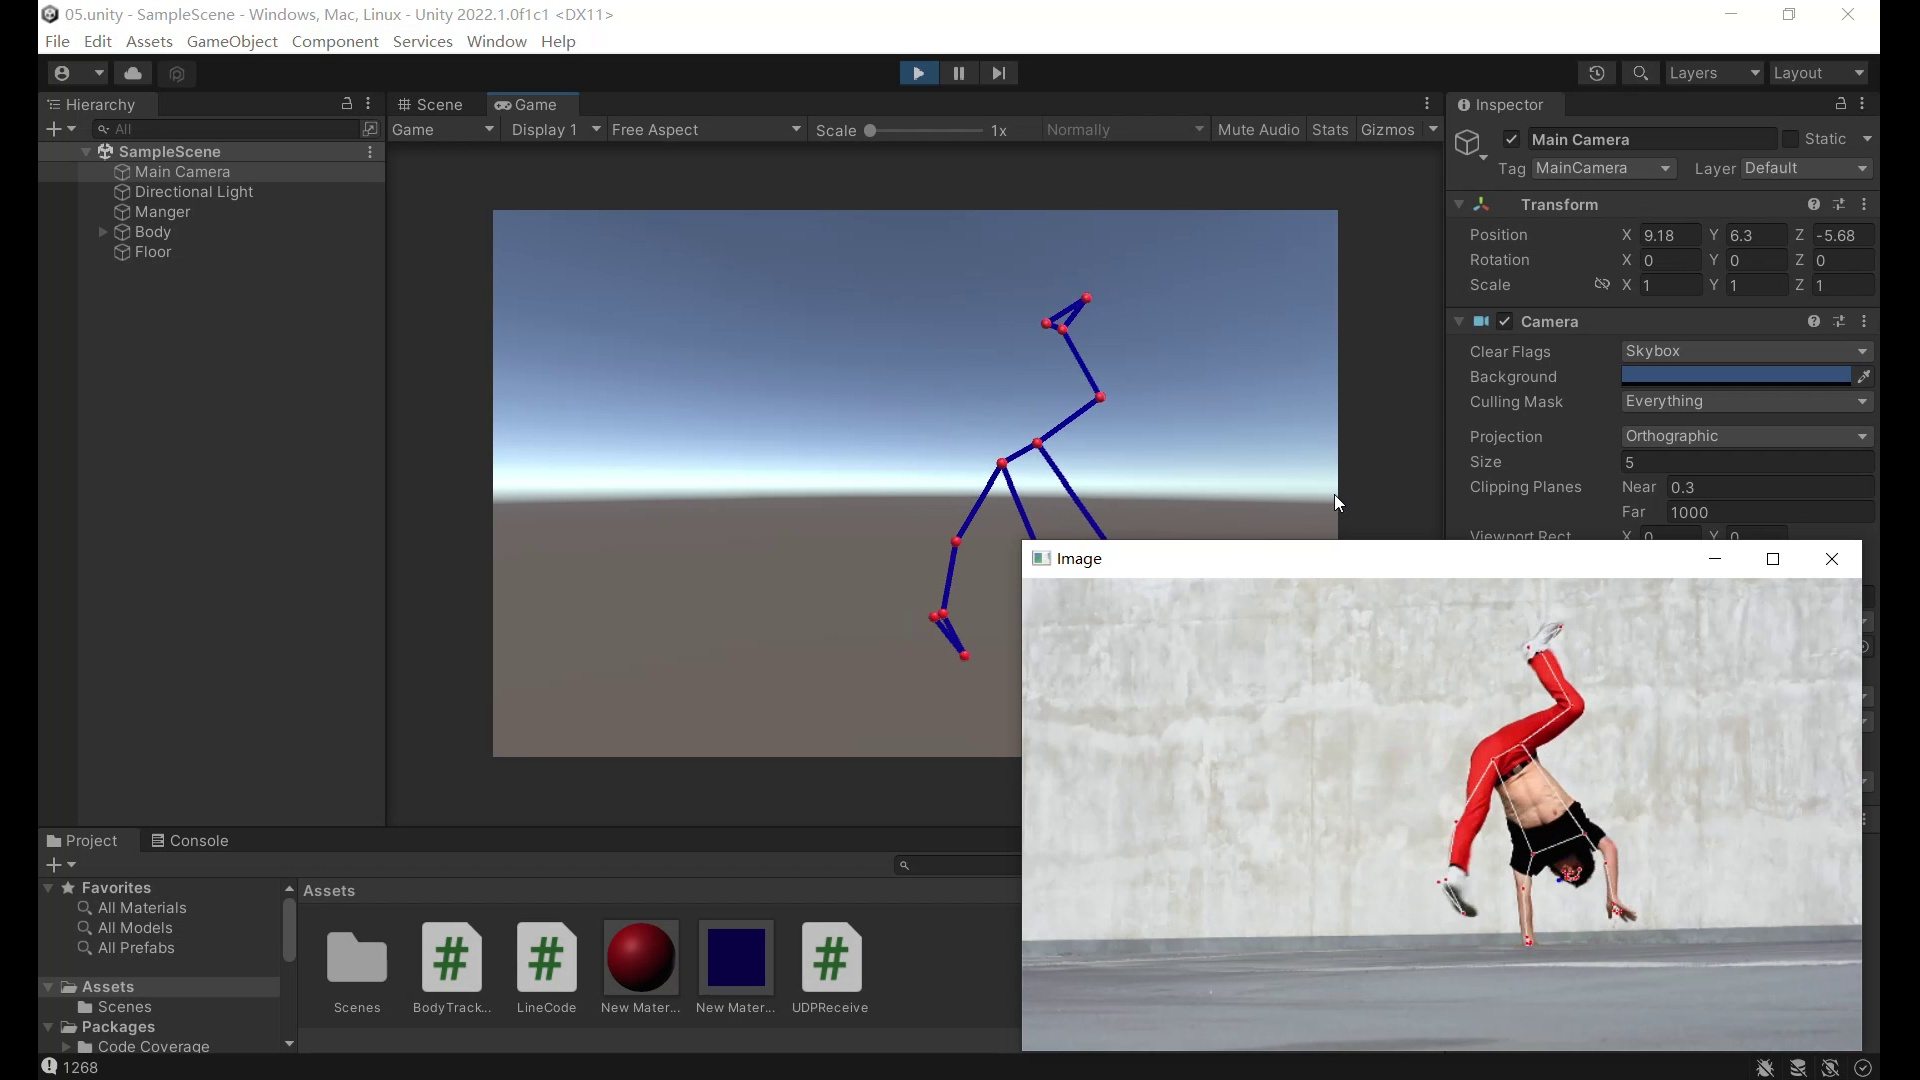
\includegraphics[width=0.24\textwidth]{unity6}}
\subfigure{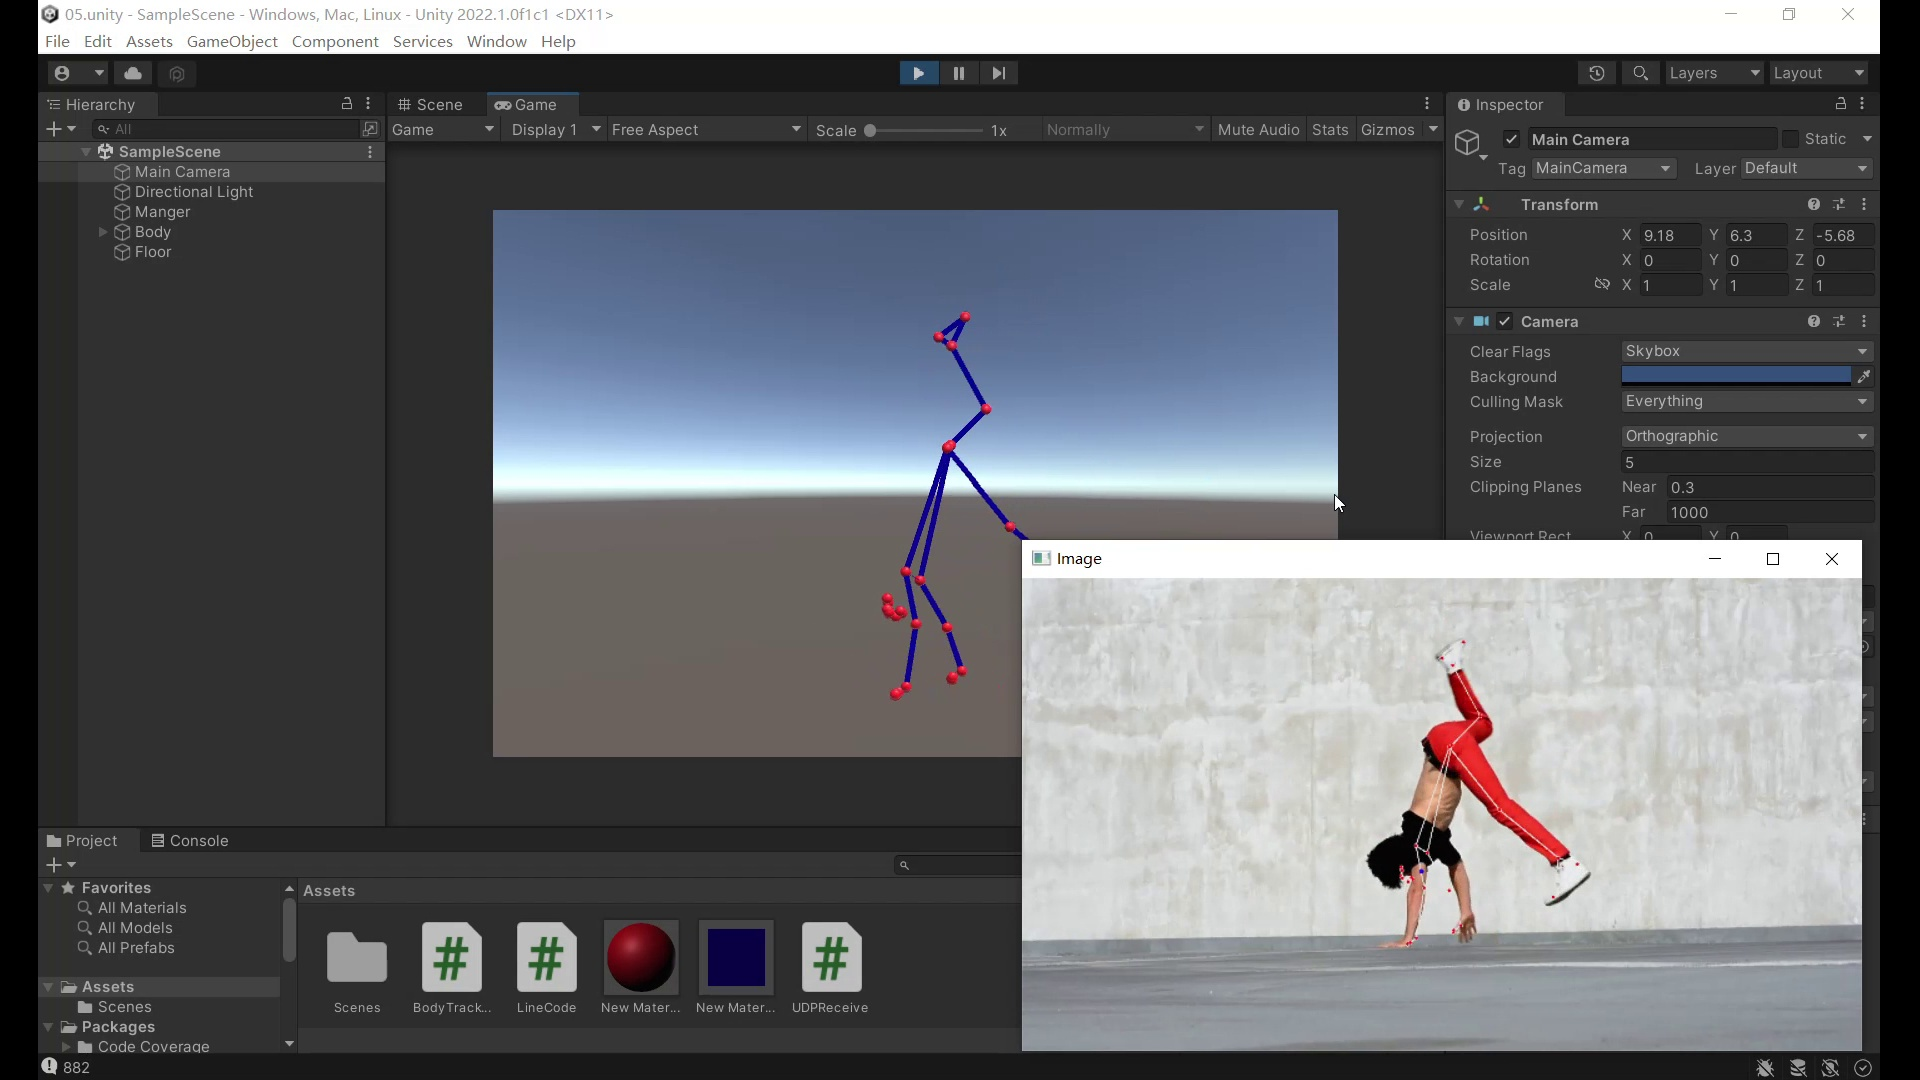
\includegraphics[width=0.24\textwidth]{unity7}}
\subfigure{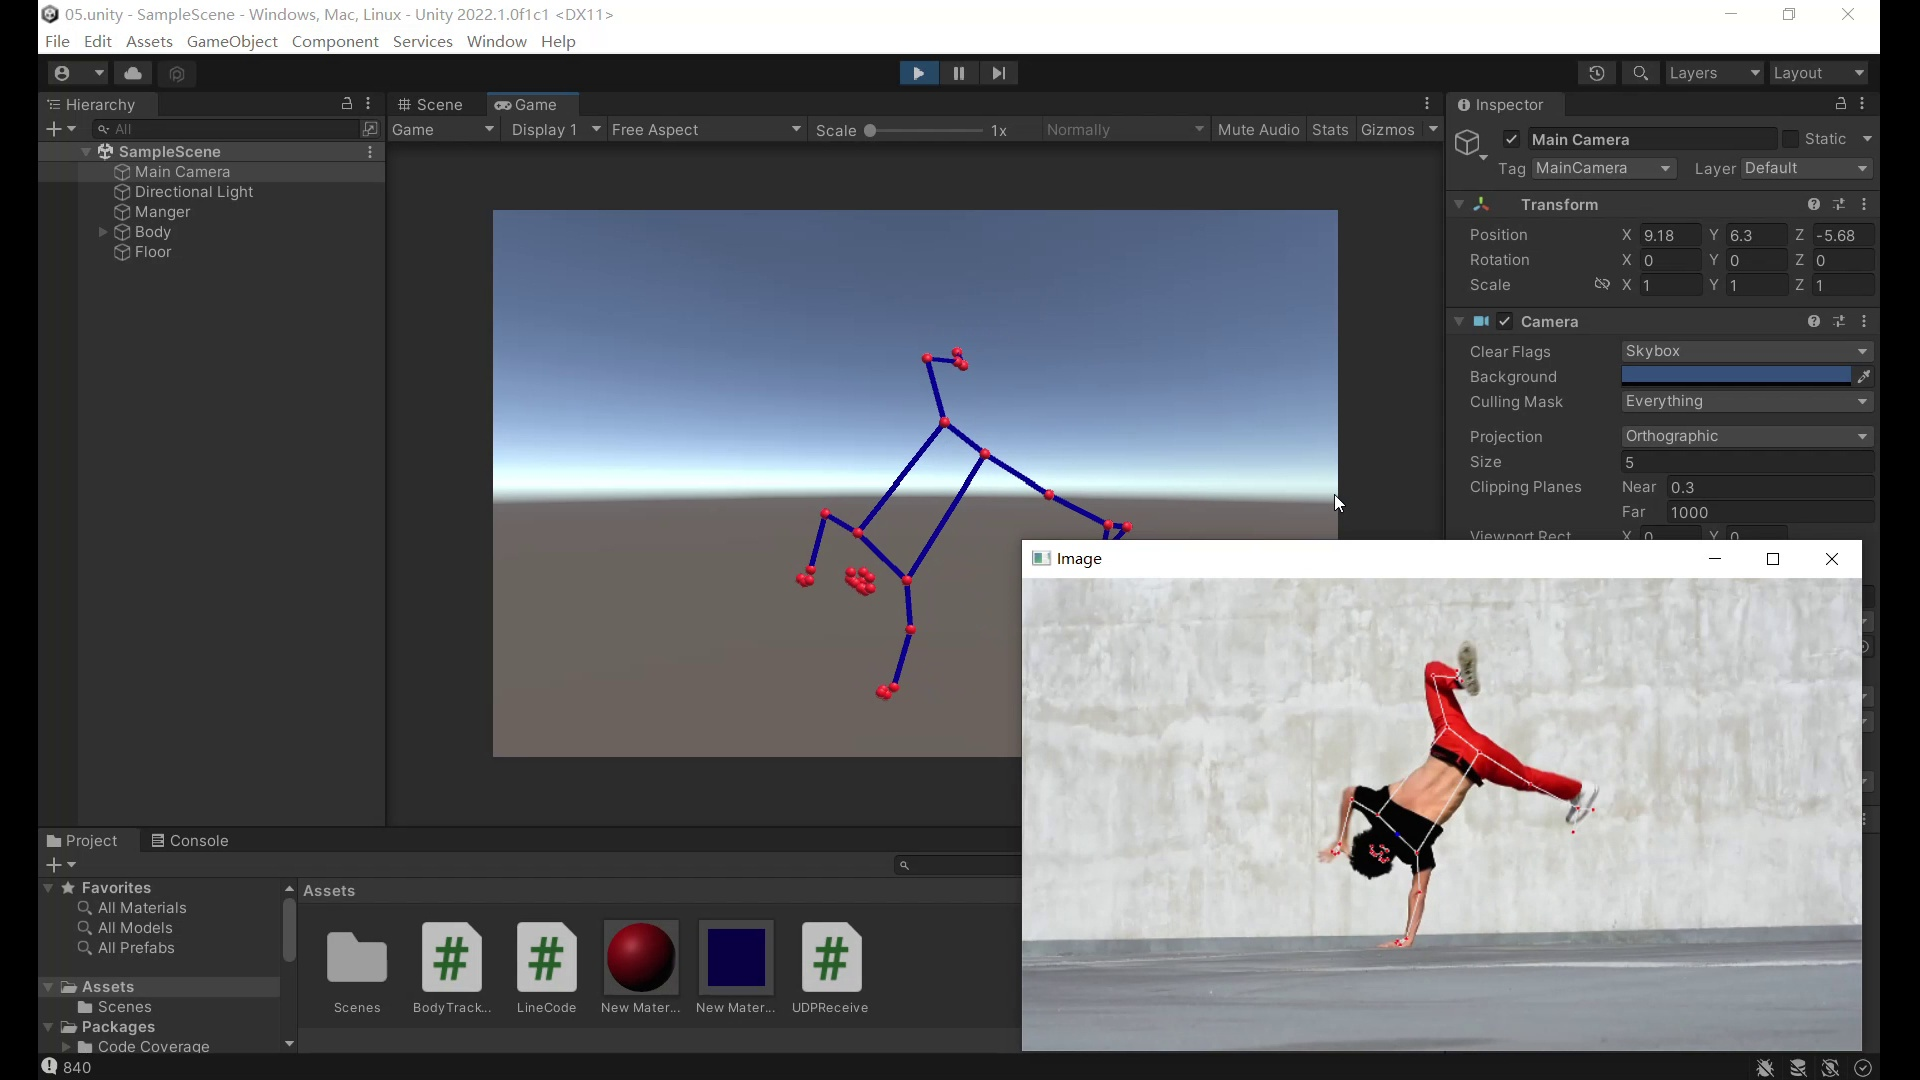
\includegraphics[width=0.24\textwidth]{unity8}}
\end{minipage}
\vspace{0.2em}
\caption{unity虚拟火柴人姿态模仿截图}
\label{picture:24}
\end{figure}

\subsection{真实机器人的姿态模仿}

对于真实机器人,我们使用arduino开发板和SG90舵机来完成实验,arduino开发板指导SG90舵机调整旋转角度,从而达到完成姿态模仿的效果。至于数据传输,我们使用USB串联,主要库为serial。

以右肘部姿态模仿为例,如图~\ref{piture:16}~所示,我们只需计算12-14-16的夹角即可。

记关键点12为$P_1$,关键点14为$P_2$,关键点16为$P_3$,如图~\ref{picture:25}~所示,我们使用math.atan2函数,分别计算出线$P_3P_2$和$X$轴的夹角$\angle P_3P_2X$和线$P_1P_2$和$X$轴的夹角$\angle P_1P_2X$,然后再用$\angle P_3P_2X-\angle P_1P_2X$即可得到$\angle P_1P_2P_3$,即右肘部对应的舵机应该旋转的角度。

计算角度的关键代码如下:

\begin{python}
def findAngle(self, img, p1, p2, p3):
    # Get the landmarks
    x1, y1 = self.lmList[p1][1:3]
    x2, y2 = self.lmList[p2][1:3]
    x3, y3 = self.lmList[p3][1:3]

    # Calculate the Angle
    angle = math.degrees(math.atan2(y3 - y2, x3 - x2) -
                         math.atan2(y1 - y2, x1 - x2))
    if angle < 0:
        angle += 360
	
    return angle
\end{python}

\begin{figure}
\centering
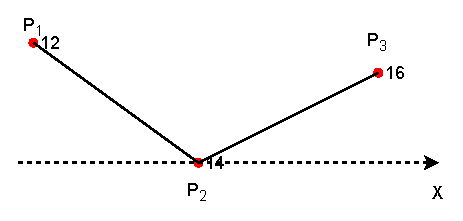
\includegraphics[width=0.9\linewidth]{angle}
\caption{角度计算图示}
\label{picture:25}
\end{figure}

由于经费有限,不失一般性,在本次实验中我们仅以右肘部单节点姿态模仿为例。对于全节点的机器人,我们只需按照单节点同样原理计算出多节点的角度并传到arduino开发板中即可。

最终效果如图~\ref{picture:26}~所示
\begin{figure}[!h]
\setlength{\subfigcapskip}{-1bp}
\centering
\begin{minipage}{\textwidth}
\centering
\subfigure{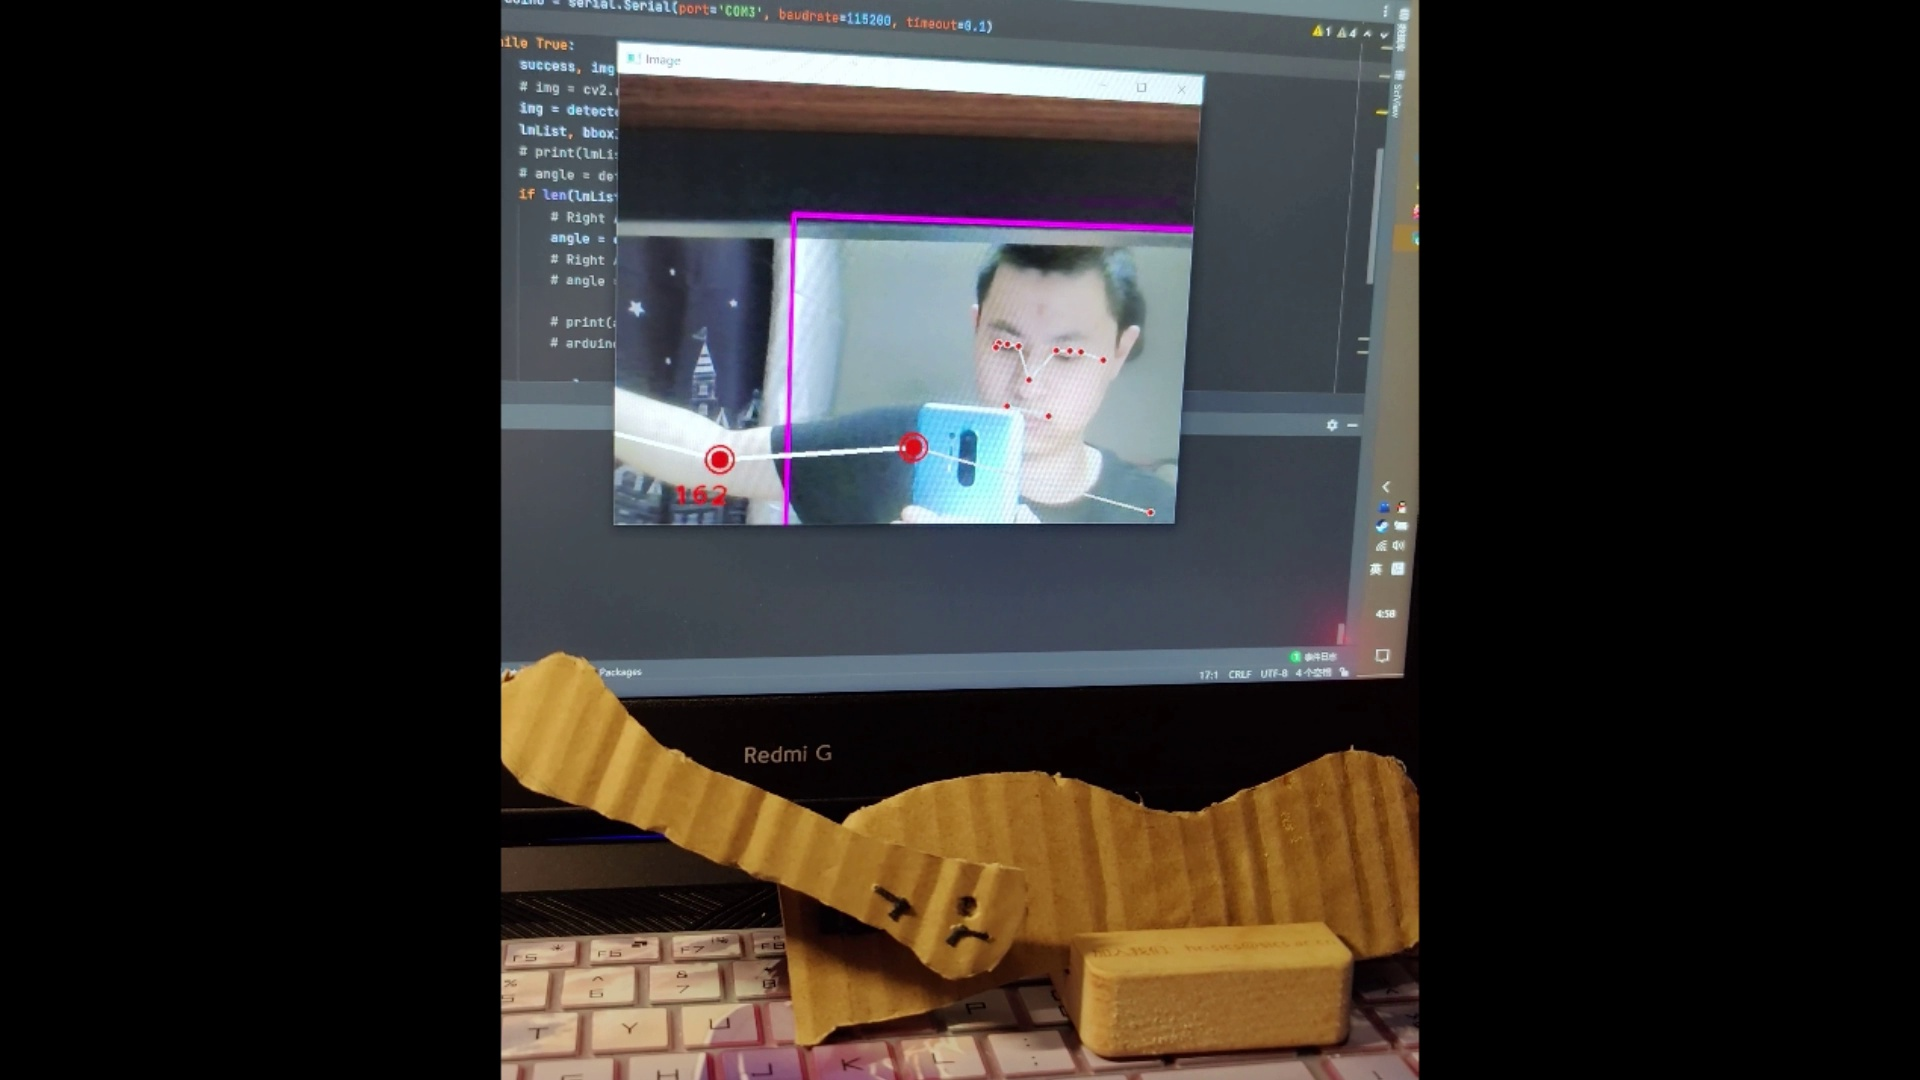
\includegraphics[width=0.31\textwidth]{robot1}}
\subfigure{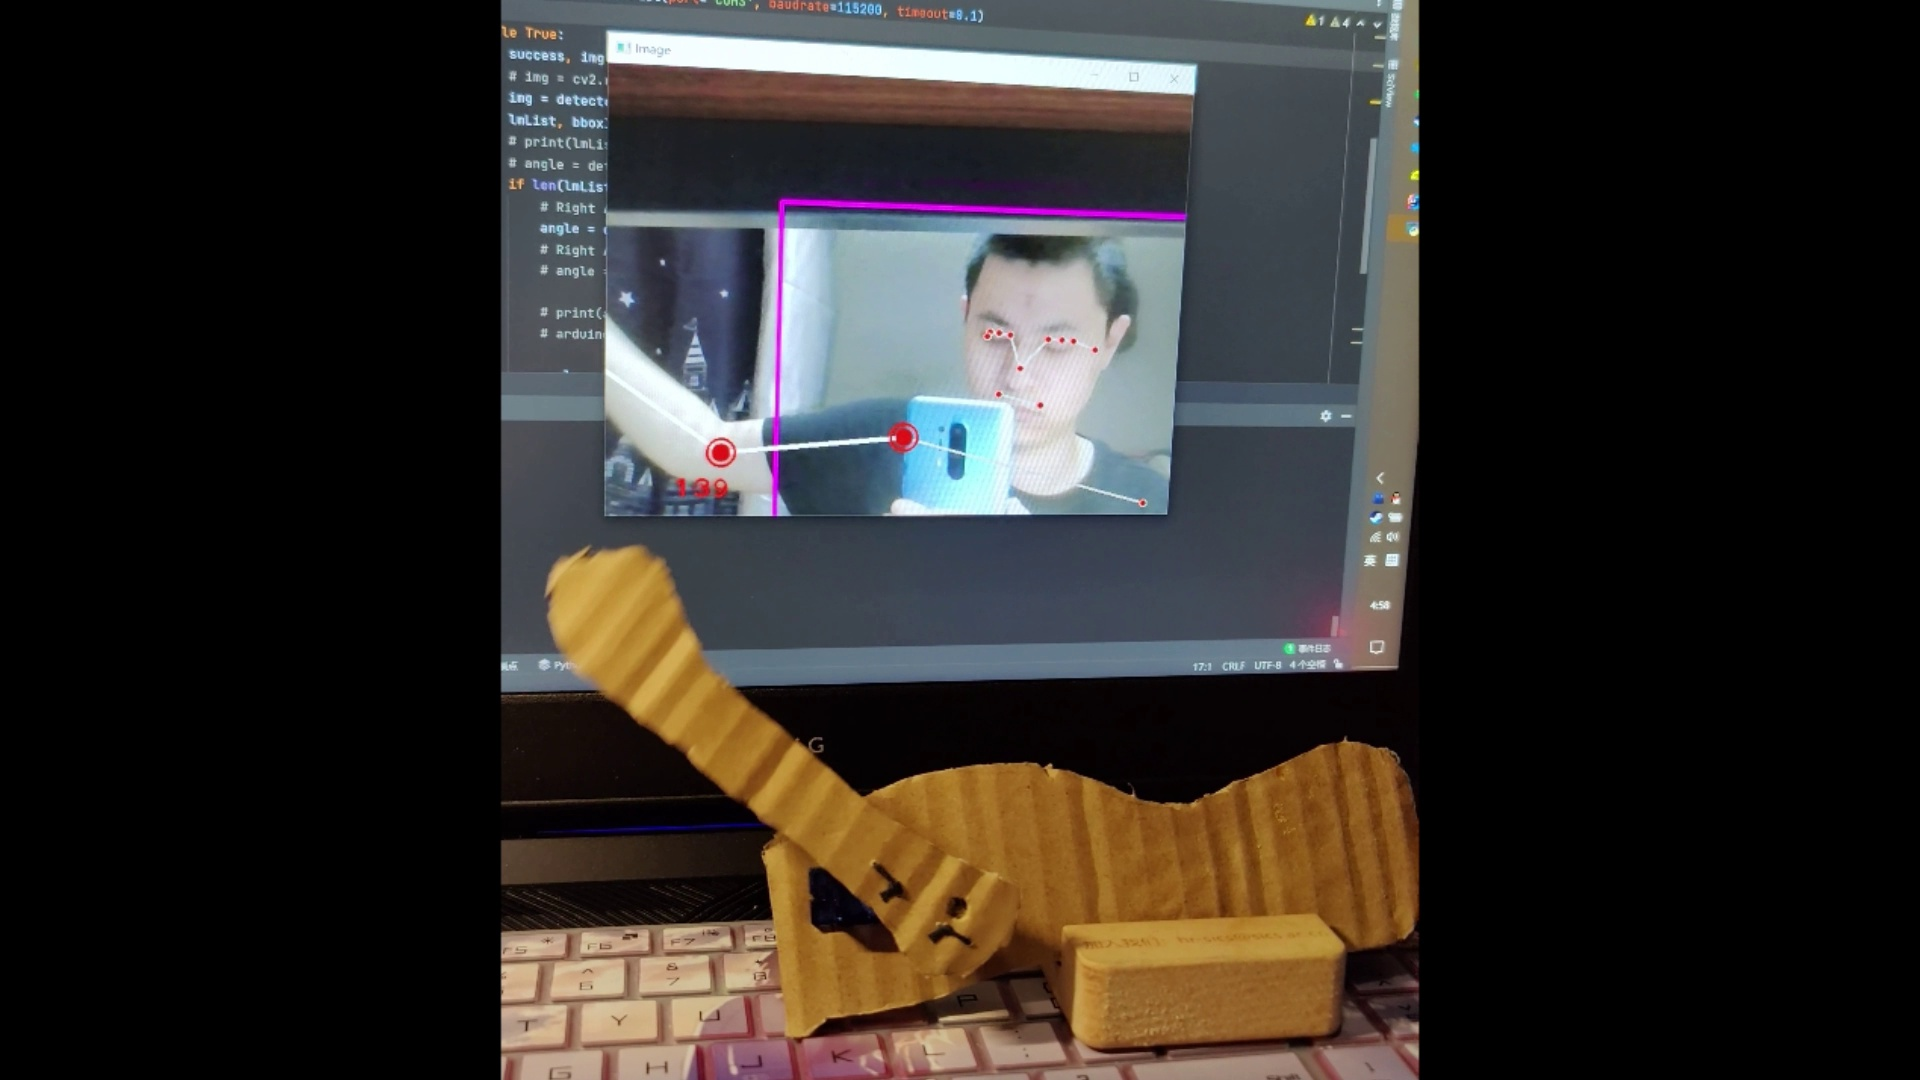
\includegraphics[width=0.31\textwidth]{robot2}}
\subfigure{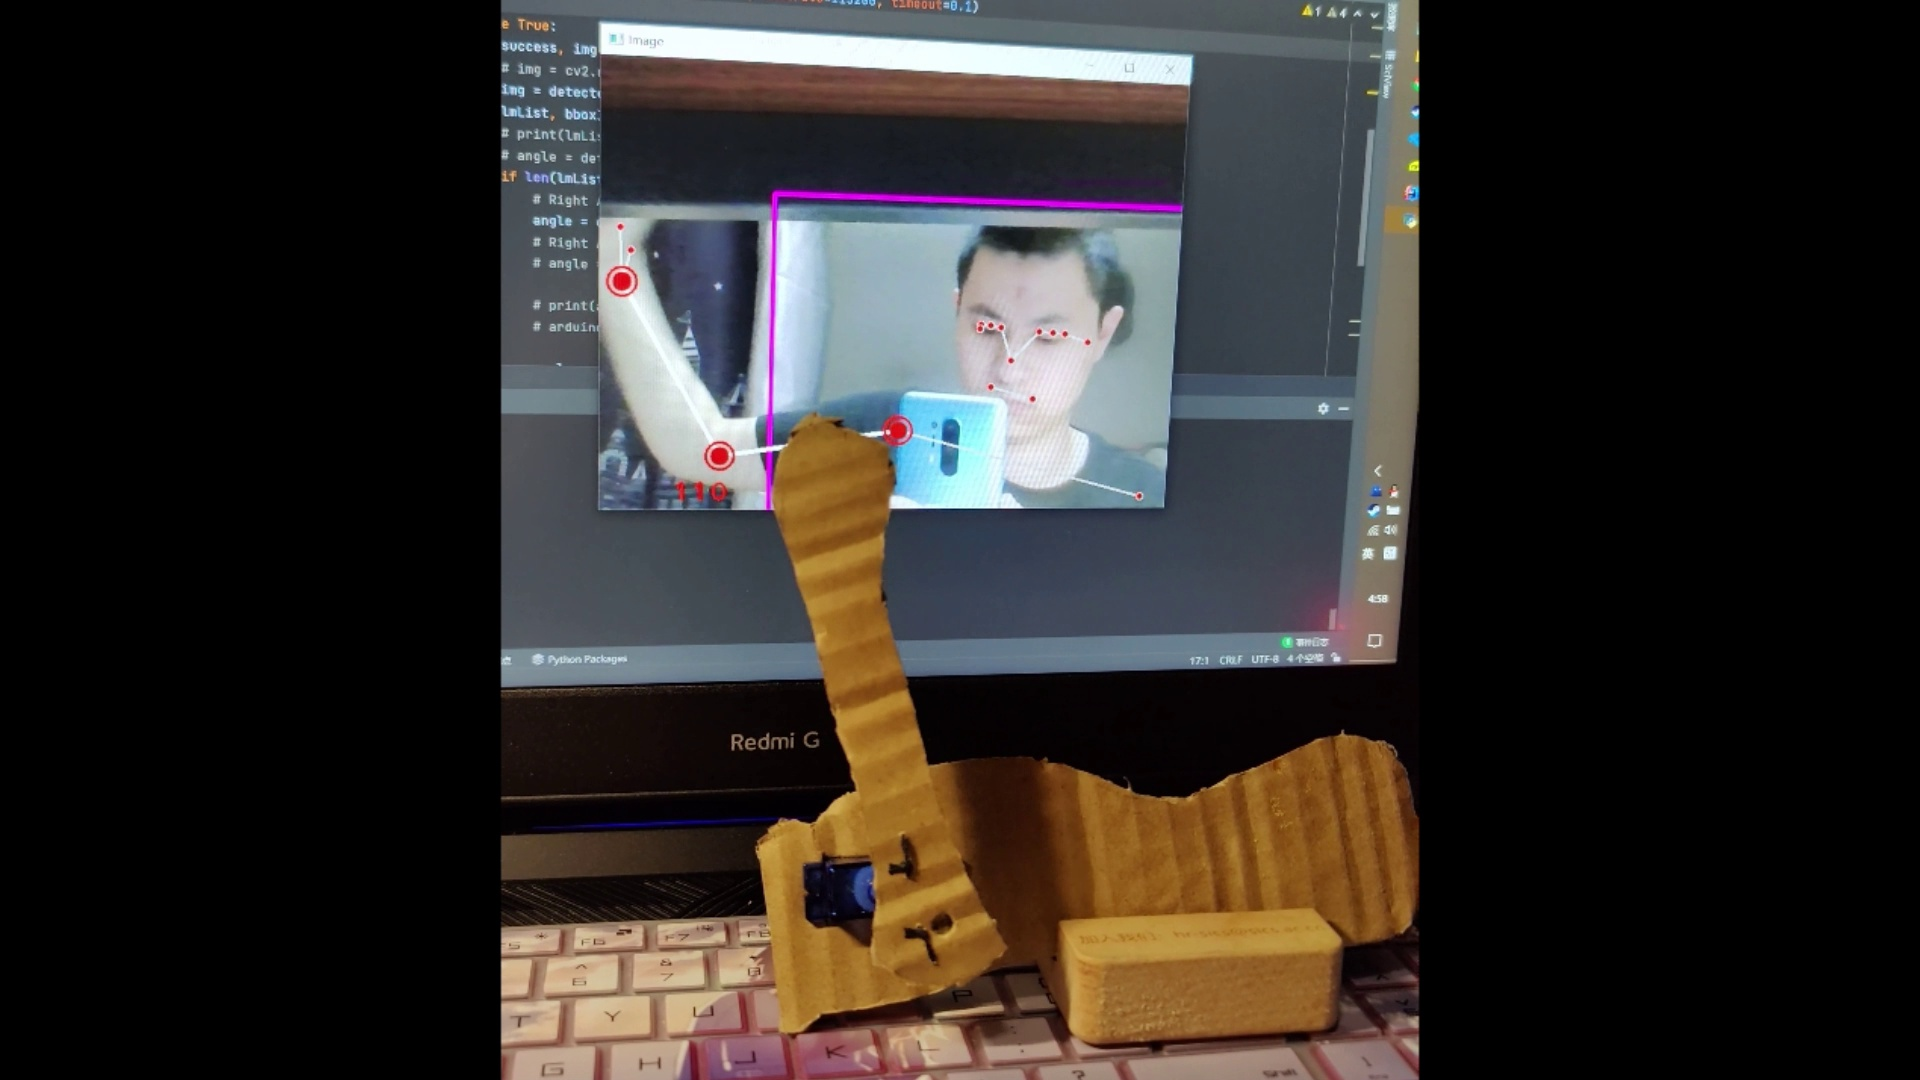
\includegraphics[width=0.31\textwidth]{robot3}}
\end{minipage}
\begin{minipage}{\textwidth}
\centering
\subfigure{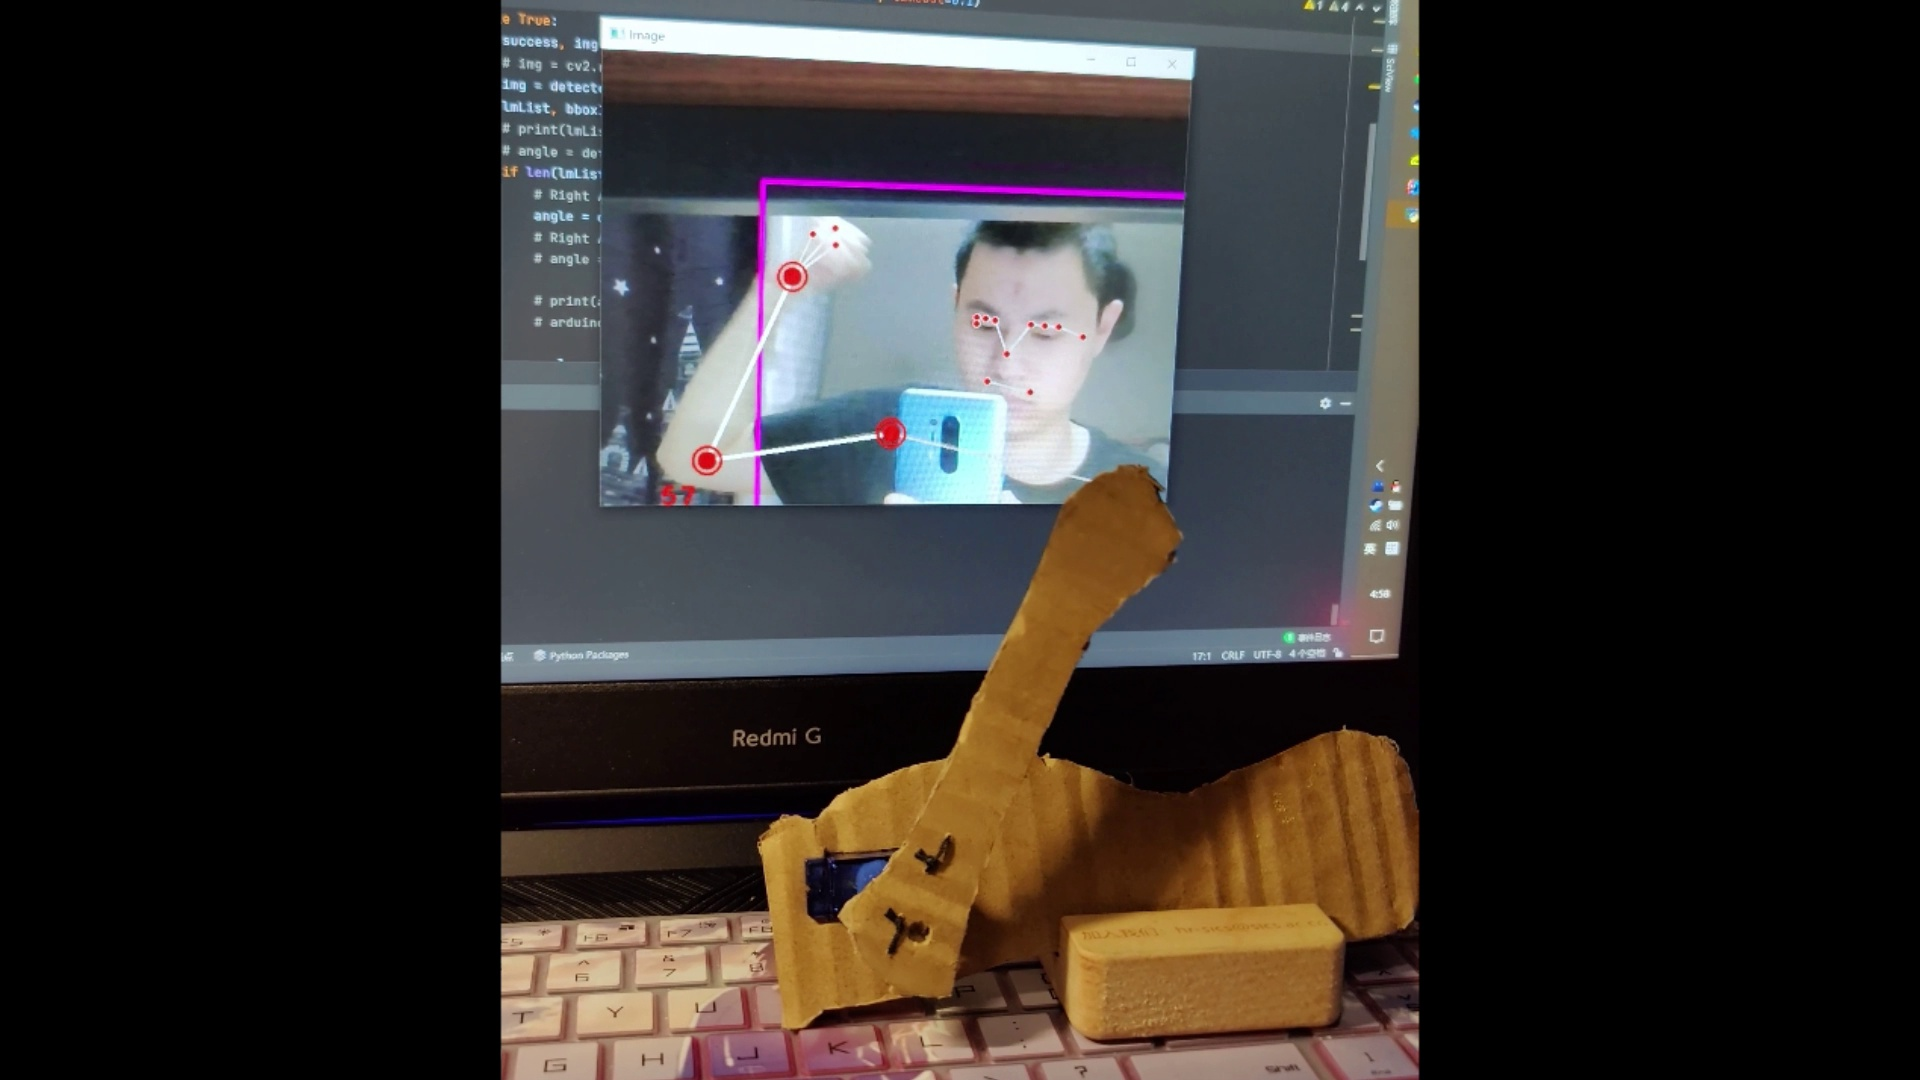
\includegraphics[width=0.31\textwidth]{robot4}}
\subfigure{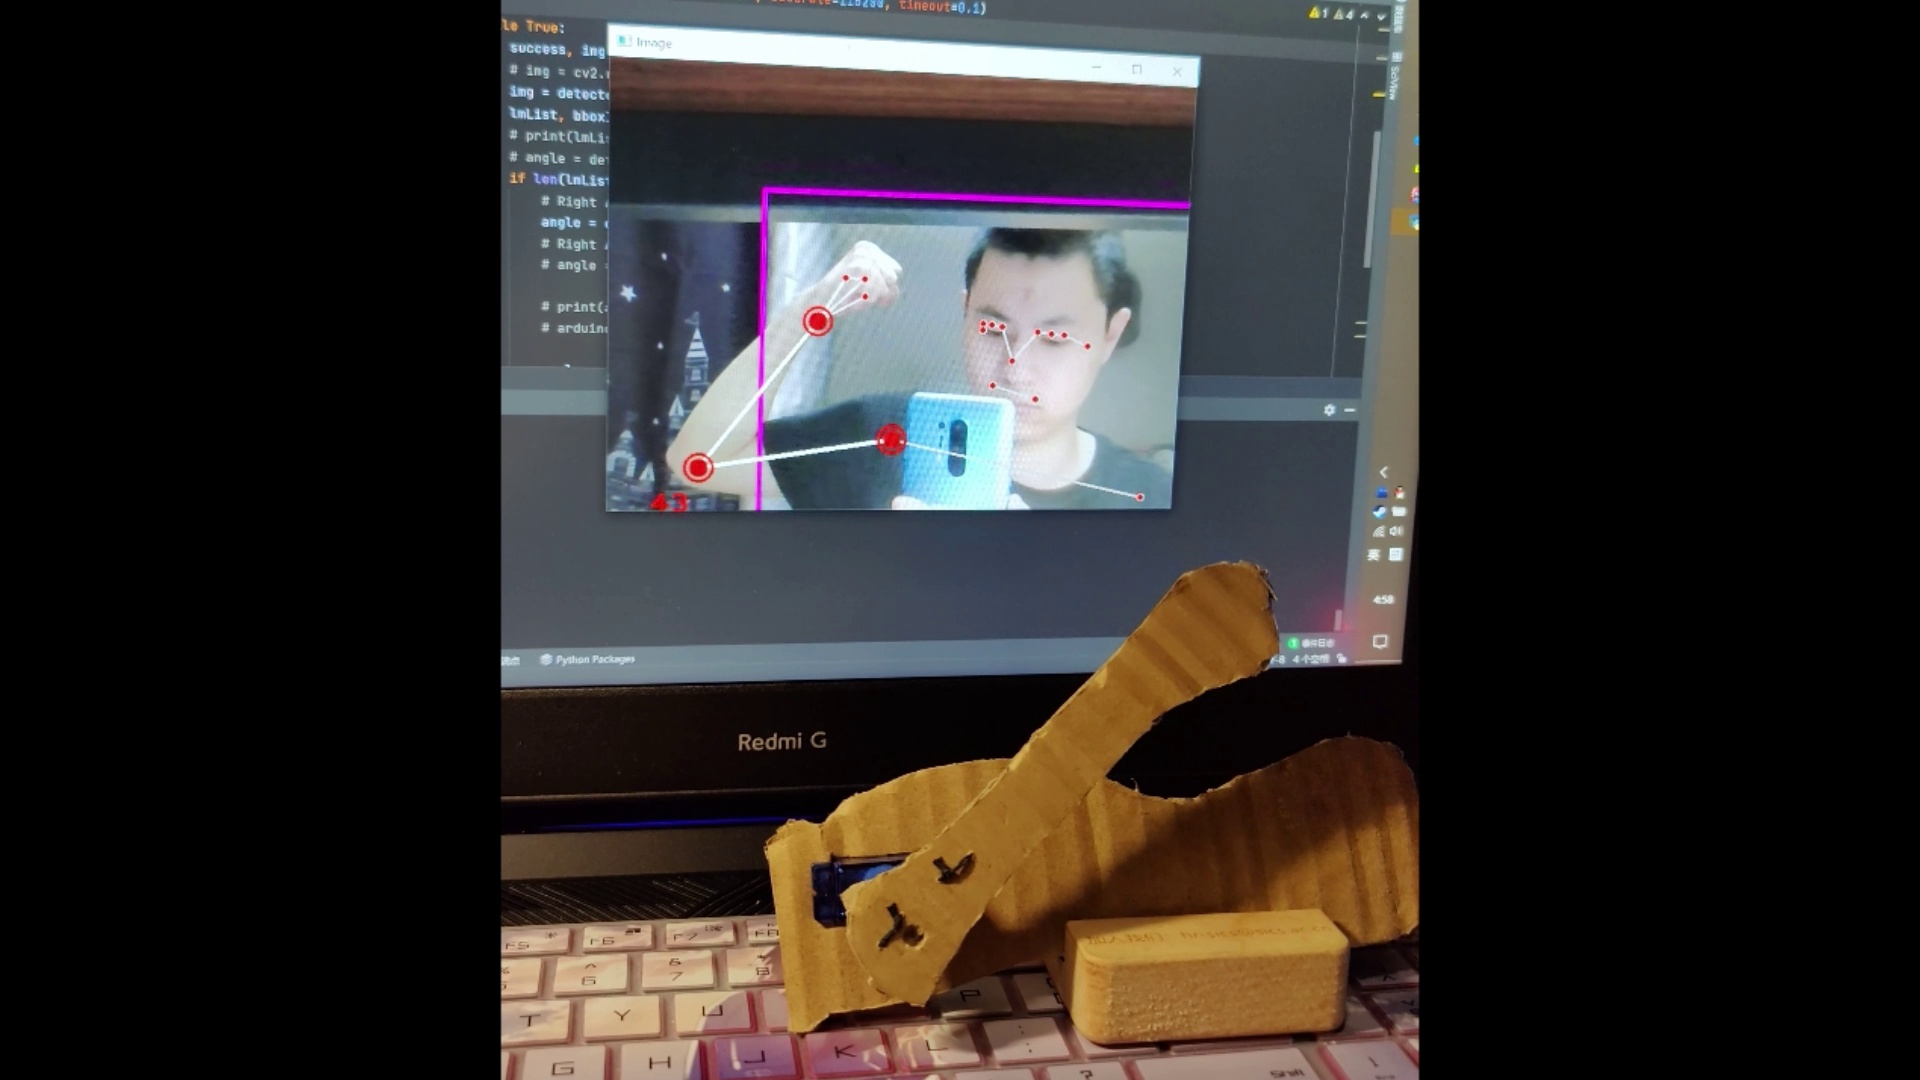
\includegraphics[width=0.31\textwidth]{robot5}}
\subfigure{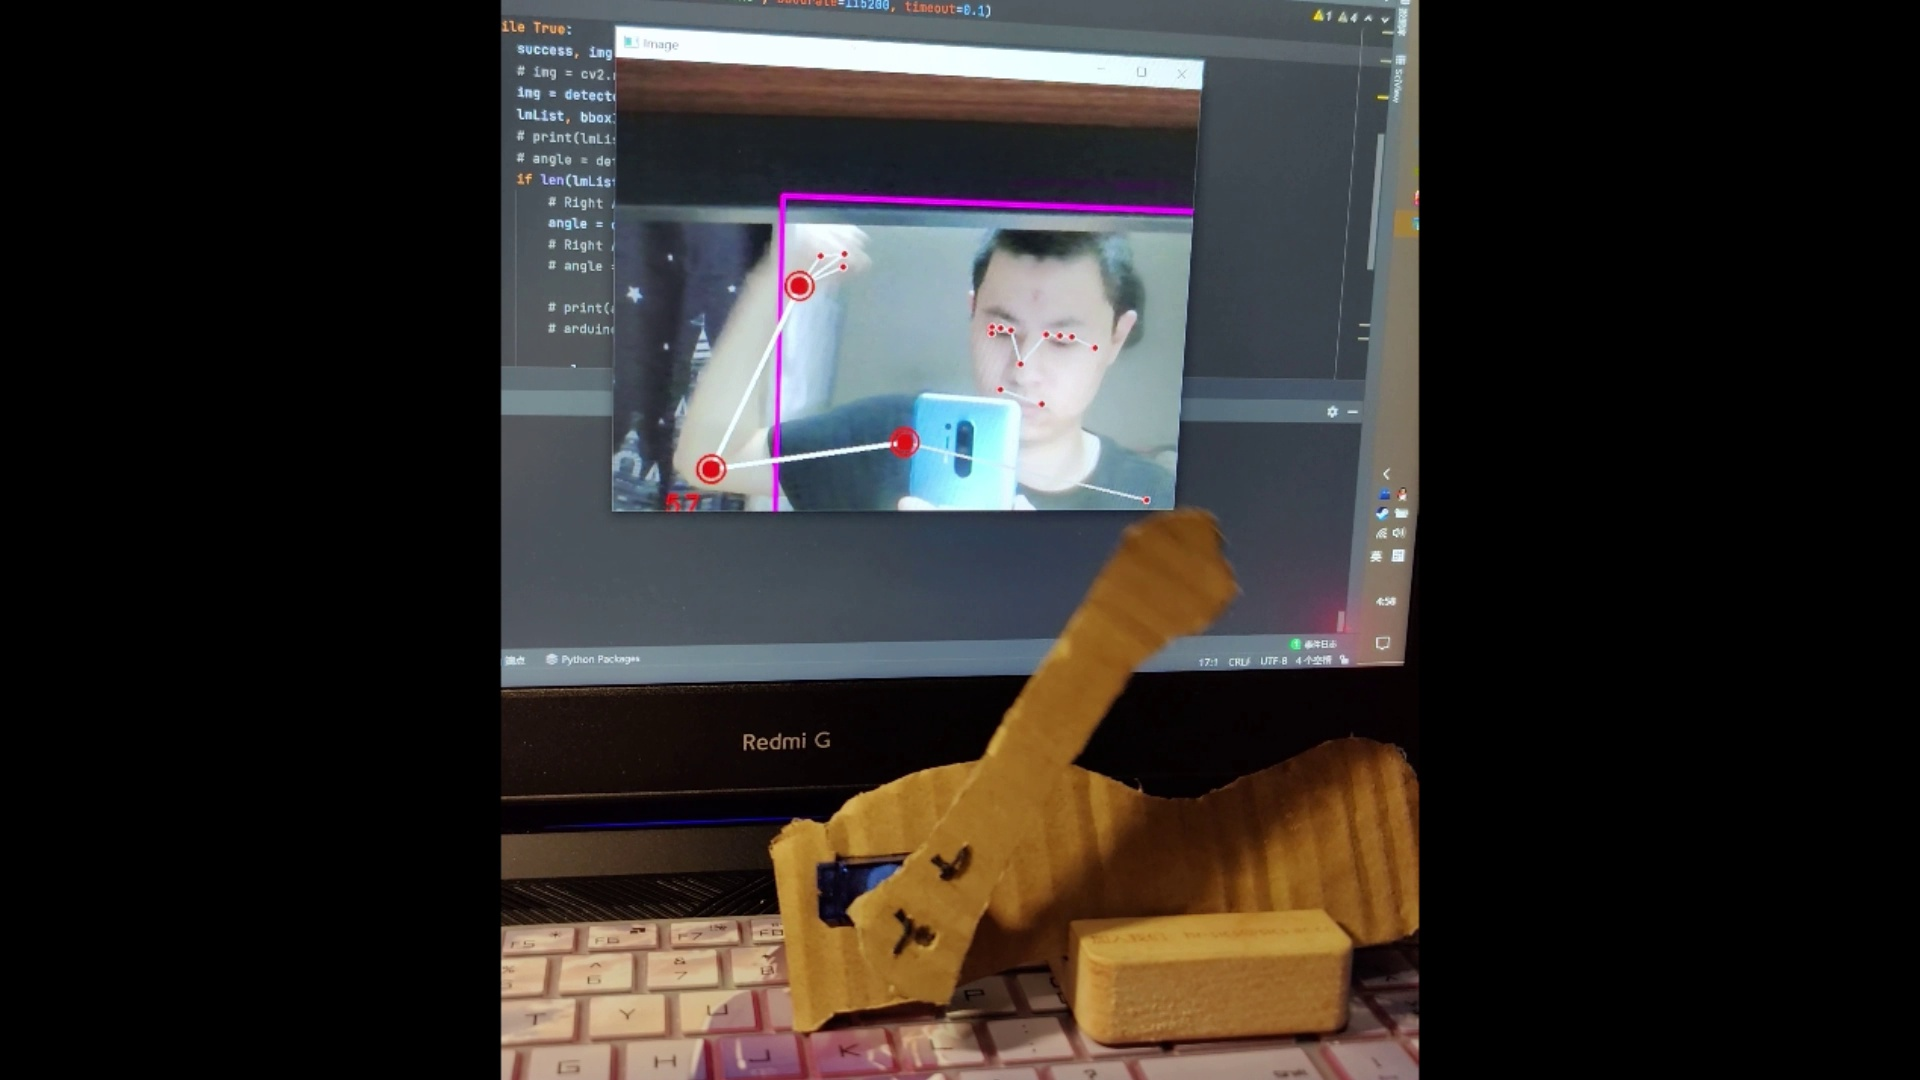
\includegraphics[width=0.31\textwidth]{robot6}}
\end{minipage}
\begin{minipage}{\textwidth}
\centering
\subfigure{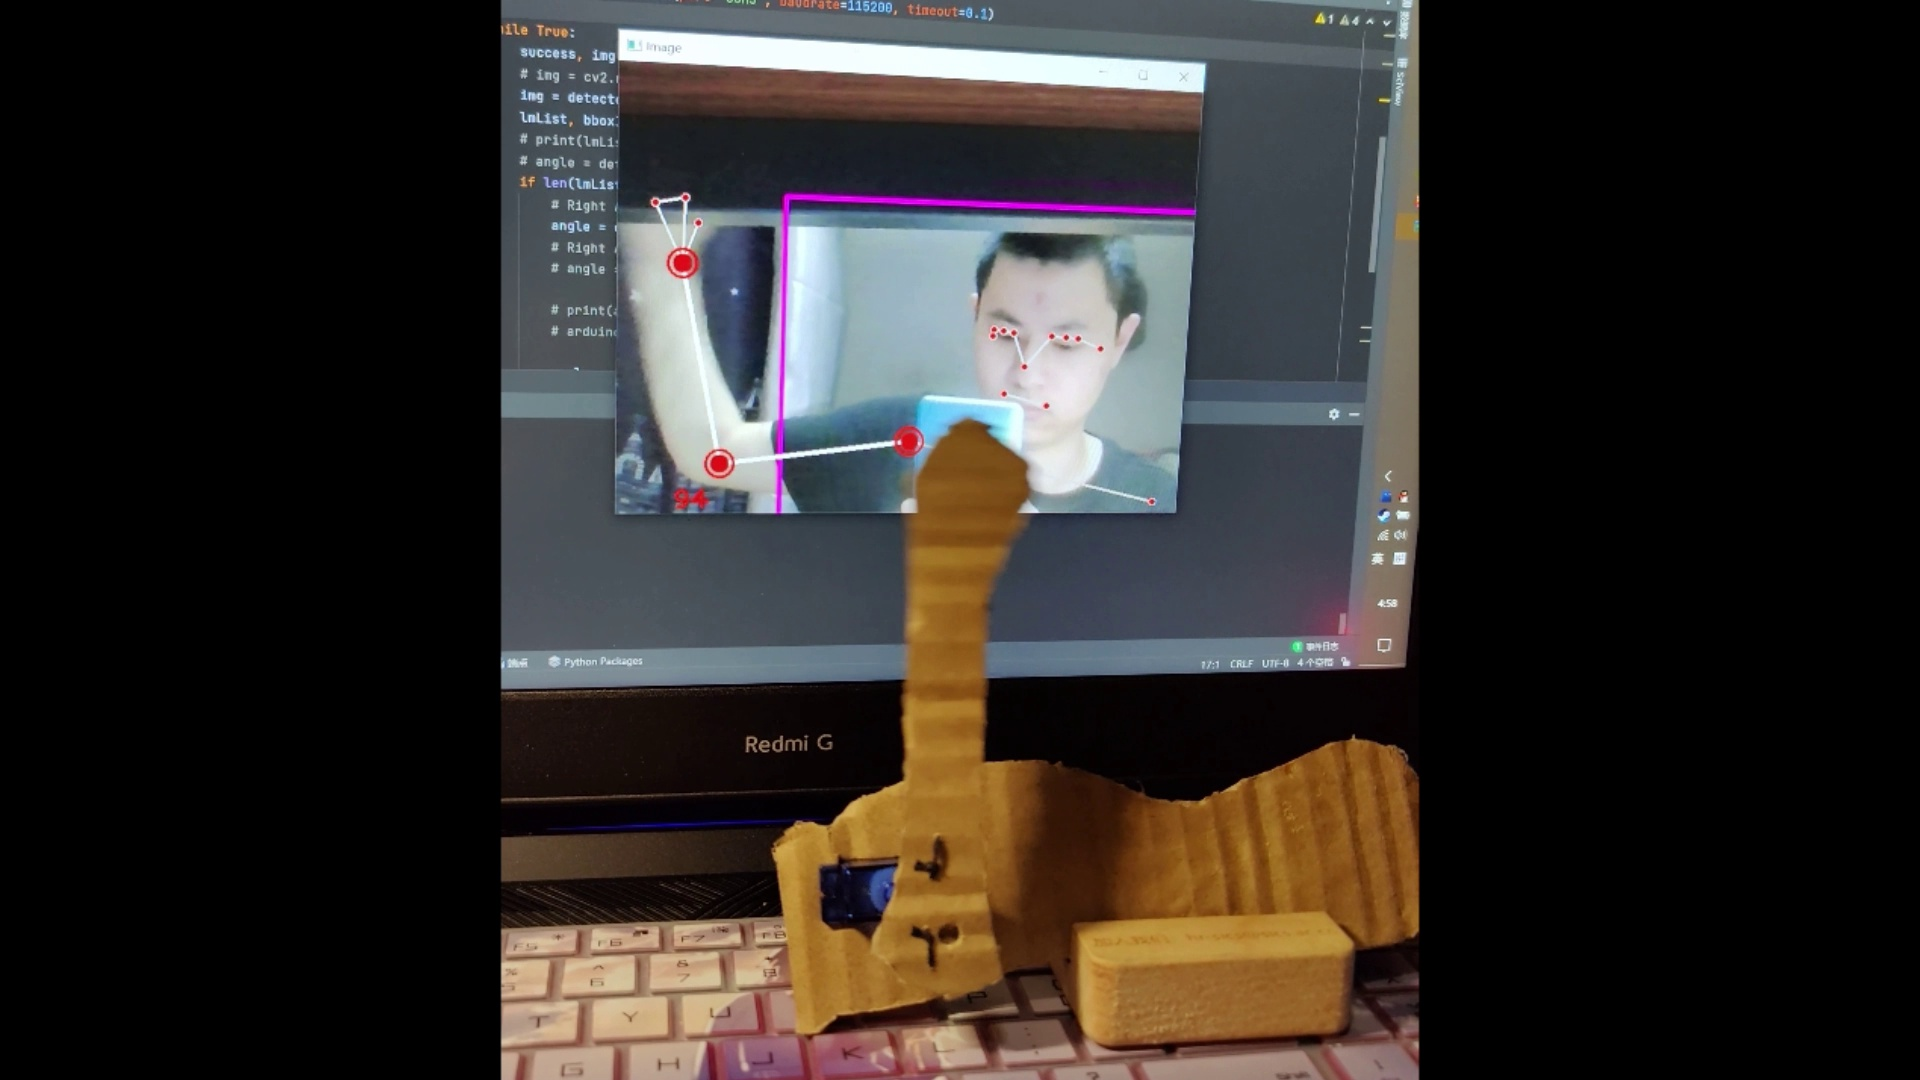
\includegraphics[width=0.31\textwidth]{robot7}}
\subfigure{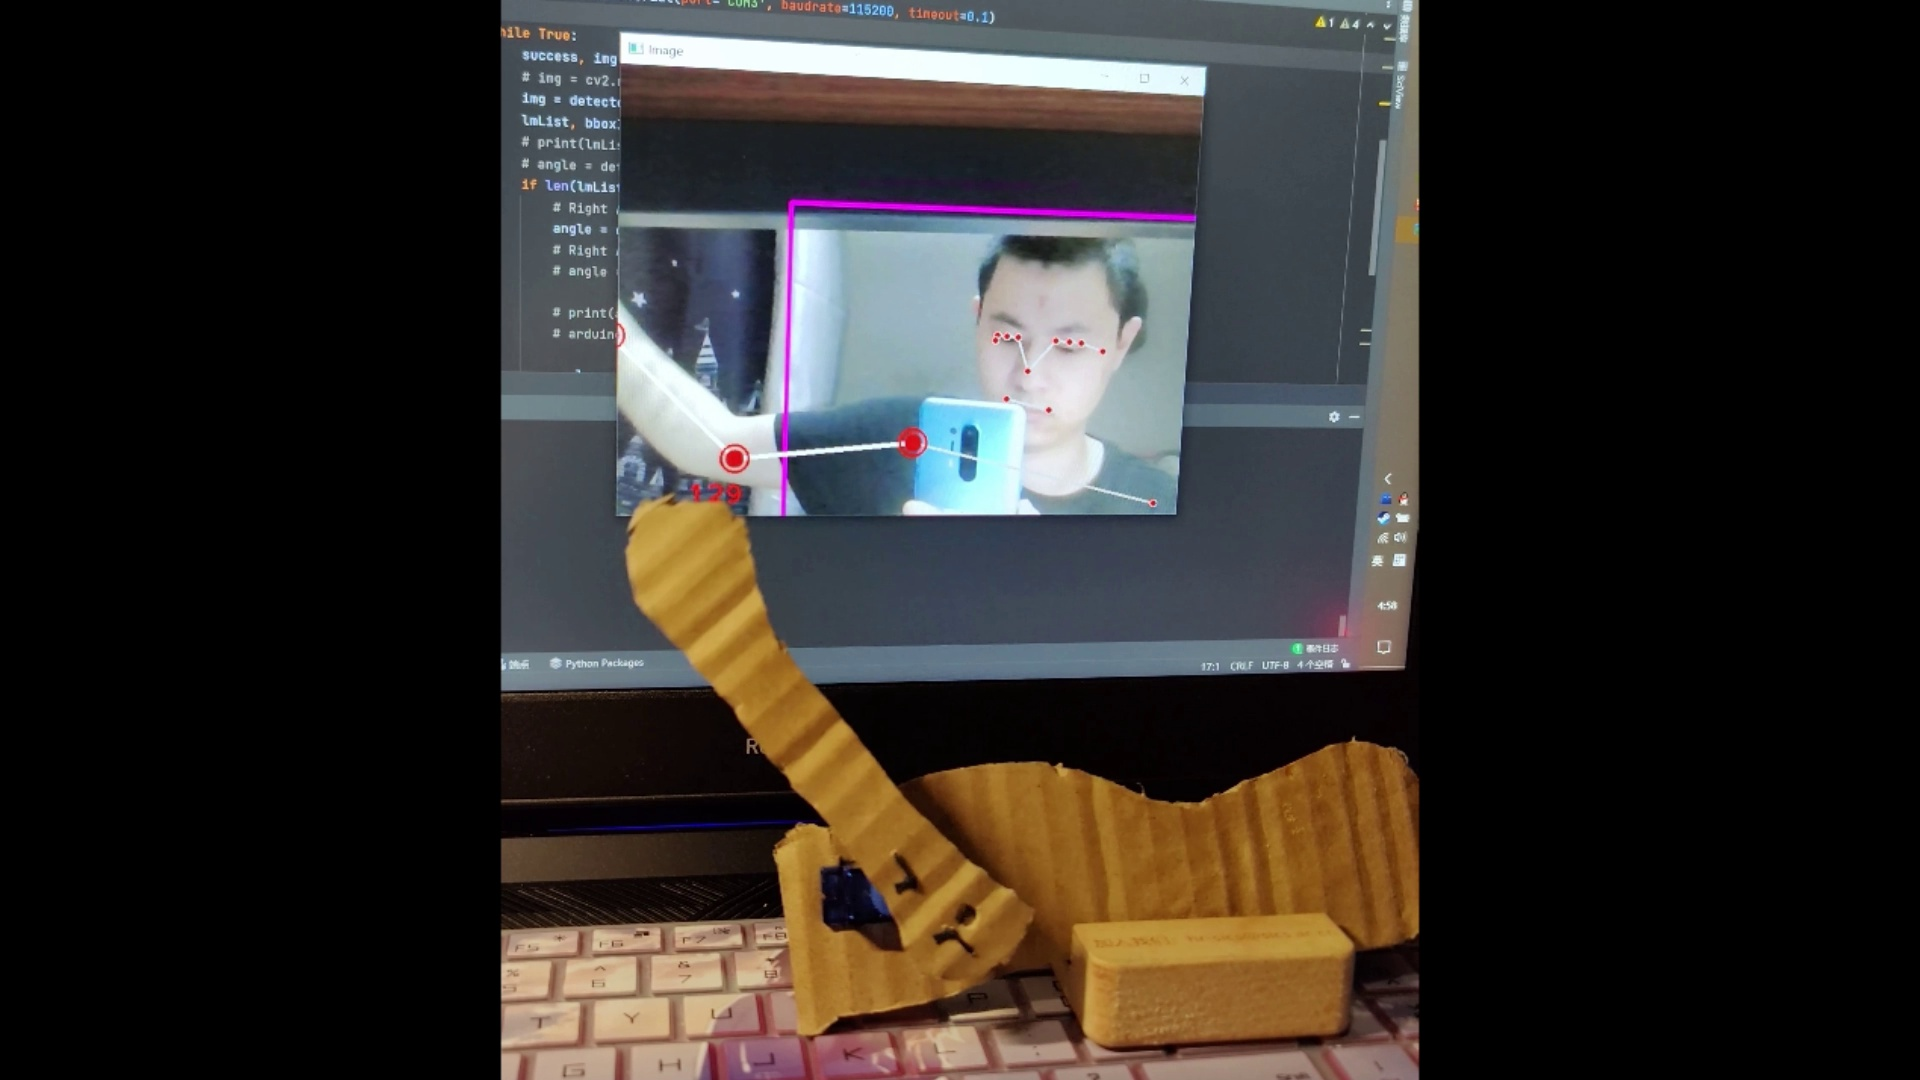
\includegraphics[width=0.31\textwidth]{robot8}}
\subfigure{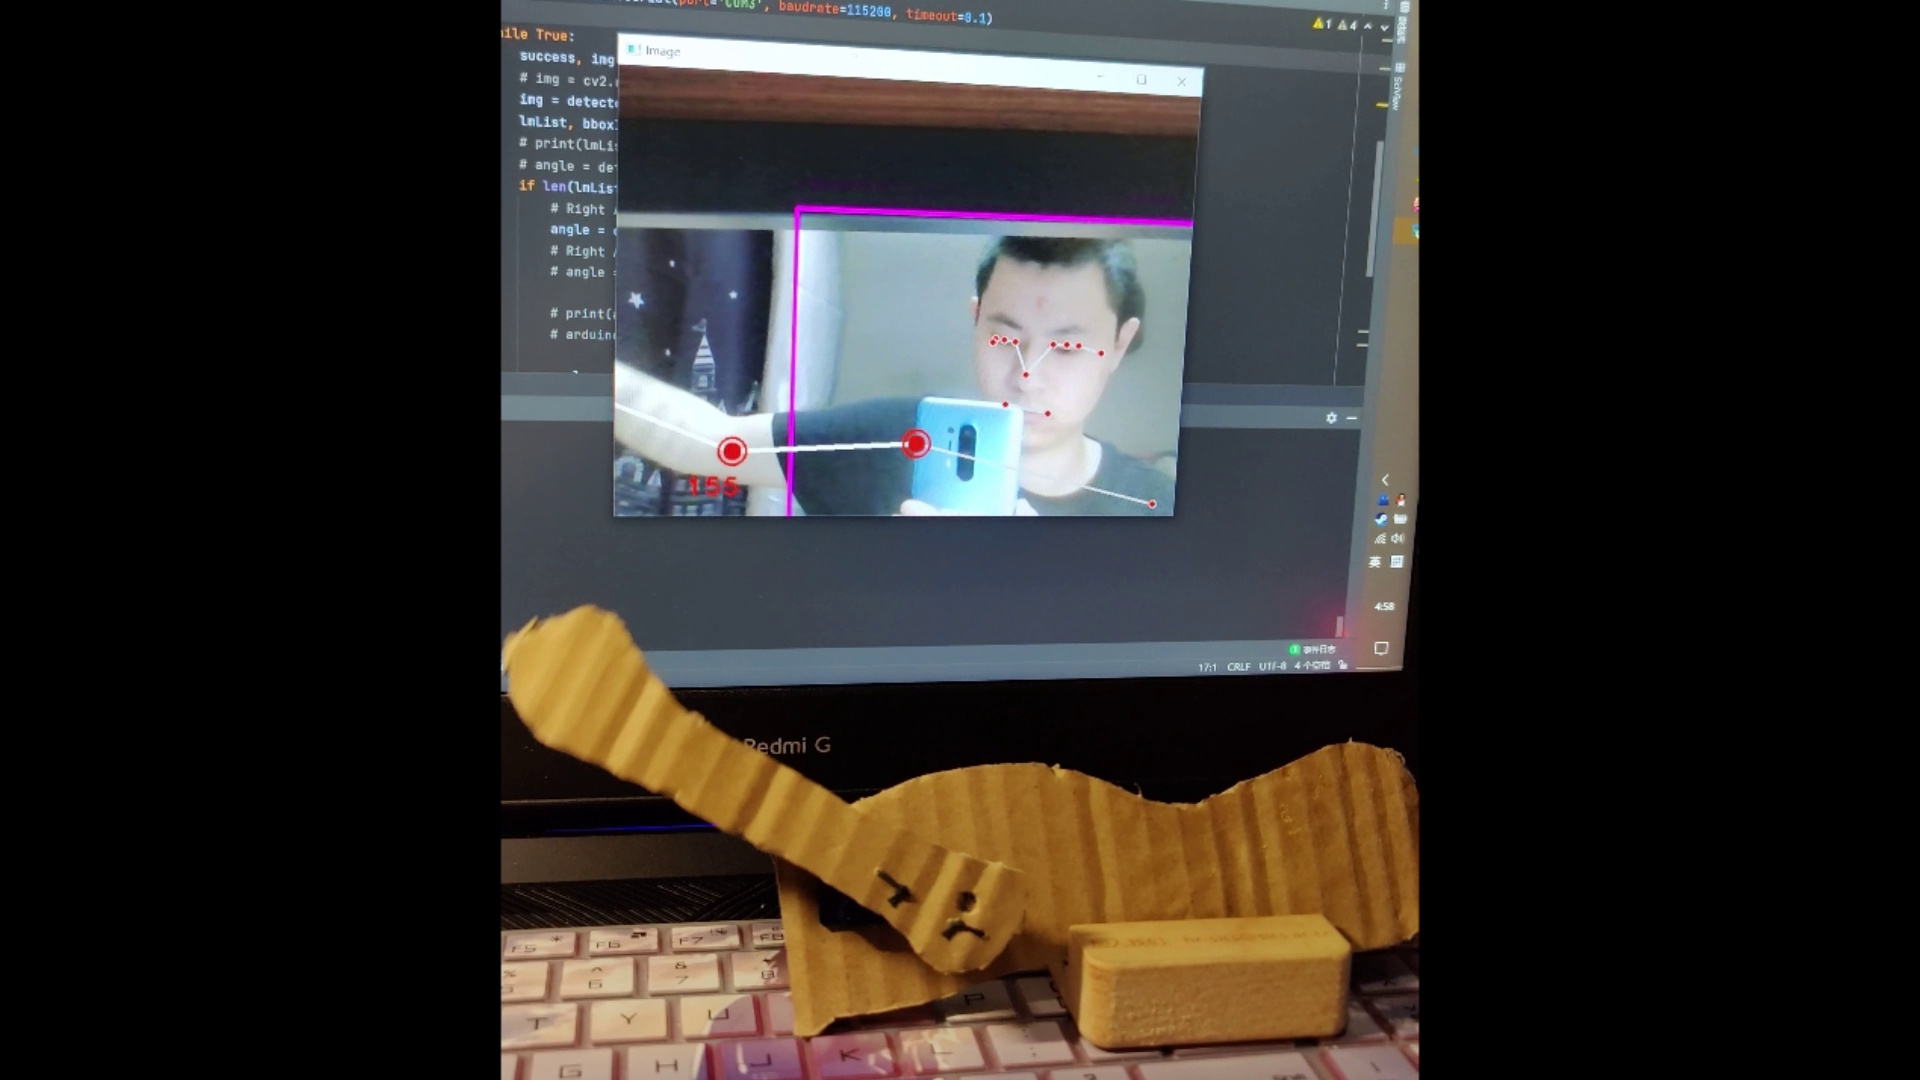
\includegraphics[width=0.31\textwidth]{robot9}}
\end{minipage}
\begin{minipage}{\textwidth}
\centering

\subfigure{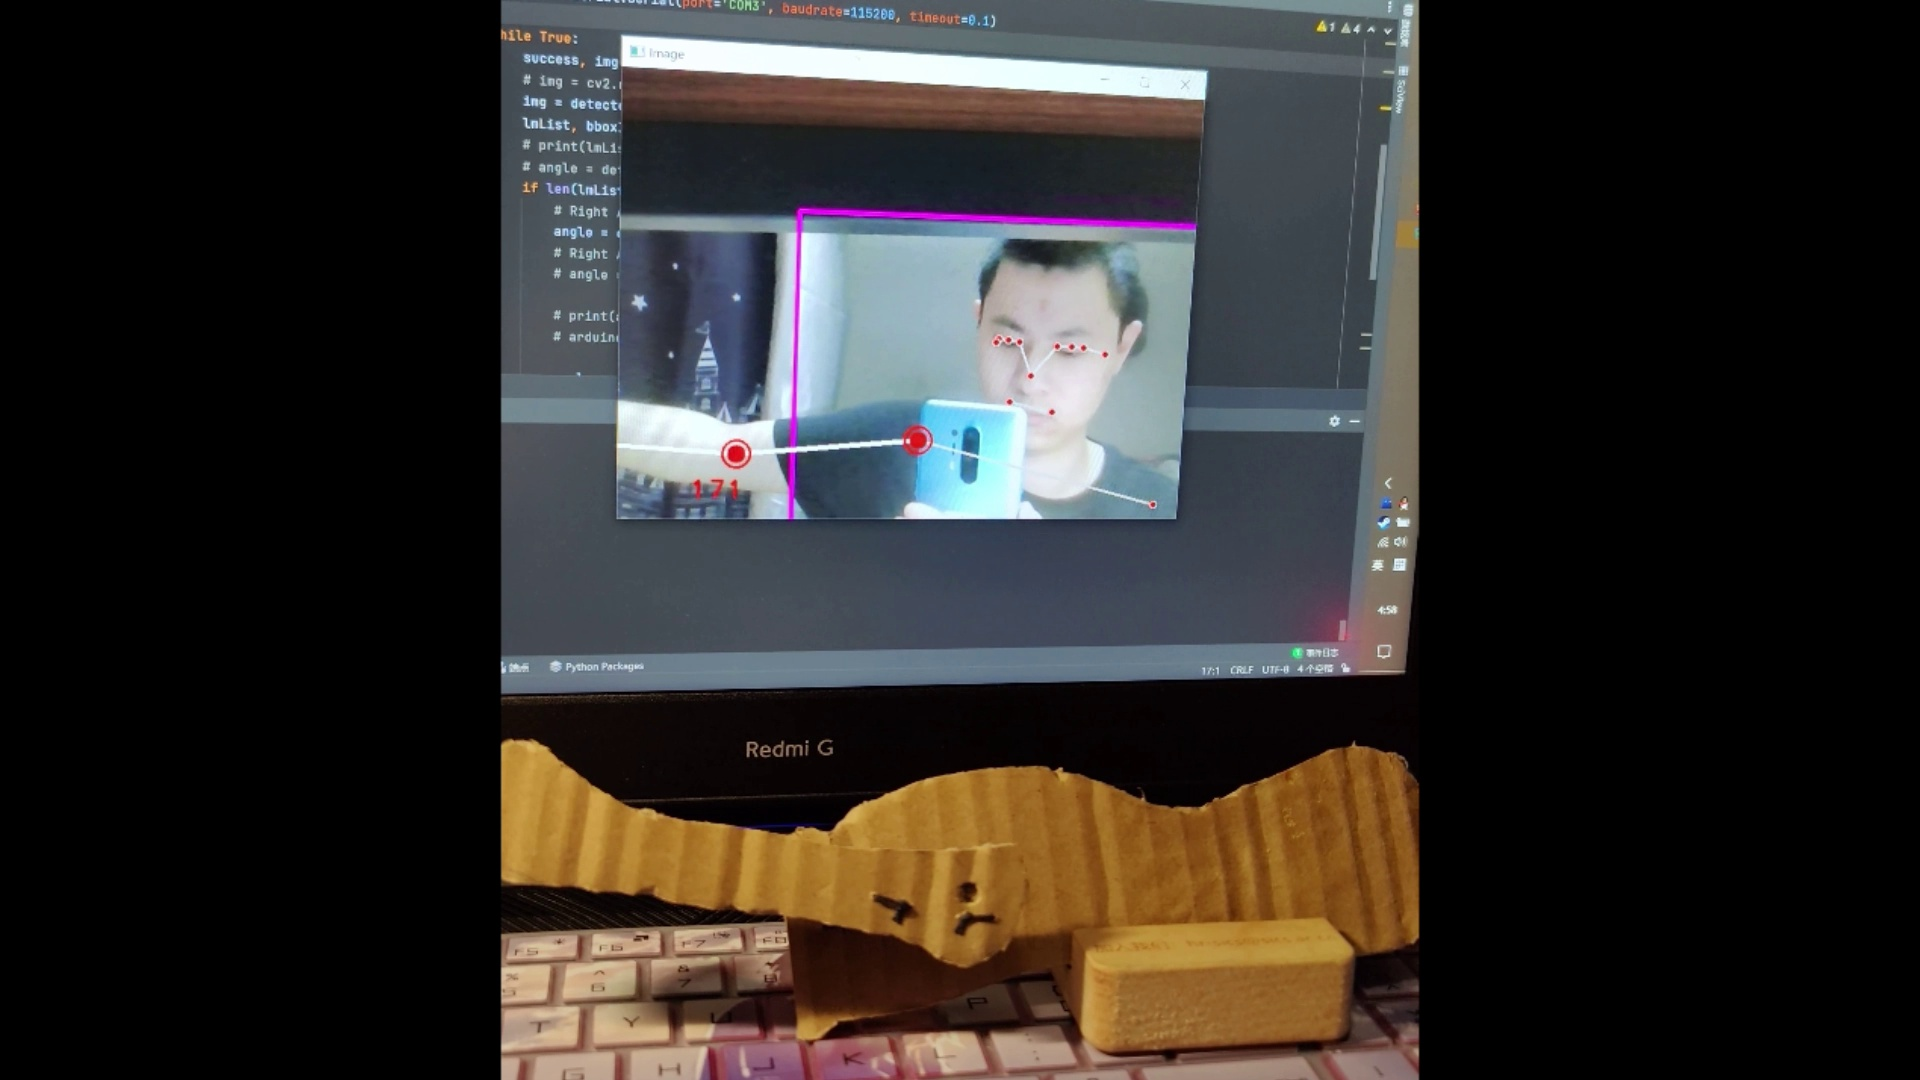
\includegraphics[width=0.31\textwidth]{robot10}}
\subfigure{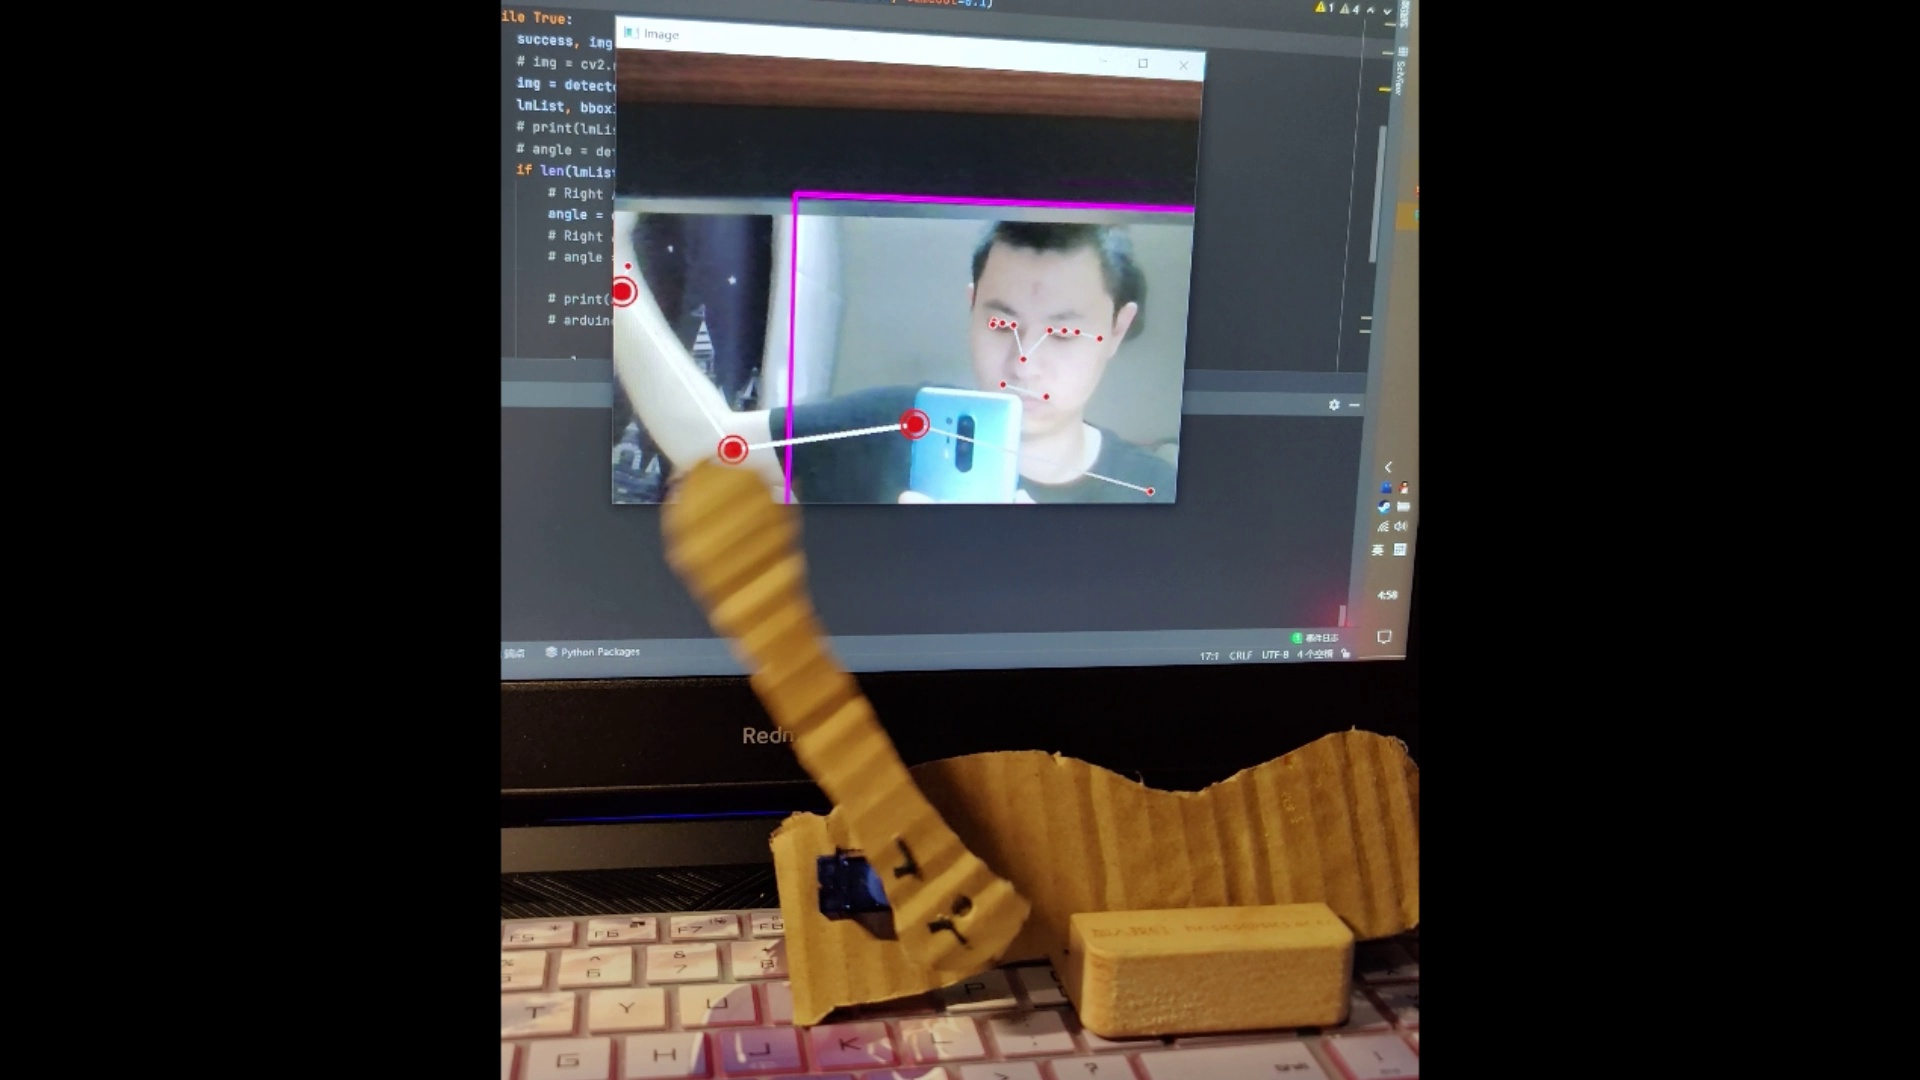
\includegraphics[width=0.31\textwidth]{robot11}}
\subfigure{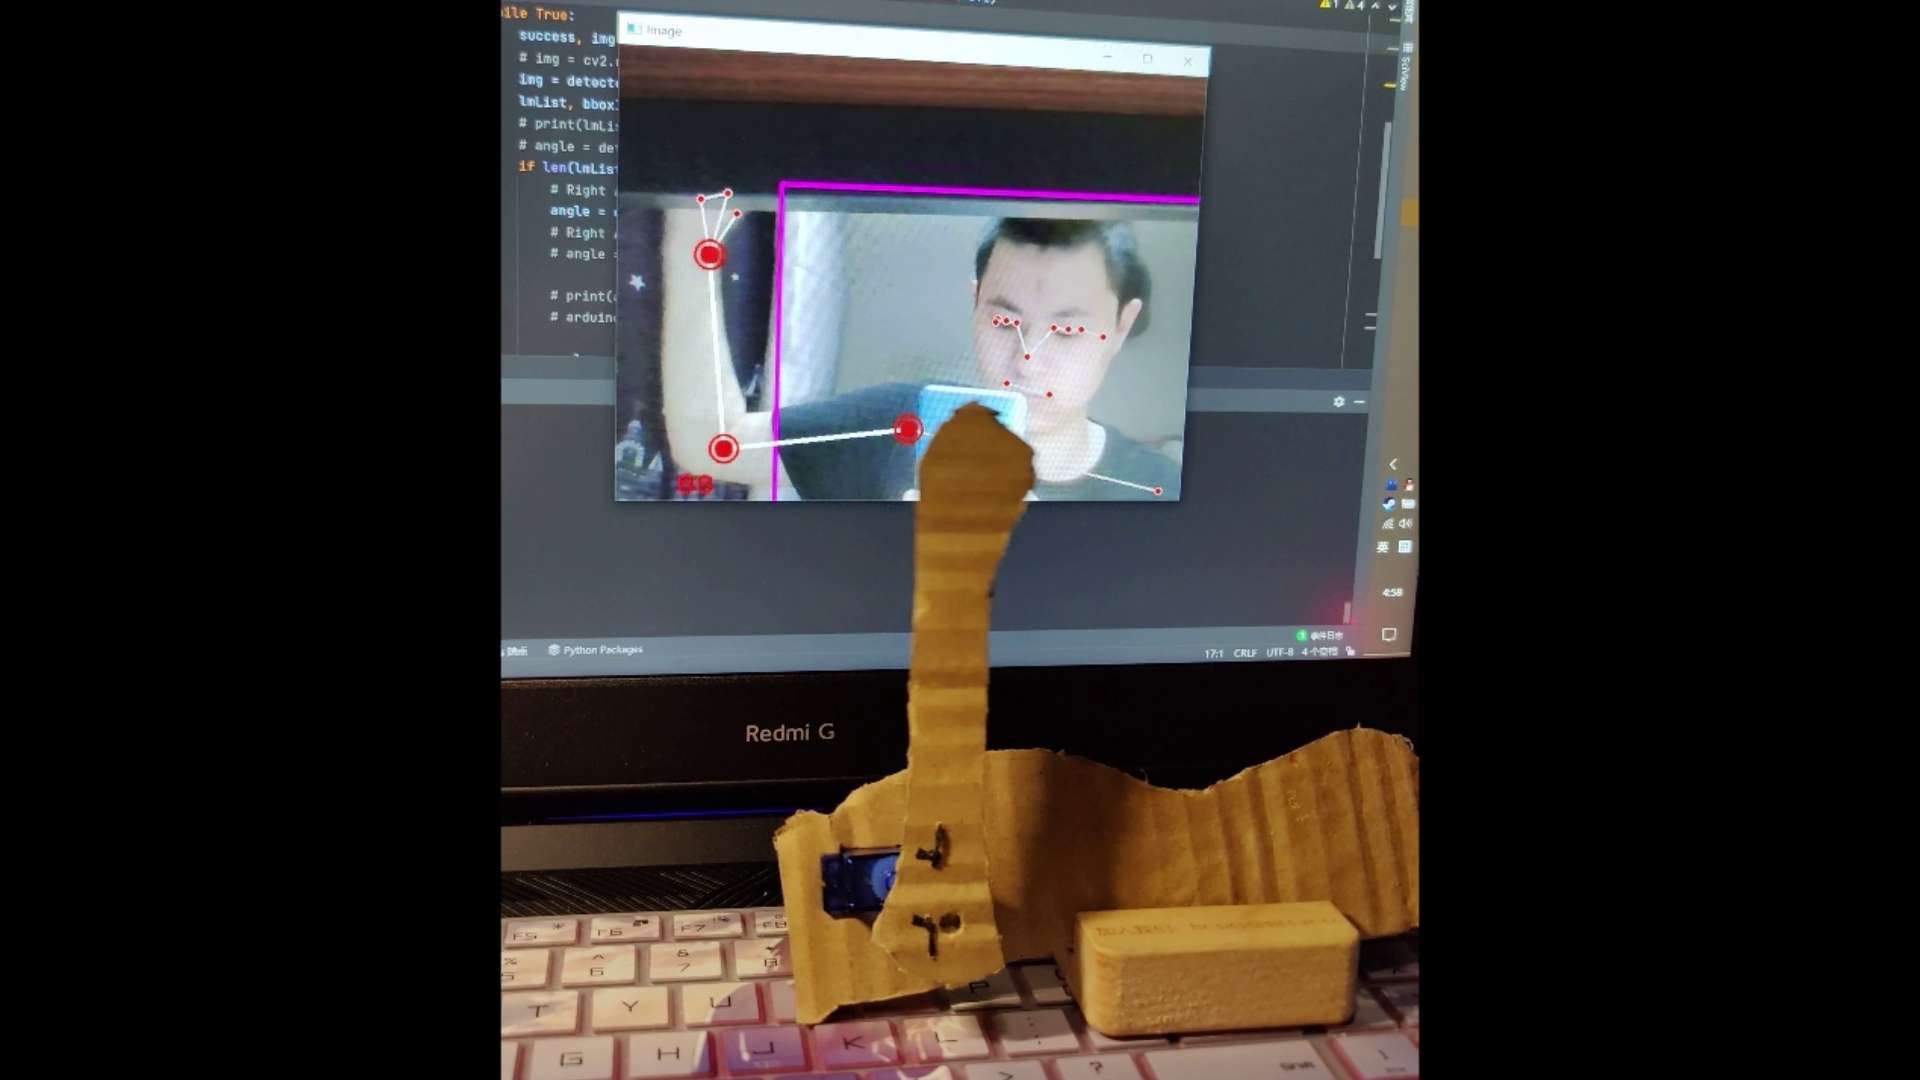
\includegraphics[width=0.31 \textwidth]{robot12}}
\end{minipage}
\vspace{0.2em}
\caption{真实机器人单右肘部姿态模仿截图}
\label{picture:26}
\end{figure}

从时间同步性以及动作准确度的角度来说,当摄像头读取的人体姿态发生变换的同时,机器人也会基本同步完成姿态转变。体现了本模型及时性和轻量化。进一步说明该模型已经达到实用的程度。

\section{本章小结}
本章是实验章节,主要是复现了BlazePose算法,并且将复现的模型与原版模型以及一些主流的模型进行了性能对比,在得到一个可以实用的模型后,本章又将其部署到了电脑端,移动端,虚拟机器人和真实机器人上。最后,得出结论:从机器人模仿的准确度和实时性而言,本项目以达到了预期的效果。


% Local Variables:
% TeX-master: "../main"
% TeX-engine: xetex
% End:

\backmatter
% !Mode:: "TeX:UTF-8" 
\begin{conclusions}

在本项目的结论中,我们首先概括论文的主要内容和贡献,然后对存在的不足之处提出展望。

单人姿态估计是视觉领域难度极大的研究方向之一。但在应用场景上,单人姿态估计表现出了极大的需求,虚拟试衣、智能安防、体育健身、VR技术等场景都亟需该算法的落地应用。

人机交互的主要目的是使机器人能够学习和了解人,能领会和模仿人的语言和行为。为了是人机交互自然,必须引入类似于人与人之间的沟通方式,即依赖语音与视觉。在这种背景下,人体姿态估计在人机交互方面有着举足轻重的作用。本文就是对此提出了基于人体姿态估计的机器人姿态跟踪算法,系统地完成了足够轻量化的人体姿态估计算法,并落实到了移动端,机器人端。具体的研究内容和研究成果如下:

\begin{enumerate}
\item 系统全面地介绍了人体姿态估计所涉及领域的主要内容,包括卷积神经网络的组成、反向传播算法、激活函数以及正则化。并且介绍了国内外对于单人姿态估计算法的发展历程以及各自的优势,为后续的BlazePose算法研究打下基础。

\item 研究了BlazePose算法,将目前最主流的基于热图的姿态估计和基于回归的姿态估计相结合。使用编码器-解码器网络架构来预测所有关节的热图。同时后面跟着另一个编码器,直接回归到所有关节的坐标。值得注意的是,热图分支可以在推理过程中被丢弃,使得网络足够轻量化,使得其可以架构在移动端和机器人端。

\item 在目标检测的后处理步骤中,不使用NMS算法,而是假设人脸这一相对刚性的目标一直会出现。因为多个不明确的框满足NMS算法的交并集(IoU)阈值,而人脸检测器则打破了这一限制。

\item 同时我们拓展了现在比较基础的17的关键点,增加至33个关键点,使得模型所表达的语义信息更加丰富,以便于可以用到更复杂的应用场景。

\item 然后,我们还对比了重构的模型与官方模型以及其它模型的性能,结果显示,重构模型的准确率能达到82.5\%,并且在帧数上也远超OpenPose接近官方模型。

\item 最后,我们一步步将模型部署到电脑端,移动端,虚拟机器人以及真实机器人上。从时间同步性以及动作准确度的角度来说,该模型已经达到实用的程度。
\end{enumerate}

本次研究复现的模型虽然达到了一定的效果,但依然存在一些局限性,结合市场需求以及国内外目前研究内容,对该模型作出如下展望:

\begin{enumerate}
\item 进一步提高模型的轻量化和性能,使得模型能在部署在性能较差的机器人上,并且使得机器人处理更加复杂的动作,改善交互体验。

\item 该模型是2.5D模型,虽然拥有着Z轴的分量,但是语义信息的损失极大,如何在保证模型轻量化的同时提高Z轴分量信息的准确度是一大难题。

\item 人体动作关键帧的准确提取。机器人通过自身的视觉系统捕获人体动作序列帧时,不用对每一帧图像进行处理,只需处理关键帧,其余的帧通过插值的方法估计出即可。如何得到这些动作关键帧需要进一步研究。
\end{enumerate}

\end{conclusions}
   % 结论
\bibliographystyle{gbt7714-numerical}
\bibliography{reference}
%%%%%%%%%%%%%%%%%%%%%%%%%%%%%%%%%%%%%%%%%%%%%%%%%%%%%%%%%%%%%%%%%%%%%%%%%%%%%%%% 
%-- 注意:以下本硕博、博后书序不一致 --%
%%%%%%%%%%%%%%%%%%%%%%%%%%%%%%%%%%%%%%%%%%%%%%%%%%%%%%%%%%%%%%%%%%%%%%%%%%%%%%%% 
% 硕博书序
%%%%%%%%%%%%%%%%%%%%%%%%%%%%%%%%%%%%%%%%%%%%%%%%%%%%%%%%%%%%%%%%%%%%%%%%%%%%%%%% 
%\begin{appendix}%附录
%% -*-coding: utf-8 -*-
%%%%%%%%%%%%%%%%%%%%%%%%%%%%%%%%%%%%%%%%%%%%%%%%%%%%%%%%%
\chapter{BlazePose各关键点的名称}
\label{keypoints}
%%%%%%%%%%%%%%%%%%%%%%%%%%%%%%%%%%%%%%%%%%%%%%%%%%%%%%%%%
\begin{table}[htbp]
\caption{BlazePose各关键点的名称}
\label{keypointstable}
\vspace{0.5em}\centering\wuhao
\begin{tabular}{cc}
\toprule[1.5pt]
关键点序号 & 关键点名称  \\
\midrule[1pt]
0 & 鼻子  \\
1 & 左眼内侧  \\
2 & 左眼  \\
3 & 左眼外侧  \\
4 & 右眼内侧  \\
5 & 右眼  \\
6 & 右眼外侧  \\
7 & 左耳  \\
8 & 右耳  \\
9 & 嘴巴左部  \\
10 & 嘴巴右部  \\
11 & 左肩  \\
12 & 右肩  \\
13 & 左肘  \\
14 & 右肘  \\
15 & 左手腕  \\
16 & 右手腕  \\
17 & 左小指 \\
18 & 右小指  \\
19 & 左手  \\
20 & 右手  \\
21 & 左拇指  \\
22 & 右拇指  \\
23 & 左髋关节  \\
24 & 右髋关节  \\
25 & 左膝  \\
26 & 右膝  \\
27 & 左脚踝  \\
28 & 右脚踝  \\
29 & 左脚后跟  \\
30 & 右脚后跟  \\
31 & 左脚  \\
32 & 右脚 \\
\bottomrule[1.5pt]
\end{tabular}
\end{table}

%\end{appendix}
%\include{back/publications}    % 所发文章
%\include{back/ceindex}    % 索引, 根据自己的情况添加或者不添加,选择自动添加或者手工添加。
%\authorization %授权
%%\authorization[scan.pdf] %添加扫描页的命令,与上互斥
%% !Mode:: "TeX:UTF-8"
\begin{acknowledgements}

光阴似箭,转眼已在哈尔滨工业大学度过了四年本科生涯。在这段时间里,我通过自己的努力学习,以及老师同学的帮助,完成了这篇毕业设计,为自己的本科生生涯交了一份美好的答卷。

衷心感谢导师傅忠传老师对本人的精心指导。感谢他的包容,给予我足够的自由来选择感兴趣的研究话题。也感谢他在我研究困难的时候给予我耐心,有效的指导,同时也感谢傅老师在时间安排方面,论文撰写方面给予我的宝贵意见。千言万语道不尽,只能在此对他道以最真诚的感谢。

此外,也要感谢哈工大\LaTeX 论文模板\hithesis,为我提供了简便的模板文件,让我更加专注于论文的内容。

另外,还要感谢BlazePose的联合作者,来自OPPO研究院的Fan Zhang研究员,他在我构建模型困难的时候给予了我宝贵的意见,使我能够按时完整地构建出与原模型媲美的模型。

同时也要感谢我的室友已经同届的同学们,感谢你们陪我度过了欢乐的四年时光,在我学业压力很大的时候,也感谢你们陪我放松玩耍,鼓励鞭策着我。

最后,特别感谢我的家人,谢谢你们一直以来无条件地支持我做自己想做的事情,为我的生活排忧解难,让我感受到亲情与温暖。

\end{acknowledgements}
 %致谢
%\include{back/resume}          % 博士学位论文有个人简介
%%%%%%%%%%%%%%%%%%%%%%%%%%%%%%%%%%%%%%%%%%%%%%%%%%%%%%%%%%%%%%%%%%%%%%%%%%%%%%%% 
% 本科书序为:
%%%%%%%%%%%%%%%%%%%%%%%%%%%%%%%%%%%%%%%%%%%%%%%%%%%%%%%%%%%%%%%%%%%%%%%%%%%%%%%% 
\authorization %授权
% \authorization[scan.pdf] %添加扫描页的命令,与上互斥
% !Mode:: "TeX:UTF-8"
\begin{acknowledgements}

光阴似箭,转眼已在哈尔滨工业大学度过了四年本科生涯。在这段时间里,我通过自己的努力学习,以及老师同学的帮助,完成了这篇毕业设计,为自己的本科生生涯交了一份美好的答卷。

衷心感谢导师傅忠传老师对本人的精心指导。感谢他的包容,给予我足够的自由来选择感兴趣的研究话题。也感谢他在我研究困难的时候给予我耐心,有效的指导,同时也感谢傅老师在时间安排方面,论文撰写方面给予我的宝贵意见。千言万语道不尽,只能在此对他道以最真诚的感谢。

此外,也要感谢哈工大\LaTeX 论文模板\hithesis,为我提供了简便的模板文件,让我更加专注于论文的内容。

另外,还要感谢BlazePose的联合作者,来自OPPO研究院的Fan Zhang研究员,他在我构建模型困难的时候给予了我宝贵的意见,使我能够按时完整地构建出与原模型媲美的模型。

同时也要感谢我的室友已经同届的同学们,感谢你们陪我度过了欢乐的四年时光,在我学业压力很大的时候,也感谢你们陪我放松玩耍,鼓励鞭策着我。

最后,特别感谢我的家人,谢谢你们一直以来无条件地支持我做自己想做的事情,为我的生活排忧解难,让我感受到亲情与温暖。

\end{acknowledgements}
 %致谢
\begin{appendix}%附录
% -*-coding: utf-8 -*-
%%%%%%%%%%%%%%%%%%%%%%%%%%%%%%%%%%%%%%%%%%%%%%%%%%%%%%%%%
\chapter{BlazePose各关键点的名称}
\label{keypoints}
%%%%%%%%%%%%%%%%%%%%%%%%%%%%%%%%%%%%%%%%%%%%%%%%%%%%%%%%%
\begin{table}[htbp]
\caption{BlazePose各关键点的名称}
\label{keypointstable}
\vspace{0.5em}\centering\wuhao
\begin{tabular}{cc}
\toprule[1.5pt]
关键点序号 & 关键点名称  \\
\midrule[1pt]
0 & 鼻子  \\
1 & 左眼内侧  \\
2 & 左眼  \\
3 & 左眼外侧  \\
4 & 右眼内侧  \\
5 & 右眼  \\
6 & 右眼外侧  \\
7 & 左耳  \\
8 & 右耳  \\
9 & 嘴巴左部  \\
10 & 嘴巴右部  \\
11 & 左肩  \\
12 & 右肩  \\
13 & 左肘  \\
14 & 右肘  \\
15 & 左手腕  \\
16 & 右手腕  \\
17 & 左小指 \\
18 & 右小指  \\
19 & 左手  \\
20 & 右手  \\
21 & 左拇指  \\
22 & 右拇指  \\
23 & 左髋关节  \\
24 & 右髋关节  \\
25 & 左膝  \\
26 & 右膝  \\
27 & 左脚踝  \\
28 & 右脚踝  \\
29 & 左脚后跟  \\
30 & 右脚后跟  \\
31 & 左脚  \\
32 & 右脚 \\
\bottomrule[1.5pt]
\end{tabular}
\end{table}
%本科生翻译论文
\end{appendix}
%%%%%%%%%%%%%%%%%%%%%%%%%%%%%%%%%%%%%%%%%%%%%%%%%%%%%%%%%%%%%%%%%%%%%%%%%%%%%%%% 
% 博后书序
%%%%%%%%%%%%%%%%%%%%%%%%%%%%%%%%%%%%%%%%%%%%%%%%%%%%%%%%%%%%%%%%%%%%%%%%%%%%%%%% 
% % !Mode:: "TeX:UTF-8"
\begin{acknowledgements}

光阴似箭,转眼已在哈尔滨工业大学度过了四年本科生涯。在这段时间里,我通过自己的努力学习,以及老师同学的帮助,完成了这篇毕业设计,为自己的本科生生涯交了一份美好的答卷。

衷心感谢导师傅忠传老师对本人的精心指导。感谢他的包容,给予我足够的自由来选择感兴趣的研究话题。也感谢他在我研究困难的时候给予我耐心,有效的指导,同时也感谢傅老师在时间安排方面,论文撰写方面给予我的宝贵意见。千言万语道不尽,只能在此对他道以最真诚的感谢。

此外,也要感谢哈工大\LaTeX 论文模板\hithesis,为我提供了简便的模板文件,让我更加专注于论文的内容。

另外,还要感谢BlazePose的联合作者,来自OPPO研究院的Fan Zhang研究员,他在我构建模型困难的时候给予了我宝贵的意见,使我能够按时完整地构建出与原模型媲美的模型。

同时也要感谢我的室友已经同届的同学们,感谢你们陪我度过了欢乐的四年时光,在我学业压力很大的时候,也感谢你们陪我放松玩耍,鼓励鞭策着我。

最后,特别感谢我的家人,谢谢你们一直以来无条件地支持我做自己想做的事情,为我的生活排忧解难,让我感受到亲情与温暖。

\end{acknowledgements}
 %致谢
% \include{back/doctorpublications}    % 所发文章
% \include{back/publications}    % 所发文章
% \include{back/resume}          % 博士学位论文有个人简介
% \include{back/correspondingaddr} %通信地址
%%%%%%%%%%%%%%%%%%%%%%%%%%%%%%%%%%%%%%%%%%%%%%%%%%%%%%%%%%%%%%%%%%%%%%%%%%%%%%%% 
\end{document}
% Local Variables:
% TeX-engine: xetex
% End:
